%  ========================================================================
%  Copyright (c) 1985 The University of Washington
%
%  Licensed under the Apache License, Version 2.0 (the "License");
%  you may not use this file except in compliance with the License.
%  You may obtain a copy of the License at
%
%      http://www.apache.org/licenses/LICENSE-2.0
%
%  Unless required by applicable law or agreed to in writing, software
%  distributed under the License is distributed on an "AS IS" BASIS,
%  WITHOUT WARRANTIES OR CONDITIONS OF ANY KIND, either express or implied.
%  See the License for the specific language governing permissions and
%  limitations under the License.
%  ========================================================================
%

% Documentation for University of Washington thesis LaTeX document class
% by Jim Fox
% fox@washington.edu
%
%    Revised 2020/02/24, added \caption()[]{} option.  No ToC.
%
%    Revised for version 2015/03/03 of uwthesis.cls
%    Revised, 2016/11/22, for cleanup of sample copyright and title pages
%
%    This document is contained in a single file ONLY because
%    I wanted to be able to distribute it easily.  A real thesis ought
%    to be contained on many files (e.g., one for each chapter, at least).
%
%    To help you identify the files and sections in this large file
%    I use the string '==========' to identify new files.
%
%    To help you ignore the unusual things I do with this sample document
%    I try to use the notation
%       
%    % --- sample stuff only -----
%    special stuff for my document, but you don't need it in your thesis
%    % --- end-of-sample-stuff ---


%    Printed in twoside style now that that's allowed
%
 
\documentclass [11pt, proquest] {uwthesis}[2020/02/24]
 
%
% The following line would print the thesis in a postscript font 

% \usepackage{natbib}
% \def\bibpreamble{\protect\addcontentsline{toc}{chapter}{Bibliography}}

\setcounter{tocdepth}{1}  % Print the chapter and sections to the toc
 

% ==========   Local defs and mods
%

% --- sample stuff only -----
% These format the sample code in this document

\usepackage{alltt}  % 
\newenvironment{demo}
  {\begin{alltt}\leftskip3em
     \def\\{\ttfamily\char`\\}%
     \def\{{\ttfamily\char`\{}%
     \def\}{\ttfamily\char`\}}}
  {\end{alltt}}
 
% metafont font.  If logo not available, use the second form
%
% \font\mffont=logosl10 scaled\magstep1
\let\mffont=\sf
% --- end-of-sample-stuff ---
 

\newcommand{\ASname}{Augmented Silkscreen}

\newcounter{sharc}
% \setcounter{sharc}{2} % set initial value
\newcommand{\sharcHere}[1]{Q\refstepcounter{sharc}\arabic{sharc}\label{#1}}
% \renewcommand{\thesharc}{\roman{sharc}} % set references to \roman
\newcommand{\sharcref}[1]{Q\ref{#1}} % reference in brackets
\usepackage{float}
\usepackage[utf8]{inputenc} % allow utf-8 input
\usepackage[T1]{fontenc}    % use 8-bit T1 fonts
\usepackage{hyperref}       % hyperlinks
\usepackage{url}            % simple URL typesetting
\usepackage{booktabs}       % professional-quality tables
\usepackage{amsfonts}       % blackboard math symbols
\usepackage{amsmath}
\usepackage{nicefrac}       % compact symbols for 1/2, etc.
\usepackage{microtype}      % microtypography
\usepackage{xcolor}         % colors
\usepackage{graphicx}
\usepackage{anyfontsize}
\usepackage{siunitx}
\usepackage{graphicx,subfigure}
\usepackage{dblfloatfix}
\usepackage{tabularx}
\usepackage{enumitem}
\usepackage{multirow}
\usepackage{balance}
\usepackage{caption}
\usepackage{subcaption}
\usepackage{array}

\DeclareCaptionFormat{custom}
{%
    \textbf{\small #1#2}\textit{\small #3}
}
\captionsetup{format=custom, width=0.9\textwidth, font=singlespacing}

\newcommand{\squishlist}{\begin{itemize}[itemsep=1pt,parsep=2pt,topsep=3pt,partopsep=0pt,leftmargin=0em, itemindent=1em,labelwidth=1em,labelsep=0.5em]}
\newcommand{\squishend}{\end{itemize}}

\begin{document}
 
% ==========   Preliminary pages
%
% ( revised 2012 for electronic submission )
%

\prelimpages
 
%
% ----- copyright and title pages
%
\Title{Spatial Computing in Context}
\Author{Ishan Chatterjee}
\Year{2023}
\Program{Computer Science and Engineering}

\Chair{Shwetak Patel}{Professor}{Computer Science \& Engineering}
\Signature{Vikram Iyer}
\Signature{Steve Seitz}
\Signature{Jacob Wobbrock}


\titlepage  

\copyrightpage

 
%
% ----- signature and quoteslip are gone
%

%
% ----- abstract
%


\setcounter{page}{-1}
\abstract{%
The desktop computing paradigm has revolutionized the way we live, work, and communicate, but is limited by the physical boundaries of the devices themselves. More recently, mobile computing has allowed us to take these capabilities on-the-go, but input and output mechanisms remain tied to the device surface, without interplay with the physicality of the surrounding environment. Spatial computing, however, seeks to define a new generation of computing, where users can receive digital guidance, communication, and contextual references based on -- and embedded within -- the environment around them. This means spatial computing will be used \textit{in-context}, where the users are performing another task -- one in which computing can either actively or passively provide support. This provides the new challenge in which the interaction and input of these systems must function within an ongoing situation, but also provides an opportunity where systems can leverage the spatial dimension for additional information to drive natural interaction. I approach this area on three fronts: \textit{spatial computing interaction}, \textit{spatial computing sensing}, and \textit{spatial computing control}.

From the perspective of spatial computing interaction, we investigate how electrical engineers can benefit from spatial augmentations while debugging printed circuit boards and develop an AR workbench that supports them as they work. For spatial computing sensing, we design earbuds that filter out the unwanted commotion in the users’ noisy environment by leveraging the spatial information of interfering audio sources. Finally, for spatial computing control, we propose a thumb-to-index finger microgesture interface which can allow for control of an augmented reality headset while maintaining the subtlety and precision needed for on-the-go, public scenarios.
}
 
%
% ----- contents & etc.
%
\tableofcontents
%\listoffigures
%\listoftables  % I have no tables
 
%
% ----- glossary 
%
% \chapter*{Glossary}      % starred form omits the `chapter x'
% \addcontentsline{toc}{chapter}{Glossary}
% \thispagestyle{plain}
% %
% \begin{glossary}
% \item[argument] replacement text which customizes a \LaTeX\ macro for
% each particular usage.
% \item[back-up] a copy of a file to be used when catastrophe strikes
% the original.  People who make no back-ups deserve
% no sympathy.
% \item[control sequence] the normal form of a command to \LaTeX.
% \item[delimiter] something, often a character, that indicates
% the beginning and ending of an argument.
% More generally, a delimiter is a field separator.
% \item[document class] a file of macros that tailors \LaTeX\ for
% a particular document.  The macros described by this thesis
% constitute a document class.
% \item[document option] a macro or file of macros
% that further modifies \LaTeX\ for
% a particular document.  The option {\tt[chapternotes]}
% constitutes a document option.
% \item[figure] illustrated material, including graphs,
% diagrams, drawings and photographs.
% \item[font] a character set (the alphabet plus digits
% and special symbols) of a particular size and style.  A couple of fonts
% used in this thesis are twelve point roman and {\sl twelve point roman
% slanted}.
% \item[footnote] a note placed at the bottom of a page, end of a chapter,
% or end of a thesis that comments on or cites a reference
% for a designated part of the text.
% \item[formatter] (as opposed to a word-processor) arranges printed
% material according to instructions embedded in the text.
% A word-processor, on the other hand, is normally controlled
% by keyboard strokes that move text about on a display.
% \item[\LaTeX] simply the ultimate in computerized typesetting.
% \item[macro]  a complex control sequence composed of 
% other control sequences.
% \item[pica] an archaic unit of length.  One pica is twelve points and
% six picas is about an inch.
% \item[point] a unit of length.  72.27 points equals one inch.
% \item[roman]  a conventional printing typestyle using serifs.
% the decorations on the ends of letter strokes.
% This thesis is set in roman type.
% \item[rule] a straight printed line; e.g., \hrulefill.
% \item[serif] the decoration at the ends of letter strokes.
% \item[table] information placed in a columnar arrangement.
% \item[thesis] either a master's thesis or a doctoral dissertation.
% This document also refers to itself as a thesis, although it
% really is not one.
 
% \end{glossary}
 
%
% ----- acknowledgments
%
% \acknowledgments{% \vskip2pc
%   % {\narrower\noindent
%   The author wishes to express sincere appreciation to
%   University of Washington, where he has had the opportunity
%   to work with the \TeX\ formatting system,
%   and to the author of \TeX, Donald Knuth, {\it il miglior fabbro}.
%   % \par}
% }

%
% ----- dedication
%
%\dedication{\begin{center}to my dear wife, Joanna\end{center}}

%
% end of the preliminary pages
 
 
 
%
% ==========      Text pages
%

\textpages
 
% ========== Chapter 1
 
\chapter {Introduction}

%\section{Spatial Computing}
 
%Computing as we know it today is a physically confined experience, most commonly expressed as a box on one's desk or a slab within one's pocket. Interaction with these devices is tied to the device themselves without reference to the user’s environment. The spatial computing paradigm seeks to enable input and output that move beyond the borders of the physical device, sensing and/or augmenting aspects of the surrounding physical world. Rather than demanding the users entire time and attention, this allows users to interact and perform tasks in the world, opening the door to computing acting as Weiser envisioned it: "a helpful, invisible servant".

Traditionally, computing has been associated with a confined experience, where users interact with devices that are stationary on a desk or handheld in their pockets. Interaction with these devices is tied to the device themselves without reference to the user’s environment. In this conventional setup, the focus is solely on the device itself, demanding the user's full attention. The spatial computing paradigm seeks to enable input and output that moves beyond the borders of the physical device, sensing and/or augmenting aspects of the surrounding physical world. Rather than demanding the users entire focus, this allows users to interact and perform tasks in the world with computing acting as a seamlessly integrated and helpful assistant, as Weiser once envisioned it.

%\section{Spatial Computing}

In this proposal I adopt Greenwold’s original definition of \textit{spatial computing} as ``human interaction with a machine in which the machine retains and manipulates referents to real objects and spaces.'' (This definition also subsumes the more recent uses of spatial computing in marketing material as anything to do with AR/VR/MR.) This aspect of being rooted in the real-world lends spatial computing toward tasks that occur beyond the office desk. For example, the second-generation of Microsoft HoloLens and Magic Leap augmented reality (AR) devices were largely marketed toward industrial applications such as manufacturing line guidance, surgical operations or in-field visualizations. These types of tasks require spatial computing technologies to work in a given \textit{context}, honoring the user’s current workflow or situation. 
 
 
%\section{In-Context Computing}
 
Dey and Abowd use \textit{context} to refer to “any information that can be used to characterize the situation of an entity. An entity is a person, place, or object that is considered relevant to the interaction between a user and an application, including the user and applications themselves.” While this definition is typically leveraged for defining \textit{context-aware} computing -- applications that are actively responsive to changes in context -- in this proposal I instead focus in on what I call \textit{in-context} computing. In-context computing is used to assist the user in an application that exists beyond the computer itself, such as while they performing another task or in a particular environment. For example, in-context computing could be an in-flight computer display meant to relay information to a pilot while flying or a conversational voice assistant for navigational queries as the user is walking. This would be held in contrast to word processing on a laptop computer or a mobile game on a smartphone where the application and user task are one and the same, and the application has no relation to the user’s situation or environment. In-context computing can offer assistive extensions of the human’s capability to allow for multi-tasking or greater efficiency in the task at hand. 
 
 
%\section{Putting It Together}
%\section{Being Spatial and In-Context Computing Together}
 
As they are both tied to the environment and task-at-hand, spatial and in-context computing are two sides of the same coin. \textbf{I posit that by implicitly leveraging the \textit{spatial} context of a user’s environment, technologies can better serve users as they operate within a situation, for example, while participating in another task or operating while mobile.} Through system building, I explore design constraints and considerations that follow from making spatial computing operate within a given situation, environment, or task. For instance, the latency, precision of interaction, form factor, robustness, power, social acceptability, comfort, and intrusiveness are a handful of key constraints that arise when designing an in-context computing system. For a holistic perspective, I approach this topic from three angles: \textit{spatial computing interaction}, \textit{spatial computing sensing}, and \textit{spatial computing control}.

\subsubsection{Spatial computing interaction:} Beginning with spatial computing interaction, the focus is on co-designing spatial input and output mechanisms that align with the user's workflow, enabling seamless support within their work context. Specifically, in Augmented Reality Debugging Workbench (Chapter 3 and 4), we ask: can augmented reality assist electrical engineers in their printed circuit board debugging workflows and how can it best support them? (\textbf{RQ1}) To answer this question, we design and develop an augmented reality workbench for electrical engineers. To facilitate in-context computing, we co-design the interactions around their existing workflows leveraging their workbench surface as a spatial canvas for projection and input.

\subsubsection{Spatial computing sensing:} Moving on to spatial computing sensing, the emphasis lies in understanding and utilizing the spatial characteristics of a given situation to enhance computing performance. Specifically, I focus on spatial audio capture sensing in noisy, real-world environments. In ClearBuds (Chapter 4), we ask: How we can leverage spatial information, in addition to frequency information, about competing environmental sound sources to remove them and allow for clear calls? (\textbf{RQ2}). We develop a pair of wireless earbuds that uses multiple, time-synchronized audio channels and a time-domain network to utilize the spatial distribution of the target speech source and interfering noise sources for speech enhancement.

\subsubsection{Spatial computing control (proposed):} Lastly, attention is given to the control of future spatial computing devices, particularly in mobile scenarios. A challenge lies in designing input modalities for smartglasses that are ergonomic, socially acceptable, and precise, without relying on an external surface. In ToFRing and Placeholder (Chapter 5), we propose to develop two systems to investigate: how can thumb-to-finger microgesture inputs be sensed from a wearable ring and wristband respectively? (\textbf{RQ3}) In ToF Ring, we plan to develop a system that can gather thumb-to-index swipe and thumb motion information in two axes using miniaturized time-of-flight and bio-acoustic sensors. In Placeholder, we plan to leverage electrical sensing to be able to sense thumb-to-index gestures from a wrist-based system, allowing for users who prefer bracelets or watches to similarly be able to control smartglasses. In both systems, the design constraints applied by on-the-go usage influences the interactions and form factors we can consider.

% ========== Chapter 2
 
\chapter{Related Work}
\label{sec:related}

In this section, we review related work for each of the areas of focus: spatial computing interaction (section \ref{sec: Spatial Computing Interaction: Augmented Task Guidance}, sensing, and control. We contextualize the work within the general thesis and then narrow to the specific contributions of the individual works that realize that hypothesis.

\section{Spatial Computing Interaction: Augmented Task Guidance}
\label{sec: Spatial Computing Interaction: Augmented Task Guidance}

\subsection{Augmenting Reality}
\label{subsec: Augmented Reality}

Our own senses are mediated by space -- how we see, how we hear, and how we touch. Through our development, we generate natural intuitions about our body's relation to space [Piaget, J. (1954)]. Therefore tapping into these natural faculties can better lend itself to what Weiser envisioned of computing as "an extension of our unconscious." 
%\subsection{Augmented Visualization and Interaction for Spatially-Associated Information Access}
%\label{subsec: Augmented Visualization and Interaction for Spatially-Associated Information Access}
Augmented reality (AR) has long been seen as a paradigm that can decrease the barrier between virtual and physical information transfer [cite Grasping Reality Through Illusion- Interactive Graphics Serving Science, Annotating the real world with knowledge-based graphics on a see-through head-mounted display.].
% above is the big claim about AR, below is breaking that claim down
This transfer process can consist of two components: the presentation of the information to the user, generally in the form of visualizations; and the ability for the user to interact with the visualization, perhaps enabling the user to query for additional information.
% give examples of the first part of the claim
Prior work has shown that AR systems presenting spatially-tracked information, even with no interaction component, can be effective not only in reducing error rate and mental effort across industrial tasks.
Feiner et al.’s seminal KARMA system \cite{Feiner1993Knowledge-basedReality} sought to provide augmented instruction in support of complex 3D tasks, for example guiding the user through laser printer maintenance with overlaid leader lines, callouts and arrows bound to different components of the machine. 
TODO such as order picking \cite{Schwerdtfeger2008SupportingReality} and object assembly \cite{Caudell1992AugmentedProcesses, Tang2003ComparativeAssembly}.
% then give examples of making them interactive
Extending AR experiences to enable interaction makes them even more powerful.
Such interactions might enable actions such as the selection of elements in the physical world to be used as part of a virtual tool operation.
Digitaldesk \cite{Wellner1993InteractingDigitaldesk} demonstrated such interactions with examples such as allowing the user to move a number from a physical price list into a virtual calculator.
% we work on both of these aspects of AR and we will talk about how previous people have used both of these aspects of AR wrt PCBs
In this first section on spatial computing interaction, our work continues the line of research into helpful augmented reality in industrial contexts. We explore the design space of both of AR visualization and AR interaction, to understand how they might enhance electrical engineers' workflow with PCBs. We observe that their workflow requires frequent context switching between various virtual design files and spatial navigation on their physical design. We take a slight detour from spatial computing technologies to examine their current tools.
% In the following section, we discuss how prior work has used these aspects of AR toward working with PCBs.


% separating line hereeeeeeeeeeee



% Digitaldesk \cite{Wellner1993InteractingDigitaldesk} sought to drive productivity workflows by generating virtual proxies for physical objects by augmenting a desk surface with an overhead camera-projector system. Central to the work’s goal is the movement of data or information between the real and virtual environments, such as transferring a number off a physical price list into a virtual calculator.
% % Ishii \cite{Leithinger2011DirectDisplay} work here?
% In particular, AR has been of great interest for information access that carries a spatial correspondence to objects in reality \cite{Azuma1997AReality, Feiner1993Knowledge-basedReality}, such as order picking \cite{Schwerdtfeger2008SupportingReality} and object assembly \cite{Caudell2003AugmentedProcesses}. Tang et al. \cite{Tang2003ComparativeAssembly} found a decrease in error rate and perceived mental effort in assembly tasks with spatially-tracked AR compared to head up display and instruction manual, however noted that calibration, display, and tracking techniques can have a significant effect on assembly task completion time. The design paradigm of rendering abstract information with corresponding spatially-situated objects has been explored for a long time. Feiner et al.’s KARMA system \cite{Feiner1993Knowledge-basedReality} sought to provide augmented instruction in support of complex 3D tasks, for example guiding the user through laser printer maintenance with overlaid leader lines, callouts and arrows bound to different components of the machine. Instructional augmented overlay has been applied to electronics in a number of instances. Projectron Mapping \cite{Akiyama2014ProjectronMapping} seeks to provide a delightful, tangible feedback using projective AR to light components when a virtual circuit is correctly completed by students. Flow of Electrons \cite{Conradi2011FlowExperientially} helps novices learn about circuit topology and function by allowing physical electronics to be virtually connected with projected augmented overlays on a surface, allowing for experimentation, animated feedback (electron flow through connections), and educational nudges from the tutorial mascot. The study revealed augmentation helped to instruct novice users to build circuits, but the linear arrangement of the tutorial did not allow for a transition to autonomous learning. LightUp \cite{Chan2013LightUp:Electronics}, a block-based teaching tool for children, also utilized mobile AR to help show the movement of electrons through the system. Each of these projects indicate augmented reality can be an enriching tool to bridge the gap between abstract concepts/metadata and real-world circuits. Our work seeks to leverage the design paradigm of providing just-in-time, spatially-situated augmented instruction to lower workload, errors, and workload for PCB debugging.

% \subsection{Augmented Reality}
% \label{subsec: Augmented Reality}

% Augmented reality (AR) involves creating an experience in which a user's sense of reality is altered by superimposing a synthetic image onto the user's view of the real-world environment.
% AR is most commonly implemented using head-mounted displays (HMDs) in order to enable mobility, which allows for always-available functionality.
% As a result, HMD-based AR has primarily found applications in industrial settings, such as order picking and part assembly.
% However, HMD-based AR also introduces many technical complexities, such as making the hardware compact enough to be worn on the head, and designing and calibrating a display that effectively renders the composite image.

% For applications that do not require mobility, AR can alternatively be achieved using a static projector.
% Such a setup is not as constrained in terms of physical space, and simplifies the requirements of the display, since the superimposition of the image occurs physically.
% A common use-case for projected-based AR is the desk or workbench.
% DigitalDesk ..., perceptive workbench...

% Our work describes a hypothetical projected-based AR system for augmenting PCBs... explore the design space for faster interactions and information retrieval.

% \subsection{Visualization Tools for Breadboard Designs}
% \label{subsec: Visualization Tools for Breadboard Designs}



% \subsection{Augmenting Breadboards}
% \label{subsec: Augmenting Breadboards}
% \subsubsection{Visualization tools}
% Because of their easy solderless reconfigurability, breadboards are commonly used amongst hobbyists, students, designers, and engineers for prototyping simple, one-off circuits.
% Fritzing \cite{Knorig2009FritzingDesigners} was designed to support designers and artists in capturing breadboard designs virtually as well as translating breadboard designs into layouts.
% Important to the tool is the “breadboard view” which seeks to emulate the tangible experience of physically building circuits by having draggable wires and drop-in, semi-realistic components.
% Similar to how the layout file is a virtual spatial capture of a PCB, the Fritzing diagram serves as a “digital twin” to a real breadboard circuit, providing a virtual copy on which future tools add augmentation.

% % \subsection{Visualization Tools for Breadboard Designs Incorporating Interactivity and Measurement}
% % \label{subsec: Visualization Tools for Breadboard Designs Incorporating Interactivity and Measurement}
% \subsubsection{Adding interactivity and measurement}
% A number of systems have extended the virtual breadboard visualizations to allow for augmented interaction or measurement capability.
% Proxino \cite{Wu2019Proxino:Proxies} extends Fritzing by allowing for physically maniputable sensor proxies that can drive values in a virtual components within a  Fritzing circuit.
% Visible Breadboard \cite{Ochiai2014VisibleElectricity} allows for wiring to be performed with swipes directly on the board, and the connected nodes are highlighted in the same LED color.
% Toastboard \cite{Drew2016TheCircuits} and CurrentViz \cite{Wu2017CurrentViz:Circuits} collect real-time state information of prototyped breadboard circuits on custom instrumented breadboard hardware, specifically voltage and current information respectively.
% Toastboard pushes voltage information into a virtual diagram, and also provides row-associated status LEDs which were cited by all participants as being useful for debugging feedback. In the CurrentViz, current information from an instrumented breadboard is visualized atop a corresponding Fritzing diagram.

% While measurement points can be arbitrarily accessed in breadboarded setups, access points to pull current information must be designed into PCBs a priori, usually in the form of external sense resistors or internal sense resistors within PMICs (power management integrated circuits) or other ICs.
% RwmLAB \cite{Asumadu2003AInstrument}, Scanalog \cite{Strasnick2017Scanalog:Hardware}, VISIR \cite{Tawfik2013VirtualBreadboard} and VirtualComponent \cite{Kim2019VirtualComponent:Circuits} leverage this arbitrary circuit node access allowed by breadboarding to perform component insertion.
% Each tool has an associated breadboard GUI where users can design a virtual circuit and an instrumented breadboard is re-wired to match this digital twin. 
% Measurements can be taken on the physical circuits via the GUI.
% Scanalog and VirtualComponent both allow access to mix physical and virtual components, and VirtualComponent provides a mobile AR based overlay of the virtual components on a video feed of a physical breadboard.
% Each of these tools, while supporting the maker, student, or DIY hobbyist may not support the needs experience in the electronics industry.
% Breadboards are a quick and easy platform to iterate on the topology and values of simple analog and low-speed digital circuits.
% However in industry, circuits are rarely prototyped on breadboards as the circuits are too complex to hand-assemble into a breadboard format, many ICs are not available in DIP packages compatible with breadboarding, and parasitic capacitance in breadboard construction can affect sensitive or high speed signals. 

% \subsection{Visualization Tools for PCB Designs}
% \label{subsec: Visualization Tools for PCB Designs}
\subsection{Limitations of Current Tools}

During the process of debugging a new PCB design, engineers must constantly move between their schematic, layout, and physical representations in order to validate their design or understand the nature of a design failure\footnote{Some helpful technical background and terminology: The electrical engineering design process typically starts with designing a circuit to meet a set of functional requirements.
Using an electronic computer-aided design (ECAD) tool, the logic of the circuit is formalized via schematic capture into a \textit{schematic diagram}, which visualizes the circuit's components as symbols and the circuit's interconnections (\textit{nets}) as topological lines between the components' pins.
This logic is then transferred to a \textit{layout diagram}, where components and connections are placed in a physical coordinate space.
Finally, the design is then physically fabricated and assembled into a functional PCB, where the components are soldered onto the surface of a fiberglass board with conductive pads, vias, and traces running buried within its layers. For images, see online tutorials on Sparkfun (\url{https://learn.sparkfun.com/tutorials/pcb-basics/all}) or Adafruit (\url{https://learn.adafruit.com/making-pcbs-with-oshpark-and-eagle}).}
(Fig. \ref{fig:teaserfigure}).
Through current ECAD tools, this can be a time-consuming and error-prone process which typically involves manually following correspondences and nomenclatures
% demarcated by a component reference designator (such as ‘{\fontfamily{cmtt}\selectfont{R234}}’), net name (‘{\fontfamily{cmtt}\selectfont{PP\_VSYS\_5V}}’), or approximate location on the board,
across different software applications, often using each application’s textual ``find'' command. To locate the corresponding area-of-interest on the board, the engineer must textually match the reference designator against the board’s silkscreen (if printed) or visually pattern match layout representation to the physical PCB, which can become more challenging with dense components or different orientations.
As a debugging procedure typically involves tens to hundreds of these correspondences, this procedure can quickly become tedious with the ever-increasing complexity of board designs only exacerbating the challenge. 
In our work, we interview electrical engineers on their workflow to get a better picture of pain points in their current processes. We design our spatial computing system with an eye towards relieving these pain points.

\subsection{Augmented Reality for PCBs}

While PCBs are often considered the staple of industry level electronics, breadboards are often used by students and hobbyists for their solderless reconfigurability that enables rapid iteration. However, they are rarely used as part of the hardware development process in industry.
While recent work in the HCI community aimed at the student population has demonstrated a number of breadboard augmentation techniques \cite{Ochiai2014VisibleElectricity, Drew2016TheToastboard, Wu2017CurrentViz, Kim2019VirtualComponent}, PCBs are substantially more intricate, requiring much more careful augmentation.
In this section, we discuss more directly comparable related work in the realm of specifically augmenting PCBs.


\subsubsection{Visualization Tools}
A few tools support visualizing certain component metadata, such as location, directly on the PCB.
InspectAR \cite{InspectARTools} is a recently released tool that uses mobile AR to overlay elements of the layout and associated metadata onto a camera view of the PCB displayed on a mobile tablet or PC.
It is targeted toward supporting industry professionals, with couplings to industry standard ECAD tools.
The tool does not seem to support direct interaction with the PCB itself, measurement interactions, or a topological schematic view.
The sales webpage offers strong testimonials speaking to the increased assembly and debugging efficiency from decreased context-switching, claiming “an average 30\% reduction in lab-time.”
While these indications speak strongly to the hypothesis that mixed reality visualization of layout metadata on PCB can increase efficiency, a systematic study is yet to be published.
The Mascot \cite{MascotRobotas}, a robotic workbench from Robotas, helps to support operators performing hand assembly of through hole components
by steering a projected laser spot to the installation location on an anchored PCB.
%The tool allows for preloading of assembly steps, which controls automated picking carousels and a projected laser spot showing assembly position on an anchored PCB.
Similarly, Hahn et al. \cite{Hahn2015AugmentedProcess} generated an AR tool with textual and graphical cues delivered through a smartglass for assisting workers performing PCB assembly, indicating that the tool allowed for errorless part picking and assembly.
Hahn et al.’s tool, InspectAR and Mascot all provide board-locked augmented instruction for PCB workflow, driving information from the virtual design files to the user’s view of the PCB. Our work broadens the design space seeking to also incorporate augmented interaction and measurement to pass data in the opposite direction, that is, interactive capture in the PCB view can be passed to the virtual design files.

% \subsection{Visualization Tools for PCB Designs Incorporating Interactivity and Measurement}
% \label{subsec: Visualization Tools for PCB Designs Incorporating Interactivity and Measurement}
\subsubsection{Adding Interactivity and Measurement}
Pinpoint \cite{Strasnick2019Pinpoint} is a tool designed to assist in PCB debugging by allowing users to modify and measure the circuit \textit{in situ} after the PCB is fabricated. The tool modifies the layout of a PCB by inserting breakable connections on some traces. While not using augmented reality per se, the tool connects the virtual and the physical by using GUI-controlled relays to make and break these connections. For form factor designs and mass-produced PCBs, modifying the layout for test is typically restrained to adding test points on critical nets for bed-of-nails, on-line testing or manual access for workbench debugging. Our work seeks to support existing debugging workflows that do not modify the PCB design, and instead ease access to measurement points by guiding users with augmentations.

%Pinpoint \cite{Strasnick2019Pinpoint:Instrumentation} extends the concept in Scanalog, VISIR, and Virtual Component to PCB designs. The tool adds up to 16 jumper pads into a PCB design before fabrication, generates a bed-of-nails jig to interface with the jumper pads, and modifies connections through a GUI-controlled relay board. While the tool adds a unique layer of debugging capability akin to breadboarding -- the ability to access and isolate parts of a circuit for easy measurement or modification -- it necessitates amending the original design routing. For form factor designs and mass-produced PCBs, a high level of control in layout is maintained by the designer with board size, manufacturing, cost, and signal integrity concerns often precluding the use of an auto routing mechanism. The modifications to layout in production designs in support of test is therefore typically restrained to adding test points on critical nets for bed-of-nails, on-line testing or manual access for workbench debugging. Our work seeks to support existing debugging workflows that do not modify the PCB design, and instead ease access to measurement points by guiding users with augmentations.
More relevant to our work, BoardLab presents a magnetically tracked stylus that enables interactions from board to schematic, such as selecting and identifying components on the schematic by touching the components on the board as well as taking voltage measurements and having the measurement annotated on the schematic \cite{Goyal2013BoardLab}.
Although the system looks promising, no formal evaluation was reported.
Our work studies whether the interactions afforded by such a stylus would be helpful to electrical engineers as they actively debug, as well as exploring interactions that are synergistically enabled as augmented interaction and measurement is paired with simultaneous augmented visualization.


%Augmented Reality (AR) have the potential to be highly adaptable and customizable to individual users and specific use cases, while minimizing physical barriers between virtual and physical information transfer. %Recent work have demonstrated the feasibility and effectiveness of using AR to display information on PCBs~\cite{Chatterjee2021AugmentedBoards}. Augmented Silkscreen presented a set of augmented reality interaction techniques to assist electrical engineers in PCB debugging. They found that combining augmented visualization and augmented interaction on printed circuit boards unlocks promising avenues to alleviate the frequent context switching~\cite{Chatterjee2021AugmentedBoards}. In the reset of this section, we will first focus on related work on enabling better debugging workflow on breadboards and later we provide literature related to extending the capabilities of PCBs.














\section{Spatial Computing Sensing: Spatial Audio Capture} 

\subsection{Sensing Space and Distance}

Historically, systems have used a wide variety of sensing methodologies to understand space. Radar, sonar, and, more recently, GPS were all initially developed for wartime applications with battlefield-scale positioning. Within the room-scale, Sutherland's pioneering augmented reality system explored the use of multi-frequency continuous-wave ultrasound, though the first system relied on a set of taut lines on reels sensed by positional encoders. The calculated device pose was used to update the see-through graphics in real-time. Modern AR and VR head-mounted devices utilize a passive method of 6DOF positioning, derived from simultaneous localization and mapping (SLAM) robotics. Images from multiple on-headset cameras are processed to generate a 3D visual map of world keypoints. Intermediate positions are calculated by integration of a calibrated inertial measurement unit (IMU) and are fused with vision via an Extended Kalman Filter. This technique has been key to allow for these HMDs to be mobile and used in-the-field without need for external tracking hardware. For dense mapping of the geometry of surrounding environment, a number of headsets employ a time-of-flight depth camera which can be leveraged for semantic understanding of the surrounding geometry, accurate interactive plane detection, and hand tracking. %do i need to add polhemus?

With the exception of SLAM, each of these systems utilize precise timings of reflected or transmitted waves with a known velocity to calculate distance. This same technique is utilized in the audio domain to localize sound sources. Our ears are separated by a known baseline. Audio arriving to our ears from an off-center source arrive at slightly different times resulting in an interaural time difference (ITD) given the speed of sound [lord rayleigh duplex theory]. This phenomenon, along with interaural level differences (ILD) and frequency modulations resulting from the head-related transfer function, are the primary cues that allow humans and other animals to precisely localize sound sources.

In noisy environments, like when on a busy street, multiple competing sound sources layer on top one another creating a noisy mixture. Dubbed the cocktail party effect, our brain's ability to focus auditory attention on a given sound source while filtering out other stimulus has been studied since at least the early 1950s. Interaural time differences [cite binaural unmasking] as well as the audio frequency content both play a part in source separation. Here we focus on a producing a system that can utilize both cues together to enhance a user's voice from amongst a noisy background. We apply this technique specifically to a set of wireless earbuds. Because of their portability, these systems are often used to take calls in noisy, dynamic environments. Real-time speech enhancement is a long standing problem in the signal processing and machine learning communities.  While recent advances in the machine learning community have shown promising results, none of them have been demonstrated on wireless earbuds. Further, the vast majority cannot run on mobile devices and meet these real-time constraints. As a result, endfire beamforming configurations remain popular on most consumer mobile phones and earbuds \cite{samsungglobalnewsroom_2014, airpods, sennheiser_2020, beamforming-app-note}. Below, we briefly discuss beamforming, single channel speech enhancement networks, and binaural networks. By creating a wireless acoustic  network between two earbuds and a novel light-weight hybrid  time-domain and spectrogram-based  neural network, we show for the first time that real-time two-channel neural networks can outperform  current real-time speech enhancement approaches for wireless earbuds.

\subsection{Spatial Audio Capture}

\subsubsection{Beamforming techniques} A common approach to enhancing speech is to design a beamforming microphone array to be more sensitive to sounds coming from the direction of the user's mouth \cite{van1988beamforming} or voice~\cite{dov-uist21}. Since signal-processing based beamforming is computationally lightweight compared to other speech enhancement techniques, these techniques are deployed on many commercially available audio products today such as smart speakers \cite{amazon}, mobile phones \cite{samsungglobalnewsroom_2014}, and earbud devices like Apple AirPods \cite{airpods}. However, the performance of beamforming is limited by the geometry of the microphones and the distance between them \cite{van1988beamforming, InvenSense}. The form factor of devices like AirPods restricts both the number of microphones on a single earbud and the available distance between them, limiting the gain of the beamformer. While beamforming simultaneously across two earbuds could provide better performance in principle, current wireless architectures are limited to streaming from a single earbud at a time \cite{bluetooth}. Furthermore, adaptive beamformers such as MVDR \cite{frost1972MVDR}, while showing promise with relatively few interfering sources,  are sensitive to sensor placement tolerance and steering \cite{zhang2017deep, brandstein2001microphone}. Finally, beamforming leverages spatial cues only and does not use acoustic cues and perceptual differences to discriminate sources, information that machine learning methods leverage successfully.

% Don H. Johnson and Dan E. Dudgeon. Array Signal Processing: Concepts and Techniques. Simon & Schuster, Inc., USA, 1992

% Beamforming microphone arrays for speech enhancement, https://ieeexplore.ieee.org/abstract/document/225915

% Rate-Constrained Beamforming in Binaural Hearing Aids
% https://link.springer.com/content/pdf/10.1155/2009/257197.pdf

% Dual-Channel Speech Enhancement by
% Superdirective Beamforming
% https://link.springer.com/content/pdf/10.1155/ASP/2006/63297.pdf


%\vskip 0.05in\noindent{\bf Single-channel speech enhancement.} 
\subsubsection{Single-channel speech enhancement}
Recent deep learning techniques have led to significant progress in single channel speech enhancement methods. These models typically operate on spectrograms to separate the human voice from background noise \cite{realtimenoise, Mohammadiha_2013, online_nonnegative, nikzad2020deep, choi2019phaseaware, lstm_speechenhancement, fu2019metricgan, TFMasking}. However, recent trends have opted to operate directly on the time domain signals \cite{luo2019conv, germain2018speech, pascual2017segan, demucsreal, macartney2018improved}, yielding performance improvements over spectrogram approaches. Commercially available noise suppression software like Krisp \cite{krisp} and Google Meet \cite{googlemeet} have successfully deployed single-channel models in real-time and are available for use on mobile phones and desktop computers, processing is performed on the cloud. However, single-channel models can not effectively capture the spatial information and hence fail to isolate the intended speaker when there are multiple speakers present.

% --> some recent work on increasing performance to real-time applications
% Real Time Speech Enhancement in the Waveform Domain
% https://arxiv.org/abs/2006.12847

\subsubsection{Multi-channel source separation and speech enhancement}
%\subsection{Multi-channel source separation and speech enhancement}
Multi-channel methods have been shown to perform better than their single-channel source separation counterparts \cite{yoshioka2018multi, chen2018multi, zhang2017deep, gu2020enhancing, tzirakis2021multichannel, jenrungrot2020cone}. Binaural methods have also been used for source separation \cite{binaural1, han2020realtime, li2011two, reindl2010speech} and localization \cite{van2008binaural, lyon1983computational, kock1950binaural}. Our method improves on existing binaural methods by combining time-domain neural network with spectrogram-based frequency masking networks as well as optimizing them to enable   real-time processing on a phone. Recent works~\cite{binaural_osu, dual_phone} use multiple microphones on a smartphone for  speech-enhancement however neither of them demonstrates real-time performance of a smartphone. In contrast, we demonstrate the first system that achieves real-time speech enhancement using microphones on the two wireless earbuds. Further, as the distance between the earbuds is larger than the distance between microphones on a typical mobile phone, we can  attain a better baseline than a mobile phone implementation, while also retaining the ability to speak hands-free.

% \subsubsection{Earable computing and platforms}
% There has been recent interest in earable computing and sensing~\cite{oesense21,esense-1,esense-2,plat-1,romit-1}. Earable platforms such as eSense~\cite{esense-1,esense-2} have enabled research in enabling various sensing applications using earable devices. eSense however does not support time-synchronized audio transmission from two earbuds to a mobile device. This is a critical requirement for achieving  speech enhancement using the  microphones on the two wireless earbuds.  OpenMHA~\cite{open-1,open-2} is a open signal processing {\it software} platform for hearing aid research. In contrast, we create wireless earbud hardware, which will be open-sourced at publication and can support synchronize wireless transmission from the two earbuds to achieve speech enhancement. 

% --> multi-mic
% Cone-of-silence

%Some approaches, such as \cite{binaural_osu, dual_phone} have used the multiple microphones on a smartphone for real-time speech-enhancement. However, these networks would have to be retrained for every mobile phone as the position and distance between these microphones could change with future iterations. As our method is instead deployed on wireless earbuds, the geometry of the speaker in respect to the microphones will remain consistent. Further, as the distance between the earbuds is larger than the distance between microphones on a typical mobile phone, we attain a better baseline than a mobile phone implementation, while also retaining the ability to speak hands-free.











 

\section{Spatial Computing Control: Microgesture Interaction}

As screens have shrunk from desktop computer to mobile phone to smartwatch, the friction to accessing screen content has decreased, but the throughput of delivered content has suffered. To overcome these limitations, there has a huge amount of investment towards consolidation of display and sensing into a head-mounted device (HMD) that can deliver information across the user's field-of-view (FOV)%anywhere.
A variety of flavors of HMD have been developed to tackle both sides of the spectrum -- to decrease information friction as well as to deliver greater immersion and throughput.
%Barring engineering limitations, an HMD allows the display space to one day be infinitely large as the user's field of view.
Smartglasses can operate as a head-up display for timely and spatially relevant digital content. Higher-end mixed reality devices can maintain spatial coherence of the augmentations during movement, providing the illusion of world-locked content. Virtual reality devices can provide a sense immersion that transports the user to a new environment.

To be able to control these immersive devices, 6DOF controllers are typically employed. These controllers use outside-in or inside-out camera-based tracking. Outside-in methods involve a set of cameras on the headset tracking a constellation of infrared LEDs on the controller. Two limitations are that the controllers must be within the headset camera's FoV and have a ring of LEDs positioned in a way that the constellation is not obstructed. Inside-out tracking leverages multiple cameras within the controller with the same SLAM algorithm discussed in the previous section. With the additional compute and cameras this technique tends to be higher power and require a few seconds upon start up for map relocalization. The controllers offer compelling experiences for high-fidelity, immersive gaming, where low-latency hand positioning and the gamepad controls can provide precise manipulation and action interactions. However, as we think toward in-context spatial computing where users are performing another task like maintenance, surgery, or typing, it is essential to keep the hands unencumbered.

Indeed, augmented and mixed reality devices also offer articulated hand tracking using computer vision on depth camera or stereo camera data \cite{microsoft, MetaStore, TrackingUltraleap}. This allows for direct manipulation of buttons and content similar to the [egocentric?, ergotic?] interaction techniques studied with data gloves in the early day of VR [A hand gesture interface device zimmerman]. While hand tracking now does not require donning a glove, it does require the user to keep their hands within the field-of-view of the camera. Therefore, this method of control, as well as those involve keeping a controller within camera FoV, suffer from ``gorilla arm syndrome.'' As we consider augmented reality that will be used in more public settings such as smartglasses, large motions can draw unwanted attention to the user posing social acceptability challenges, such in meetings, walking down the street, or on a subway [Usable gestures for mobile interfaces: evaluating social acceptability]. Furthermore, the privacy implication of having an always-on, on-headset cameras will also need to be evaluated in public and private scenarios. These challenges motivate two aspects required for public in-context spatial computing: (1) the need for the interaction to be suitably discreet, accessible, and quick enough for on-the-go use and (2) the need for such interactions to be sensed without line of sight from a headset. This has motivated explorations of microgestures from body-worn sensing platforms.   %Smartglasses systems also need to be lighter and lower-power and camera-based solutions can take hundreds of milliwatts for both sensing and processing.

% Direct manipulation
% Indirect manipulation (ray casting etc.)
% Decoupled 


\subsection{Microgestures in Context}

Ashbrook defines microinteractions as device interaction under four seconds, citing Oulasvirta's investigation into user attention during mobile situations. While engaging in activities like navigation, eating and conversing, participants shifted their attention for four to eight seconds to the device before returning to the primary task. This means the friction to providing input while mobile must be even less, prompting Ashbrook to explore touch gestures and bezel manipulation on wristband-based devices. Similarly, many systems have explored sensors mounted on the wrist, hand, and/or fingers to sense the more subtle motion of these appendages without limitations on headset field of view. These systems span a wide range of modalities: {optical (\cite{Chatterjee2016TouchPoint:Device}, \cite{Kim2012Digits}, \cite{GestureWristRekimotoTODO get this},
\cite{McIntosh2017SensIR:Reflection}, \cite{Chan2015Cyclopsring:Ring},  \cite{loclair2010pinchwatch}), (\cite{Gong2017Pyro:Sensing}, \cite{thermalring}), bio-acoustic (\cite{10.1145/506443.506566}, \cite{sot}, \cite{fingerping}), 
ultrasonic (\cite{Iravantchi2019BeamBand:Beamforming}, \cite{Zhang2017SoundTrak}), mechanical (\cite{Takada2019AFiber}, \cite{Lin2015BackHand:Hand}, \cite{10.5555/3298830.3298870}), electromyography (\cite{saponas enabling always avialabe input with mci}),
and inertial (\cite{Guy}, \cite{Meier2021TaplD:Sensing}, \cite{Fukumoto1994FingeRing:Interface}, \cite{Liang2021DualRing}).}
The capability of these devices ranges from detecting pinches to recognizing discrete gesture sets to driving full kinematic models of the hand. A shared design goal of each of these systems is to keep the hand itself unencumbered allowing for the user's primary task to be minimally affected, so called free-hand or device-free gesture systems.

\subsection{Thumb-to-Index Microgestures}

Amongst these systems, we focus in on devices that enable single-handed, thumb-to-index microgestures.  Neurophysiological findings indicate that fingers have some of the largest representations in both the somatosenosry and motor cortexes as function of their size. The fingertips feature both a high spatial resolution of tactile sensing as well as highly dexterous control. Zhai demonstrated that leveraging small muscle groups like fingers demonstrated manipulation performance that exceeds input relying just on wrist, arm, and shoulder [influence of sucle group on perofrmanf oc mulitple degree of feedom input]. Amongst the fingers, user elicitation studies prompting users to suggest hand gestures for common digital functions resulted in most gestures being executed between the thumb and index fingers [chan user elicitation]. This tracks with  anatomical analyses indicating the greatest dexterity is between these two fingers [Taxonomy of microinteractions: defining microgestures based on ergonomic and scenario-dependent requirements][Coordinationofthumbjointsduringopposition][Functional workspace for precision manipulation between thumb and fingers in normal hands]. Similary, DigitSpace compared comfort for thumb gestures across different fingerpad areas and found the tip of the index fingerpad to be the highest rated for both taps and swipe gestures. The propriocepiton between thumb and index finger allowed for a better understanding of the moment of touchdown betwwen the two fingers, enabling higher time doamin accuracy in selection that controller or non-pinch microgestures [Finger Contact in Gesture Interaction Improves Time-domain Input Accuracy in HMD-based Augmented Reality]. These aspects lend thumb-to-index microgestures well to smartglass control where the goal is for a subtle and precise input. Smartglasses differ from other mixed reality headsets, such as Microsoft HoloLens, Magic Leap One, or Meta Quest Pro, in that they are used for daily wear and generally only feature 2D user interfaces for features like notifications and navigation via a monocular display [north][tcl?][oppo?]. Therefore, the input solution must also be similarly appropriate for daily wear and be able to navigate a 2D UI even while on-the-go. In this project, we therefore set a few design goals for a realized system: (1) a sensing suite that is appropriately miniature enough for daily wear, (2) enables ergonomic thumb-to-index microgestures interaction in two dimensions, and (3) robust enough to work across situations and people with no or minimal calibration. 


\subsection{Microgesture Wristbands and Rings}

A number of wearables have been design to gather microgesture input. Using a ring with a capactive touchpad, Boldu et al ran a user study that compared swipes and taps on a ring to interaction on a wristband touchscreen while participants ran, finding users perceived thumb-to-index microgestures to be less complex, easier to use, and less cumbersome [Thumb-In-Motion:]. 

FingerPad used magnets on the thumb and a Hall sensor grid on the back of the index finger to realize a touchpad on the index surface. However this system requires two components and instruments the fingernail, which is not socially acceptable. 


%Commercial hand gesture detection systems \cite{microsoft, MetaStore, TrackingUltraleap} often rely on optical methods, using cameras mounted on external devices such as AR/VR headsets or necklaces. However, these systems require a clear line of sight to the hand, complicating efforts to  detect gestures made outside the camera's field of view.
% Therefore, a number of systems have explored sensors mounted on the wrist, hand, and/or fingers, spanning a wide range of modalities: \red{optical (Digits \cite{Kim2012Digits},
% TouchPoint \cite{Chatterjee2016TouchPoint:Device},
% SensIR \cite{McIntosh2017SensIR:Reflection}, CyclopsRing \cite{Chan2015Cyclopsring:Ring}, PinchWatch \cite{loclair2010pinchwatch}), thermal (Pyro \cite{Gong2017Pyro:Sensing}, ThermalRing \cite{thermalring}), bio-acoustic (Amento et al. \cite{10.1145/506443.506566}, 
% Mujibiya et al. \cite{sot}, 
% FingerPing \cite{fingerping}), 
% ultrasonic (Beamband \cite{Iravantchi2019BeamBand:Beamforming}, SoundTrak \cite{Zhang2017SoundTrak}), mechanical (DataGlove \cite{Takada2019AFiber}, BackHand \cite{Lin2015BackHand:Hand}, 
% Kuno et al. \cite{10.5555/3298830.3298870}), 
% and inertial (Gu et al. \cite{Guy}, TapID \cite{Meier2021TaplD:Sensing}, FingeRing \cite{Fukumoto1994FingeRing:Interface}, DualRing \cite{Liang2021DualRing}).}





%However, these approaches have several limitations: (1) passive IMUs and bio-acoustic techniques can detect when the fingers make contact  but not when they release, which is important for actions like dragging and dropping; (2) IMUs used for gesture sensing require multiple points of instrumentation, making the system awkward to use; (3) optical and ultrasonic techniques require a clear line of sight to each gesturing appendage, limiting possible mounting positions and making it difficult to detect pinches; and (4) mechanical and magnetic systems require instrumentation of the whole hand, back of the hand, or fingertips, making the system uncomfortable to use.
%The limitations of these objects can be roughly categorized into a few areas: (1) passive IMU and bio-acoustic techniques can detect pinch touchdowns, however cannot detect when the fingers release, an important factor as a clutching mechanism, for example, drag-and-drop, (2) when used for gesture sensing, IMUs require multiple instrumentation points yielding an awkward system, (3) optical and ultrasonic techniques require line-of-sight to each of the gesturing appendages resulting non-ideal mounting positions to capture the full gesture set and are challenged to reliably detect pinches, (4) mechanical and magnetic systems require instrumenting the whole hand, back-of-the-hand, or fingertips, yielding an uncomfortable system.
%In contrast, Z-Ring instruments the body at only a single location, i.e., the base of the index finger, an ergonomic and socially acceptable area for worn systems. {By using the body as a transmission medium, Z-Ring does not require line-of-sight for microgesture sensing. In addition, it can robustly sense both touchdown and touch up events for one- and two-handed gestures even if touch velocity is low.}
%This motivated other optical methods to  explore mounting on the arm or finger to detect gestures. Digits derives an articulated hand model leveraging a wirst-mounted IR camera and projector \cite{Kim2012Digits}. TouchPoint uses a pair of line sensors for continuous finger tracking on the back-of-the-hand \cite{Chatterjee2016TouchPoint:Device}. Back-Hand-See . CyclopsRing enables gesture sensing an \cite{}.
 
% ========== Chapter 3
 
\chapter{Designing AR Debugging Workbench}

\section{Introduction}

By 2030, the number of smart devices in the world is projected to reach 50 billion ~\cite{Mercer2019InternetRevenue}.
% By 2025, there will be a projected 38.6 billion smart devices gathering, analyzing, and transmitting data \cite{StrategyWire}.
The proliferation of these devices can largely be attributed to the increasingly integrated nature of electronics and silicon, as per Moore's law.
% Just as the silicon die packs an ever increasing number of transistors,
Just as the number of transistors in an integrated circuit (IC) have increased exponentially, so too have printed circuit boards (PCBs) become increasingly dense with electronic components.
%The pervasiveness of these devices can largely be attributed to the phenomenon that Moore's law observes, leading to printed circuit boards (PCBs) becoming increasingly dense with electronic components.
% Shrinking ICs also enable the printed circuit boards (PCBs) they are mounted to become smaller and more integrated into the structures housing the electronics.
%Howver
% smaller and 
These denser and more complex PCBs pose greater challenges for electrical engineers during the debugging process.
However, the tools used to support these engineers in debugging faulty PCBs during design and development remain largely unchanged.
%Indeed, while the human-computer interaction (HCI) community has focused on supporting makers, prototypers, hobbyists, and students with tools to help support the debugging of low-volume breadboard designs~\cite{Drew2016TheCircuits,Wu2017CurrentViz:Circuits, Strasnick2017Scanalog:Hardware, Kim2019VirtualComponent:Circuits}, there has been less work toward supporting the workflow of higher-volume circuit design and development moving towards production \cite{Khurana2020BeyondProduction}.
% Over the course of designing, fabricating, and debugging a PCB, an electrical engineer repeatedly looks back and forth between the design of the circuit, the layout of the circuit, and the physically built circuit itself.
During the process of debugging a new PCB design, electrical engineers must constantly move between circuit diagrams, board layout diagrams, and the physical circuit board itself in order to validate their design or understand the nature of a design failure.
The design and the layout might be distributed across both physical (i.e. paper) and virtual (i.e. software tool) mediums as well.
The constant context switching, as well as manually looking for corresponding components across the different representations of the circuit, lends this process to be extremely time-consuming and error-prone, such that the smallest optimizations to this process can have significant compounding benefits.

% The human-computer interaction (HCI) community has recently to substantial interest in developing work for supporting makers and students.


Augmented reality (AR) has been cited as an effective paradigm for reducing the overhead of tasks with repeated context switching, particularly those with spatial associations and affordances \cite{Azuma1997AReality, Feiner1993Knowledge-basedReality, Caudell1992AugmentedProcesses, Tang2003ComparativeAssembly, Muensterer2014GoogleStudy}.
While there has been some amount of prior work exploring ways of using AR for debugging breadboards and PCBs, the primary focus has been on supporting hobbyist makers and students, in particular taking an educational perspective~\cite{Drew2016TheToastboard,Wu2017CurrentViz, Strasnick2017Scanalog:Hardware, Kim2019VirtualComponent}.
In this work, we conduct a design exploration, investigating how this paradigm can be effectively applied to support the existing PCB debugging workflows of industry professionals through a series of needs finding and evaluative user studies. 
We design a set of AR interactions to enhance workflow productivity, and evaluate their utility via feedback interviews, illustrative video sketches, and remote simulation of certain PCB tasks. The scope of our work does not include the complete implementation of an AR tool, instead focusing our exploration on understanding user needs and designing AR interactions agnostic to AR implementation (head mounted device, projective AR, camera pass-through AR, etc.).

The goal of this work is to highlight and demonstrate to the HCI community the design considerations and research opportunities in this space.

The main contributions of this work include:

\begin{enumerate}
    \item An initial, formative study identifying challenges in PCB assembly, bring-up, and debugging workflows to inform interaction design.
    \item A set of augmented reality interaction techniques supporting workflows related to localization, annotation, and measurement operations of components, pins, and nets across the design files and the physical PCB.
    \item A user feedback evaluation (n=6) for:
    \begin{enumerate}
        \item assessing the interaction techniques for user preference, usage, and likelihood of adoption, and
        \item evaluating completion time and user confidence in component identification tasks.
    \end{enumerate}
\end{enumerate}


\newcounter{quoteCounter}\stepcounter{quoteCounter}
\newcommand{\quotelabel}{Q\arabic{quoteCounter}\stepcounter{quoteCounter}}

\section{Study 1: Formative Needs Finding}
\label{sec:prestudy}

%\begin{changed}
To gain an understanding of the needs of electrical engineers during their debugging workflows and characterize their existing workflows, tools and methods, we conducted a formative needs finding survey and semi-structured interviews.

\subsection{Participants and Procedure}
We recruited 8 participants who hold electrical engineering roles in academic labs and industry~(high technology, consumer electronics firms). While all of our participants regularly design and debug their own PCB designs, their experiences spanned one-off or low-volume designs for research or hobby purposes,  complex development boards with thousands of components, and mass-produced form factor logic boards shipping hundreds of thousands of units~(see Table ~\ref{tab:participants}).
%Additionally, expanding on the above related works and our own engineering background, we offered a few speculative concepts of the potential solutions that would be integrated into a debugging process.

\begin{table*}[h]
    \centering
    \caption{Recruited participant backgrounds.}
    \resizebox{1\textwidth}{!}{%
        \begin{tabularx}{900pt}{|l|l|X|X|X|c|c|}
        %\begin{tabularx}{600pt}{|l|l|{\hsize=0.89\hsize}X|{\hsize=0.52\hsize}X|{\hsize=1.59\hsize}X|c|c|}  
        \hline
         &
          \textbf{Field} &
          \textbf{Experience} &
          \textbf{Primary Tool} &
          \textbf{Designs} &
          \textbf{Study 1} &
          \textbf{Study 2} \\ \hline
        \textbf{P1} &
          Academia &
          Design, Release, Assembly, Functional Check,   Rework &
          EAGLE &
          Mixed Signal, Embedded Systems, Wearables, Typically small, two-layer boards &
          X &
          X \\ \hline
        \textbf{P2} &
          Industry &
          Design, Release, Engineering validation, Mass production, Field failure analysis &
          Cadence OrCAD/Allegro/PCB, Zuken CADSTAR &
          Mixed signal and high speed development boards (large   format, thousands of components, 14 layer), form factor for wearable devices (12 layer) &
          X &
          X \\ \hline
        \textbf{P3} &
          Academia &
          Design, Release, Functional check &
          EasyEDA &
          Antenna Patterning &
          X &
           \\ \hline
        \textbf{P4} &
          Academia &
          Design, Release, Assembly, Functional check &
          Altium &
          High wattage power circuits &
          X &
           \\ \hline
        \textbf{P5} &
          Industry, Hobby &
          Design, Release, Engineering validation, Mass production &
          Cadence Allegro/PCB &
          LED display, GPS radio module, Charging and battery protection circuits, FPC &
          X &
          X \\ \hline
        \textbf{P6} &
          Industry &
          Design, Release, Engineering validation, Mass production &
          Cadence Allegro/PCB, Altium &
          Mixed signal, Actuator drivers, High-voltage designs, FPGA boards, form factor for wearables (4 layer), FPC &
          X &
          X \\ \hline
        \textbf{P7} &
          Industry &
          Design, Release, Assembly, Engineering validation, Mass production, Field failure analysis &
          Cadence Allegro/PCB, KiCAD &
          Small form factor for wearables (12 layer), large form factor boards for gaming console (12 layer), FPC, RFPC &
          X &
          X \\ \hline
        \textbf{P8} &
          Academia, Hobby &
          Design, Release, Engineering validation &
          Eagle &
          High-voltage designs, Aerospace, Power electronics &
          X &
          X \\ \hline
        \end{tabularx}
    }
    \label{tab:participants}
\end{table*}

 We conducted remote semi-structured interviews with the participants. Each of the interviews lasted for about 1 hour and consisted of 3 main parts:
\begin {enumerate}
\item We asked the participants about their current debugging flow, strategies, common pain-points, and needs.
\item We solicited feedback on initial speculative design concepts that we described using sketches and hypothetical use-cases. Participant were also invited to share any functionality or interactions they were missing in the currently existing tools.
\item We asked them whether collaboration was important in their day-to-day work. When relevant, we specifically asked about how the information is transferred when more than one person is involved in the workflow.
\end {enumerate}
%We conducted remote, semi-structured interviews with the participants. Each interview lasted approximately one hour. We asked them to describe their debugging workflow, tool chain, strategies, common pain-points, and needs.
We supplemented the interview data with our own professional experience debugging PCB in both industry and academic institutions.
We analyzed their responses via thematic analysis \cite{Braun2006UsingPsychology}, first transcribing the interviews, then coding recurring themes, and finally noting outliers from the norm.


%do not include what's below
% \subsection{Qualitative data analysis}
% To analyze data from interviews, we used thematic analysis \cite{Braun2006UsingPsychology}. After transcribing interviews, we coded important parts of it. Then we grouped codes into categories which informed main topics of the study.

\subsection{Findings}
\label{subsec:PrestudyFindings}
From our participants' responses in the interviews, we extracted four sub-tasks that constitute a framework for localizing errors during debugging:
\begin{enumerate}

\item Perform a visual inspection, measure output one sub-section at a time, and compare to expected values
\item Identify an anomalous measurement and hypothesize fault causes, such as defects in design or processing
\item Examine potentially contributing elements and make localized measurements to test hypotheses
\item Compare real measurements to expected values derived from schematics, layouts and datasheets
%\item If appropriate rework elements (components, connections, FW, etc.) to match intended function
\end{enumerate}

Most of our participants alluded to the challenges of context switching and information logging while debugging a PCB.
% In the debugging process, the challenges of context switching and information logging were shared by most participants.
They raised concerns about referencing a large set of information sources during debugging~(on their computer monitor or sometimes printed paper: schematics, layouts, datasheets, bills of materials, emails; on their workbench: instrument measurements, PCBs) and the frequency with which they moved between these items:
% Because they reference a diverse set of information sources (datasheets, schematics, layout, instrument measurements, PCB, BOM, emails, etc.), the participants expressed they moved between these items with frequency between once a minute and multiple times a minute:
\textit{``Very often, maybe multiple times per minute''}~(P1, Quote \sharcHere{q:context_switch1}).
%\stepcounter{sharc}
%~\sharcHere{q:context_switch1}).
\textit{``I would say almost constantly until I get to fab C or D''}~(P2, \sharcHere{q:context_switch2}).
\textit{``I would say at least multiple times a minute I'd switch back and forth.''}~(P7,~\sharcHere{q:context_switch3}).
\textit{``Gotta go back and forth and each time you go back and forth you add more information to your schematic, and eventually find a value that doesn't line up... Probably five or six times a minute''}~(P8,~\sharcHere{q:context_switch4}).

Participants stated the information they cross-referenced most often in this process included component reference designators~(toward the task of component localization), component values, pin or net locations (for the purpose of determining where to probe), net connectivity, measured values from instruments, IC pin assignments, and IC orientations.

The challenge of component localization was not shared by one participant who pointed out that, in doing the end-to-end PCB design process, she was able to memorize all of the components of the design.
In addition, due to the high voltage nature of her work, her circuits generally included fewer but larger components than the other participants typically worked with, allowing her to include reference information on the silkscreen of her fabricated PCB.
% Because she was worked with a high voltage research design with lower components counts and larger components, she noted that she was able to include referential silkscreen on her fabricated PCB.  
\textit{``I made the PCB. I verified that my design works in a PCM simulation; I mean I never had a situation where I couldn't find my component [from memory]''}~(P4,~\sharcHere{q:no_context_switch1}). Another participant also expressed a similar sentiment \textit{``I have it memorized''}~(P5,~\sharcHere{q:no_context_switch2}).
Both noted that confirming orientation and pin assignments, as well as localizing small components on complex boards still pose a challenge for localization.
%“So I know inside and out, I have it memorized, I got every part” -P5
%that being said, some users did not share this fact but did not share the experience as a pain point, citing (1) the component count on their board was low enough that they had the board me 
Participants expressed interest in having component, pin, or net metadata within their view of their board, but looked to avoid interference: \textit{``Yeah, that would be really helpful as long as it didn't interfere with my ability to see the PCB.''}~(P8,~\sharcHere{q:show_relevant_md1}).
\textit{``I usually like having two scenes. Like sometimes I don't want the information... just want to know the reference designator... but then sometimes if I'm debugging, like show me that info that I need: [lists various metadata categories].''}~(P5,~\sharcHere{q:show_relevant_md2}).

Finally, participants cited other explicit processes where they felt their software and design tools fell short:

\textbf{Assembly:} While not all users assembled their own boards, those that did expressed frustration in matching the ordered components to the correct location and orientation on the PCB. \begin{quote}
    ``So you have to have a separate BOM that you make yourself, like an Excel document or a Google document. I'd have that, the schematic, and I have the layout up on my laptop so I'd be switching back and forth between all of them, trying to figure out where each component went. it was not fun.''~(P7,~\sharcHere{q:assembly})
\end{quote}

\textbf{Measurement:} The need to localize probe points, trace net connections, and log measurements were shared as common pain points. \begin{quote}
    ``It's typically just like you look down at the board you make a measurement, you know, you might have a Google Doc with your testing records in it or something that you're documenting as you go.''~(P8,~\sharcHere{q:measurement})
\end{quote}

\textbf{Bring-up:} Before green-lighting an entire production run, the bring-up process is followed after completing the first board assembly: 1.~visual inspection, 2.~confirm correct component stuffing, 3.~confirm correct pin one locations~(an indicator for verifying orientation), 4.~perform open/short test on all voltage rails, 5.~apply power with current-limited supply, 6.~check each voltage rails for correct level, 7.~perform functional sub-system checks. Some users resorted to general purpose software to prepare customized views ahead of time. \begin{quote}
    ``What I'll do is [that] I'll have a premade PowerPoint deck, and I have everything I need with all the steps and all the images I need, tables that I can fill in. So I'll, you know, identify all the pin one locations and what's stuffed and not stuffed with the picture that I make ahead of time.''~(P7,~\sharcHere{q:bringup})
\end{quote}

\textbf{Collaboration:} A more frequent occurrence as a result of the recent COVID-19 pandemic, a handful of participants felt that working with collaborators who were less familiar with their own design, tackling a new developer kit, or approaching someone else's design posed new challenges.
%
\begin{quote}
    ``I'm actually going to pass this design to this other engineer who's going to get some of those boards, who's not familiar with the design and I think for someone that's, you know, not familiar with the design [who] is trying to do like bring up, that would be extremely helpful to go or like look at a part or touch part with a stylus and have it pull its datasheet and point it to like, where it is on the layout and schematic... Yeah I think it's kind of brutal with what we do at [redacted], which is now, there'll be like a rework for [the technicians], and we'll have to like manually label. We have to take a picture of the layout, and then bring it into like some type of editing tool like PowerPoint and then like add arrows to the points that we want to probe... it's like we're passing back like a billion, like little like pictures, and you have to like talk on the phone a lot about it.''~(P5,~\sharcHere{q:collaboration})
\end{quote}

Two industry engineers shared that communicating with technical staff from the fabrication house was sometimes challenging as often these technicians who actually fabricated, reworked and tested the boards were not familiar with the design itself.
%For those who had to debug boards with multiple groups of people, they cited checklist, sessions, and version control were the main challenges.
In these situations, engineers usually turned to printed materials, annotated images, or emailed presentations to communicate their design intent.

% Several participants also worked on the same project with a different groups of people. That created multiple pain points, especially when a person was not very familiar with the design. For example, communicating with technical staff from warehouse was sometimes challenging as usually these people who actually fabricated the boards were not familiar with the design itself. For those who had to debug boards with multiple people, checklist, sessions, and version control were the main challenges. Since there is no optimized way to do that, people mostly used things like printed materials or presentations to communicate those problems.

\subsection{Design Considerations}
\label{Design Considerations}

From this first study, a few primary design considerations were motivated by the feedback shared amongst participants:
%Our formative study led us to a few primary design considerations for the interaction techniques:

% \begin{enumerate}[label=(DC\arabic{*})]
\begin{itemize}
    \item [DC1] \textbf{Reduce context switching and facilitate pattern matching:} 
    Participants expressed the need to move between different representations of the schematic, layout, and board often (\sharcref{q:context_switch1}---\sharcref{q:context_switch4}, \sharcref{q:assembly}, \sharcref{q:measurement}). 
    Component, pin, and net localization in particular was cited as tedious since going between information in the schematic and board involved pattern matching with the layout as an intermediary, particularly in dense, complex boards without silkscreen.
    
    \item [DC2] \textbf{Show relevant information without cluttering the view:} 
    Participants expressed interest in having context-relevant information accessible through both the design files and also when directly interacting with the board, but were wary of excess visual clutter (\sharcref{q:show_relevant_md1}, \sharcref{q:show_relevant_md2}).
    Some suggested making the display of information optional, such that the user could decide to turn it off. 
    
    \item [DC3] \textbf{Support habitual and intuitive interactions with the PCB:} While participants each followed slightly different methods of localizing issues and taking measurements, they generally followed a common approach (\sharcref{q:context_switch1}---\sharcref{q:context_switch4}, \sharcref{q:show_relevant_md1}, \sharcref{q:show_relevant_md2}).
    % explaining that it aligned with their mental model.
    % Augmentation should help to shortcut paths on that mental model but not interfere with it. 
    An AR system should simplify methods of taking measurements or seeking information, but should not depart greatly from current habits or workflows.
    
    \item [DC4] \textbf{Facilitate collaboration:}
    A few participants noted that finding design elements and following measurement procedures were exacerbated when working with collaborators who were less familiar with a particular design (\sharcref{q:collaboration}).
    A solution that guides the user with relevant information can be extended to help support collaboration~(in real-time or asynchronously).
\end{itemize}
%\end{changed}

\newcommand{\ElemLocOnPCB}{ElemLocOnPCB}%{ElemLoc:DF$\to$PCB}
\newcommand{\MetaDataOnPCB}{MetadataOnPCB}%{Metadata:DF$\to$PCB}{MD-PCB}
\newcommand{\ElemIdOnDesFiles}{ElemIDOnDF}%{ElemID:PCB$\to$DF}{EI-DF}
\newcommand{\MeasOnDesFiles}{MeasOnDF}%{ElemLoc:DF$\to$PCB}{EL-PCB}{MM-DF}

\section{Interaction Techniques}
\label{sec:interactions}
%\begin{changed}

We derive four core interactions motivated by the needs finding feedback and design considerations discussed above. We then assemble these core interactions as building blocks to support the debugging workflows followed by engineers. We use the term \textit{element} here to refer the circuit elements of a component, pin, or net within the design. We use the term \textit{element identifier} to refer to the component reference designator, pin number, or net name for their respective elements.
In this paper, we will refer to a hypothetical system
% We refers to a system 
that implements these proposed interactions as \textit{\ASname}. We will refer to the interview asset we produced and used for evaluation as the \textit{simulator}.

\subsection{Core Interaction Techniques}
The core interactions are categorized by direction of information flow: either from the design files (schematic and layout) toward the PCB, or from the PCB toward the design files (Fig. \ref{fig:InformationFlow}).
%This taxonomy mirrors the categorization of the related work: experiences that allow for visualization or direct interaction/measurement.

\begin{figure}
\centering
%\begin{minipage}{.5\textwidth}
  %\centering
  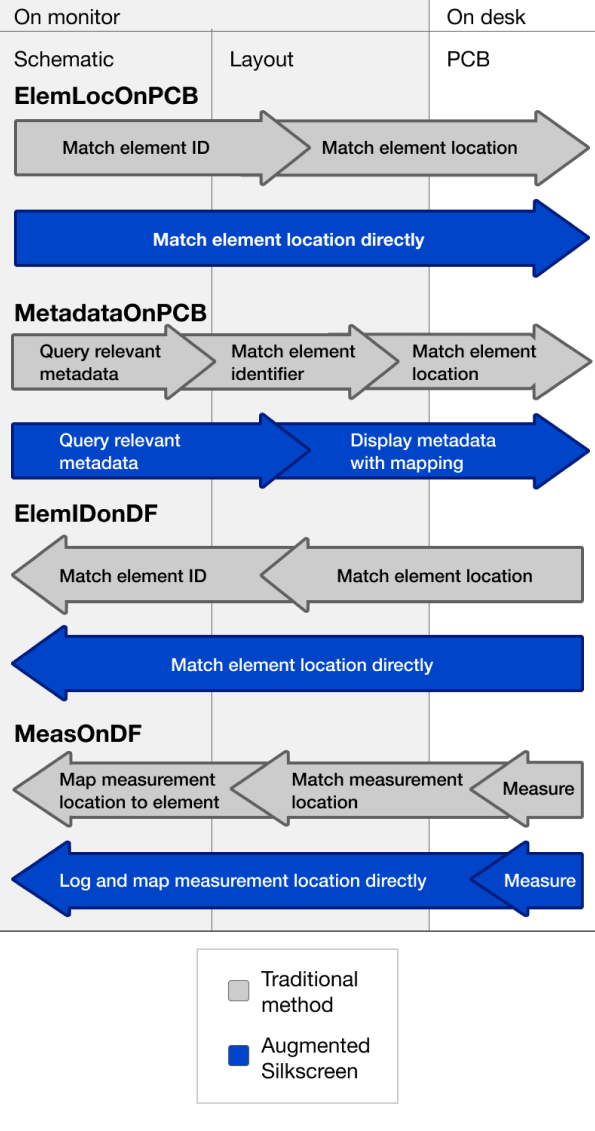
\includegraphics[width=.35\linewidth]{AS_figures/InformationFlow/Information-flow-scheme.jpg}
  \captionof{figure}{Information Flow of Core Interactions}
  \label{fig:InformationFlow}
\end{figure}
%\end{minipage}%
%\begin{minipage}{.5\textwidth}

\subsubsection{From Design Files to PCB}
The two core interactions relating design files to the PCB are \textit{element localization on PCB} and \textit{metadata annotation on PCB}.

\textbf{Element localization on PCB (\ElemLocOnPCB)}:
As per DC1, 
we found that engineers traditionally follow a two-step process to localize elements on the PCB given a target element on the schematic. First, they textually pattern-match an element identifier to the corresponding one in the layout file using the find command. Then, they spatially pattern-match the layout to the PCB to identify the corresponding PCB element.
%A few ECAD tools, such as Altium \cite{AltiumSoftware} and KiCAD \cite{KiCadSoftware}, support the notion of \textit{cross-probing}, where, if both the schematic and layout tools are open, an element selection in one will highlight the corresponding element in the other view.
A few ECAD tools \cite{AltiumSoftware, KiCadSoftware} support cross-probing between schematic and layout.
Using an AR system allows us to extend this interaction to the physical PCB, such that a selection in the layout or schematic view results in an augmented highlight of the matching design element directly on the PCB.

\textbf{Metadata annotation on PCB (\MetaDataOnPCB)}: During the process of debugging, engineers often query the schematic for element attributes that determine the function of the circuit, such as resistor values, IC packaging, diode reverse voltages, or inductor max currents. They keep this knowledge in short-term memory as they subsequently formulate hypotheses for a root cause or look to take their next diagnostic measurement.
As per DC1 and DC2,
we seek to minimize the cognitive load of keeping information in short-term memory by bringing this information to the PCB through annotating the PCB element with this element metadata in the view of the user.
Additionally, user-inputtable text field annotations can enable users to annotate elements with freeform notes.

\subsubsection{From PCB to Design Files}
The two core interactions relating PCB to the design files are \textit{element identification within design files} and \textit{measurement annotation within design files}.

\textbf{Element identification within design files (\ElemIdOnDesFiles)}: We learned that engineers follow the same two-step process as described in \ElemLocOnPCB~in reverse to identify or localize elements on the schematic given a target element on the PCB.
Pertinent to DC1, 
we propose enabling directly making selections on the PCB instead via an interactive probe to select, identify, and localize the same element within the schematic and layout. Probes are commonly used in PCB measurement tasks and are therefore a familiar method of direct PCB interaction.

\textbf{Measurement annotation within design files (\MeasOnDesFiles)}: Finally, taking diagnostic measurements is a key part of debugging workflows. \ASname\ would support this interaction by capturing measurement data from benchtop test equipment probed on the PCB and relaying it back to the design files addressing DC1 and DC3. As a practical implementation note, nearly all benchtop test equipment break out their \verb|get| and \verb|set| functions over SCPI/VISA, a standardized measurement instrument API.

\begin{figure}
  \centering
  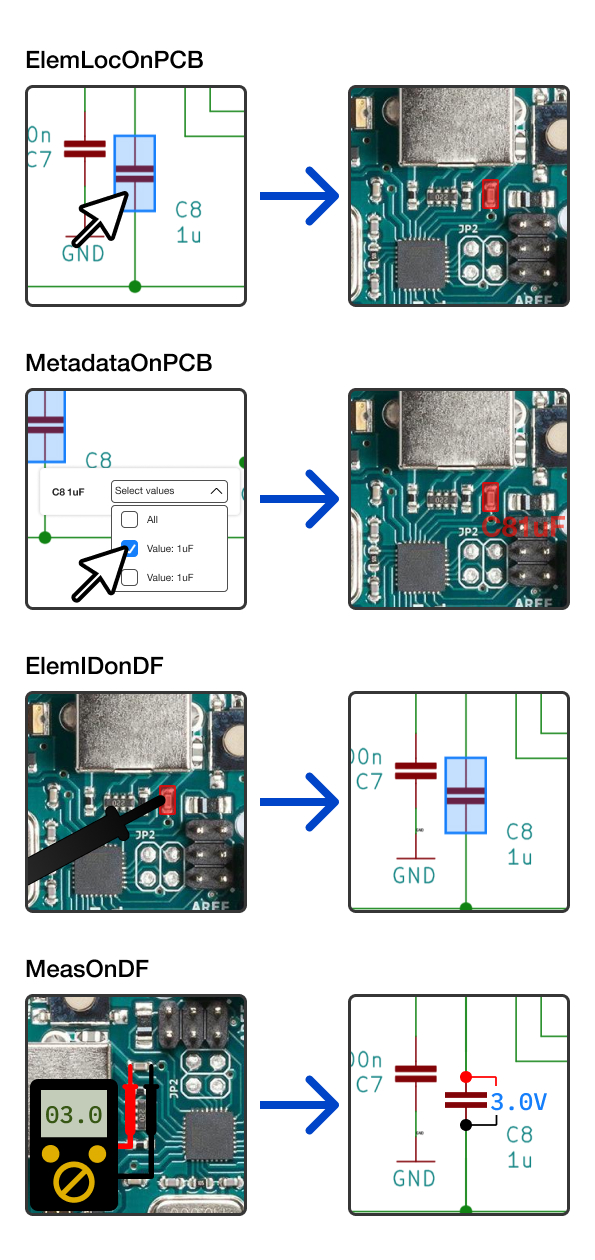
\includegraphics[width=.35\linewidth]{AS_figures/CoreInteractionDepictions/Core-interactions-depiction.jpg}
  \captionof{figure}{Depictions of \ASname\ core interactions}
  \label{fig:CoreInterationDepictions}
%\end{minipage}
\end{figure}

\subsection{Interaction Technique-Supported Workflows}
We synthesize these core interaction technique building blocks to support entire debugging workflows.

\subsubsection{Diagnostic Measurement}
Participants described the process of capturing and logging measurements as an important method to assist in deductive root cause analysis.
Combining the \ElemIdOnDesFiles\ and \MeasOnDesFiles\ interactions enables users to take a measurement with probes (\MeasOnDesFiles), capture the location the measurement was taken (\ElemIdOnDesFiles\ pin), identify the involved nets (\ElemIdOnDesFiles\ net), and include the information on the design file view along with the captured measurement.
%Combining the \ElemIdOnDesFiles\ interaction, specifically for purposes of pin identification and the \MeasOnDesFiles\ interaction enables users to take a measurement with probes, capture the location the measurement was taken, identify the involved nets, and include the information on the design file view along with the captured measurement.
For example, consider a user that wishes to record measurements, and so starts a new debugging session in \ASname's design file view.
The user may take a measurement of a voltage rail with a digital multimeter.
From the position of the probe locations on two pins, the corresponding nets for the positive and negative probe terminals are determined via \ElemIdOnDesFiles. The measurement value is captured along with its location in the design file view via \MeasOnDesFiles.

\subsubsection{Bring-up}
When engineers first apply power to their boards, they typically follow an exacting protocol to ensure all components were assembled properly.
By automating \ElemLocOnPCB\ interaction, all uninstalled component locations and all pin one locations (indicative of correct component orientation) can be highlighted directly on the PCB permitting rapid visual checks. Similarly, by entering a set of desired nets to test into the design file view, and optionally providing functional limits, \ASname\ can sequentially display probe points on the PCB, again via the \ElemLocOnPCB\ interaction. A user may then follow the \textit{diagnostic measurement} technique described above to sequentially capture the measurements back to the design files for comparison to set limits.

\subsubsection{Visual Inspection}
Participants described the need to sometimes query an element's metadata directly within the board view, for example, after noticing a given component's rise in temperature or in determining to which net a certain pin was connected. By combining \ElemIdOnDesFiles\ and \MetaDataOnPCB\, the user can select an element directly via probe on PCB and have the metadata annotated directly in the PCB view without having to refer to the design files.

\subsubsection{Remote Collaboration}
To facilitate remote collaboration, many participants pointed out the need to call out to specific elements on the board with a set of instructions.
In support of DC4,
this can be achieved by splitting \ASname's design file view and augmented PCB view across two locations.
Synchronous collaboration can be enabled if one user (for example, the board designer) has the design file view and the other user (the remote debugger) has the PCB.
The designer may select elements such as component or pins (probe locations) to display on the remote debugger's view of the PCB via \ElemLocOnPCB.
The \textit{diagnostic measurement} interaction may then be used to capture the remote debugger's measurement values back to the designer's design file view.
In an asynchronous collaboration, the designer could leverage the \MetaDataOnPCB\ interaction to tag elements in the PCB view with freeform instruction call outs. This could be helpful for communicating rework instructions or step-by-step debug procedures.

\section{Study 2: User Evaluation}
To solicit feedback on the interactions we designed, we remotely conducted another round of structured interviews using an interactive simulation. Each interview lasted approximately one and a quarter hours.

\subsection{Participants and Procedure}
For continuity, study 1 participants were re-invited to participate. Six out of the original eight participants were able to join (see Table 1). No additional participants were recruited. The study was divided into three main sections:

\begin{enumerate}
    \item Feedback on core interactions and interaction-supported workflows
    
    \item Feedback on variations on the attributes of core interactions 
    
    \item Timed element localization tasks  
\end{enumerate}

\subsubsection{Interview Assets}
To help participants envisage and solicit feedback on our interaction concepts during the remote interviews, we produced two artifacts: a web-based, interactive PCB simulator and a set of envisioning video sketches \cite{Vertelney1989UsingInterfaces}. The simulator mirrored the workbench setup described by participants in Sec. \ref{subsec:PrestudyFindings}. It comprised of two components: (1) an in-browser, interactive schematic and layout viewer on the participant's monitor (Fig. \ref{fig:Procedure-Part1}(A)) simulating the schematic and layout viewer an engineer would have open on their computer during debugging, and (2) an in-browser, interactive top-view PCB image on the participant's own touchscreen device (Fig. \ref{fig:Procedure-Part1}(C)) simulating the PCB the engineer would have on their lab bench during debugging. In order to deliver \ASname interactions that span design files and board augmentation, the two were linked via a web socket enabling real-time interaction in the schematic and layout viewer to affect augmentations on the mobile PCB view, and vice versa. Participants could select a component, pin, or net in either the schematic, layout, or mobile PCB view (via clicking or tapping via probe) and have the corresponding elements highlighted in the other two views. Additionally users could right click on a component revealing metadata and a button to show that metadata augmented on the PCB view (Fig. \ref{fig:Procedure-Part1}(A). Presenting interactions via this simulation prototype allowed for the users to use their own devices at home and allowed us to easily modify specific attributes of the way the core interactions were presented to users (see Sec. \ref{subsec:EvalAttributes}). This web socket could also be disabled to test situations without \ASname cross-linking between design files and board (see Sec. \ref{subsec:EvalSelectProcedure}). For the evaluation, we used the schematic, layout, and PCB image of an Arduino Uno R3\footnote{https://store.arduino.cc/usa/arduino-uno-rev3}.

Additionally, to further assist users in visualizing the interactions, we recorded a set of POV video walkthroughs for each interaction technique and each interaction-supported workflow. Each sketch illustrated the schematic and layout interactions in screen capture and view of a desk top PCB in a time-synced inset (ex. Fig. \ref{fig:Procedure-Part1}(D)). The PCB augmentations in the shown videos were projected via overhead projector (AAXA P7\footnote{https://www.aaxatech.com/products/p7-pico-projector.html}). A narration also helped to describe the interaction. During the interview, if the participant was unclear on the video content, the interviewer provided additional description until it was clear.

\begin{figure*}%[H]
    \centering
    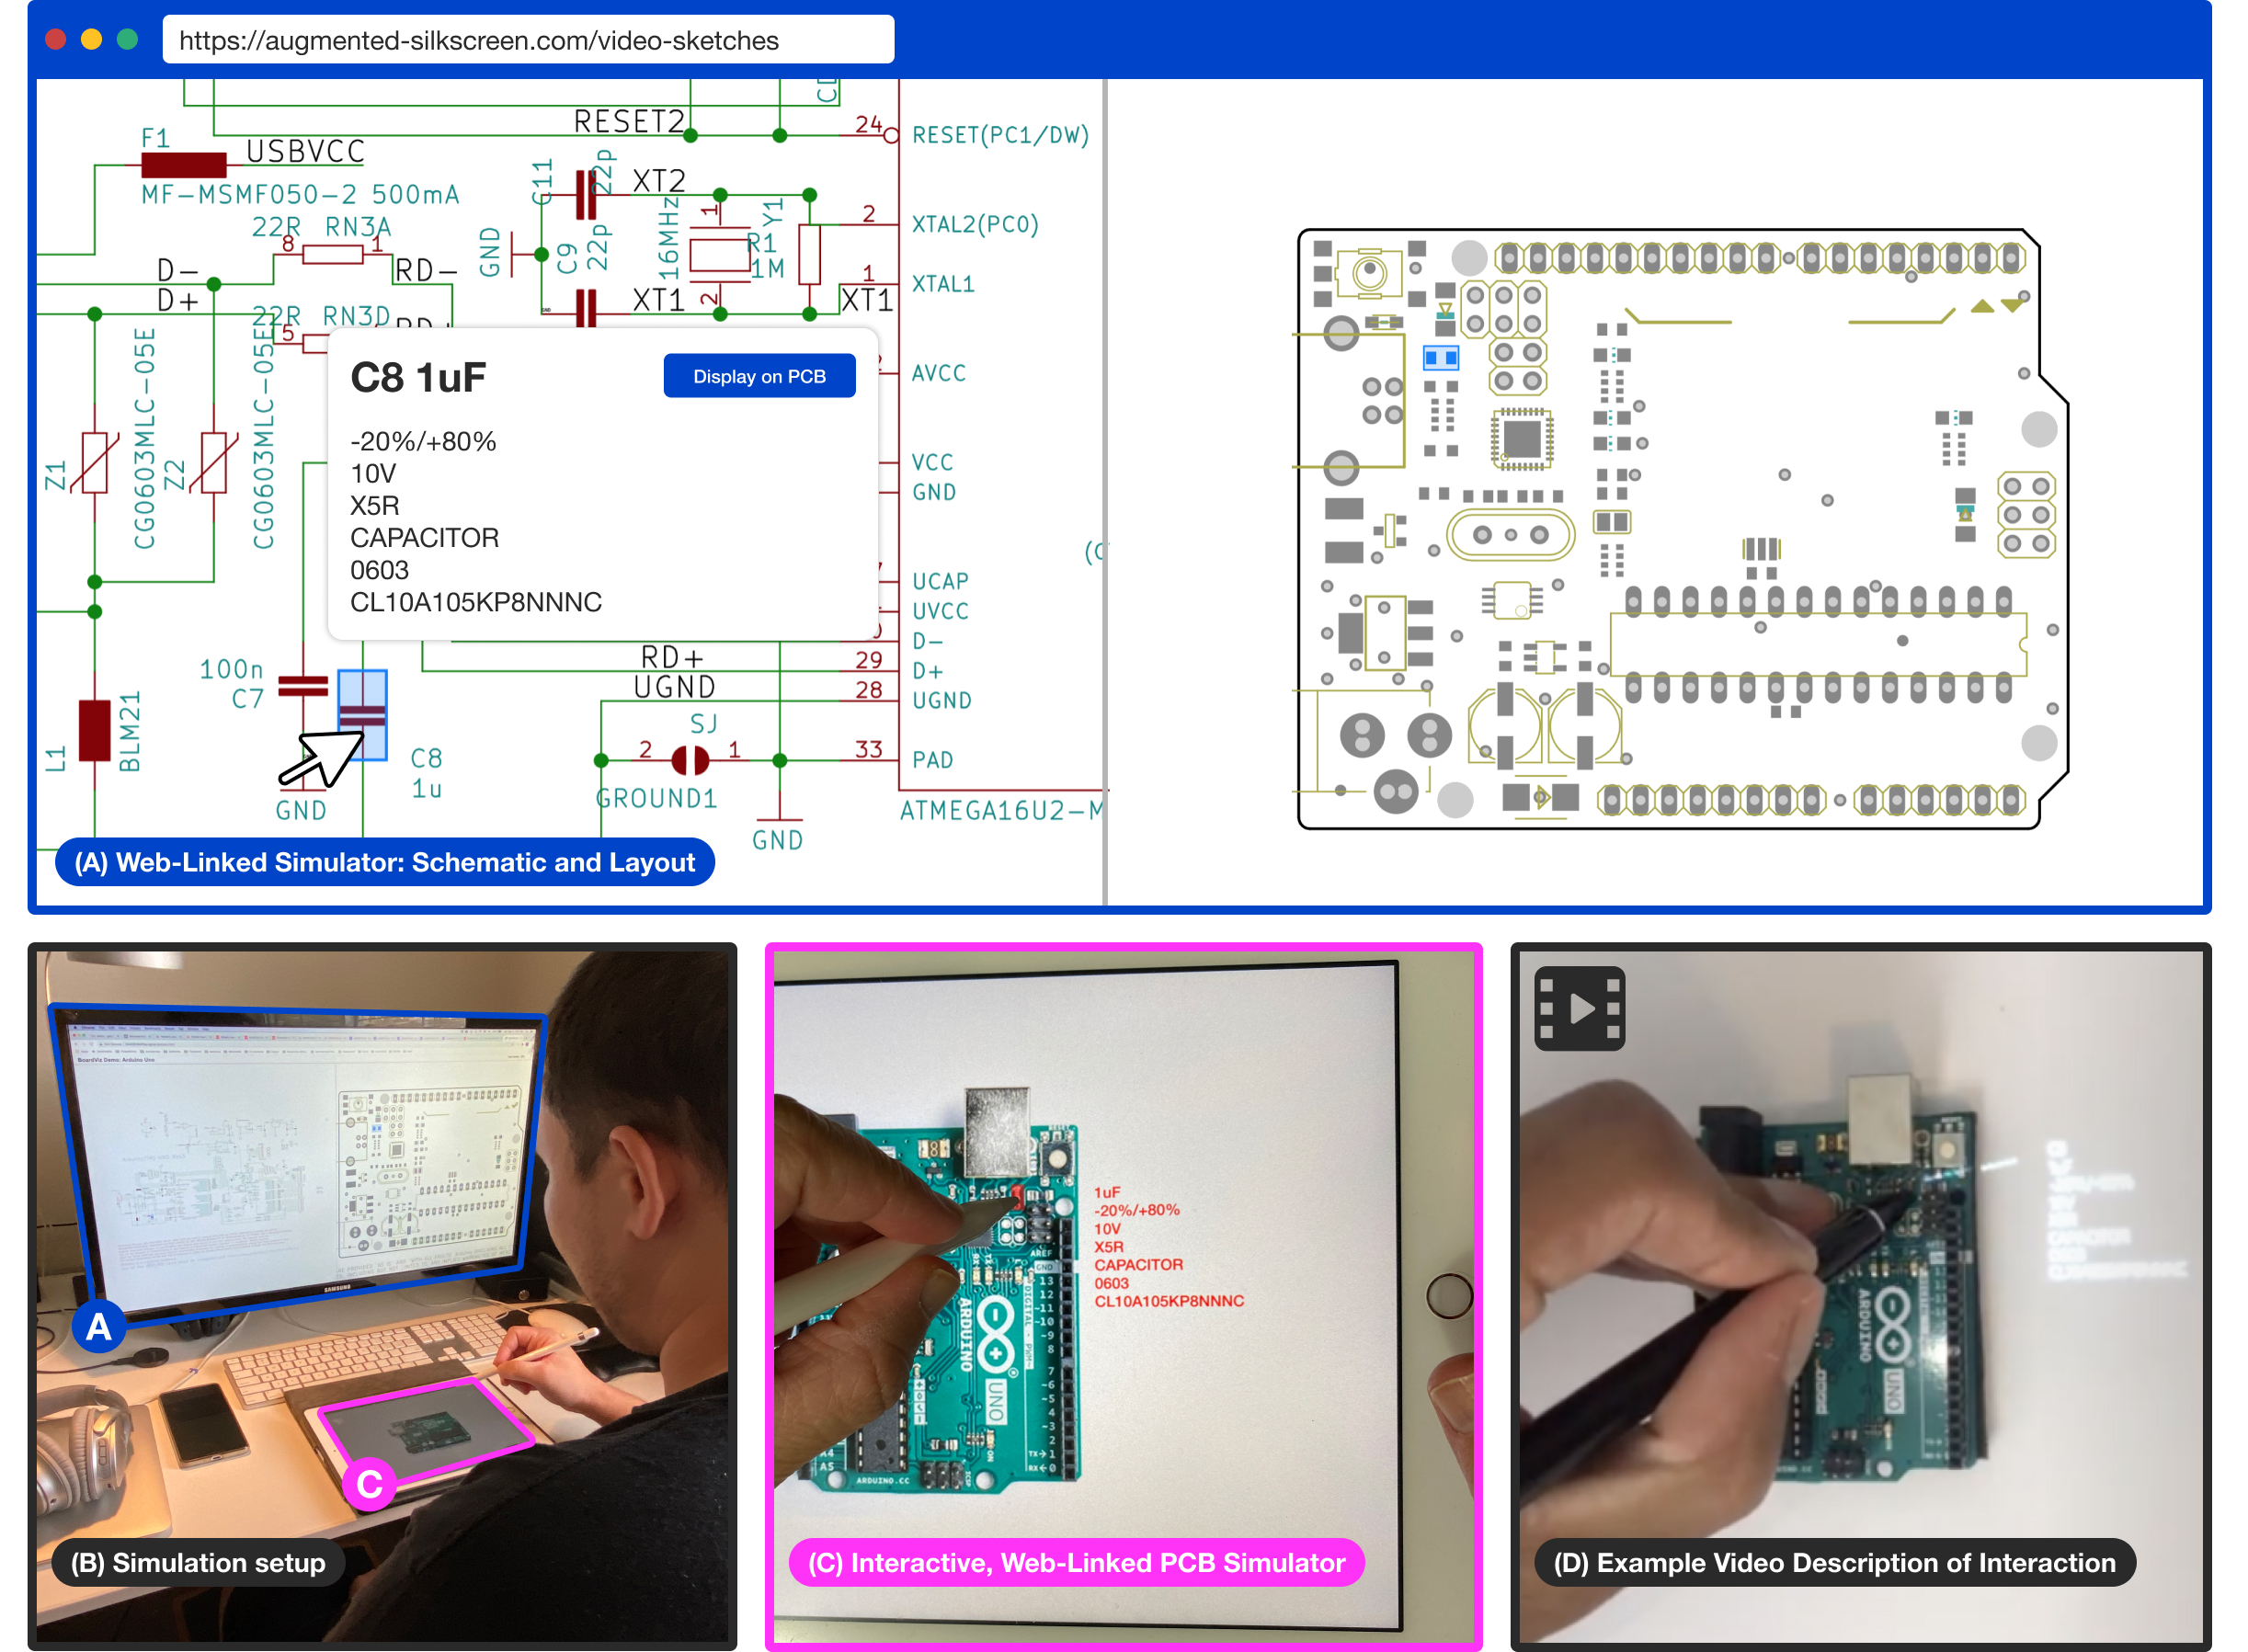
\includegraphics[width=0.9\linewidth]{AS_figures/Procedure-Part1/Figure-full-setup.jpg}
    \caption{The web-linked simulator consists of two components: an on-monitor design files viewer and an on-device PCB view. (A) In-browser canvases contain interactive views of the schematic (left) and layout (right) of the design, just as engineers would have on their monitor during PCB debugging. Here, the user has selected capacitor C8 in the schematic (A, left), which would cause the corresponding element to highlight in both the layout (A, right) and PCB view (C). (B) A remote participant has the simulator open on their monitor and touch screen device. (C) The PCB simulator imitates a PCB a user would have on their desk. Here, a component is augmented with a box highlight and a metadata annotation. A user can use a probe to interact with the PCB simulation, which would affect the state of schematic and layout (A). (D) Freeze frame of inset from an example video description (Visual Inspection video). The video actually shown to the user contains a time-synced screen recording of design file view (A) with (D) inset picture-in-picture.}
    \label{fig:Procedure-Part1}
   
\end{figure*}

% \subsubsection{Interactive Prototype}
% For the interactions testing, we've built an interactive prototype which consisted of two main parts:
% \begin{enumerate}
%     \item Desktop web-page that imitated layout and schematic debugging setup on the monitor
%     \item Mobile web-page that imitated a physical PCB of Arduino Uno
% \end{enumerate}
% In addition to the web-prototypes, each of the participants were sent out a stylus that imitated a physical probe for interaction with the virtual PCB.

\subsubsection{Part 1 Procedure}
% Participants were shown 11 different videos sketches [ref needed] depicting the interactions and supported workflows. Each sketch illustrated the schematic and layout in screen capture and view of the PCB in a time-synced inset (Fig. \ref{fig:Procedure-Part1}). The PCB augmentations in the shown videos were projected via overhead projector (AAXA P7\footnote{https://www.aaxatech.com/products/p7-pico-projector.html}). The video both visually demonstrated the actions. The actions were also narrated by voice.
% If the participant was unclear on the video content, additional description was provided until it was clear.
The participant was shown each video sketch and the interactive simulator, starting with core interaction techniques and ending with interaction-technique supported workflows. Between each video sketch, the participant was then verbally asked the following questions:
\begin{enumerate}
    \item \textit{``Would you find this interaction to be helpful, not helpful, or have no impact on your debugging workflow?''}
    \item \textit{``How might this interaction affect your workflow?''}
    \item \textit{``How likely would you be to adopt this interaction on a scale from 1 (would not use) to 7 (very likely to adopt)?''}
\end{enumerate}
We analyzed responses via thematic analysis \cite{Braun2006UsingPsychology}, by transcribing the interviews, coding recurring themes, and noting outliers.

\subsubsection{Part 2 Procedure}
To better understand how certain design decisions align with the stated design guidelines, we asked participants to assess variations on attributes of the core interactions in five categories
(Fig.
\ref{fig:Procedure-Part2}):

\begin{figure*}
\centering
    \centering
    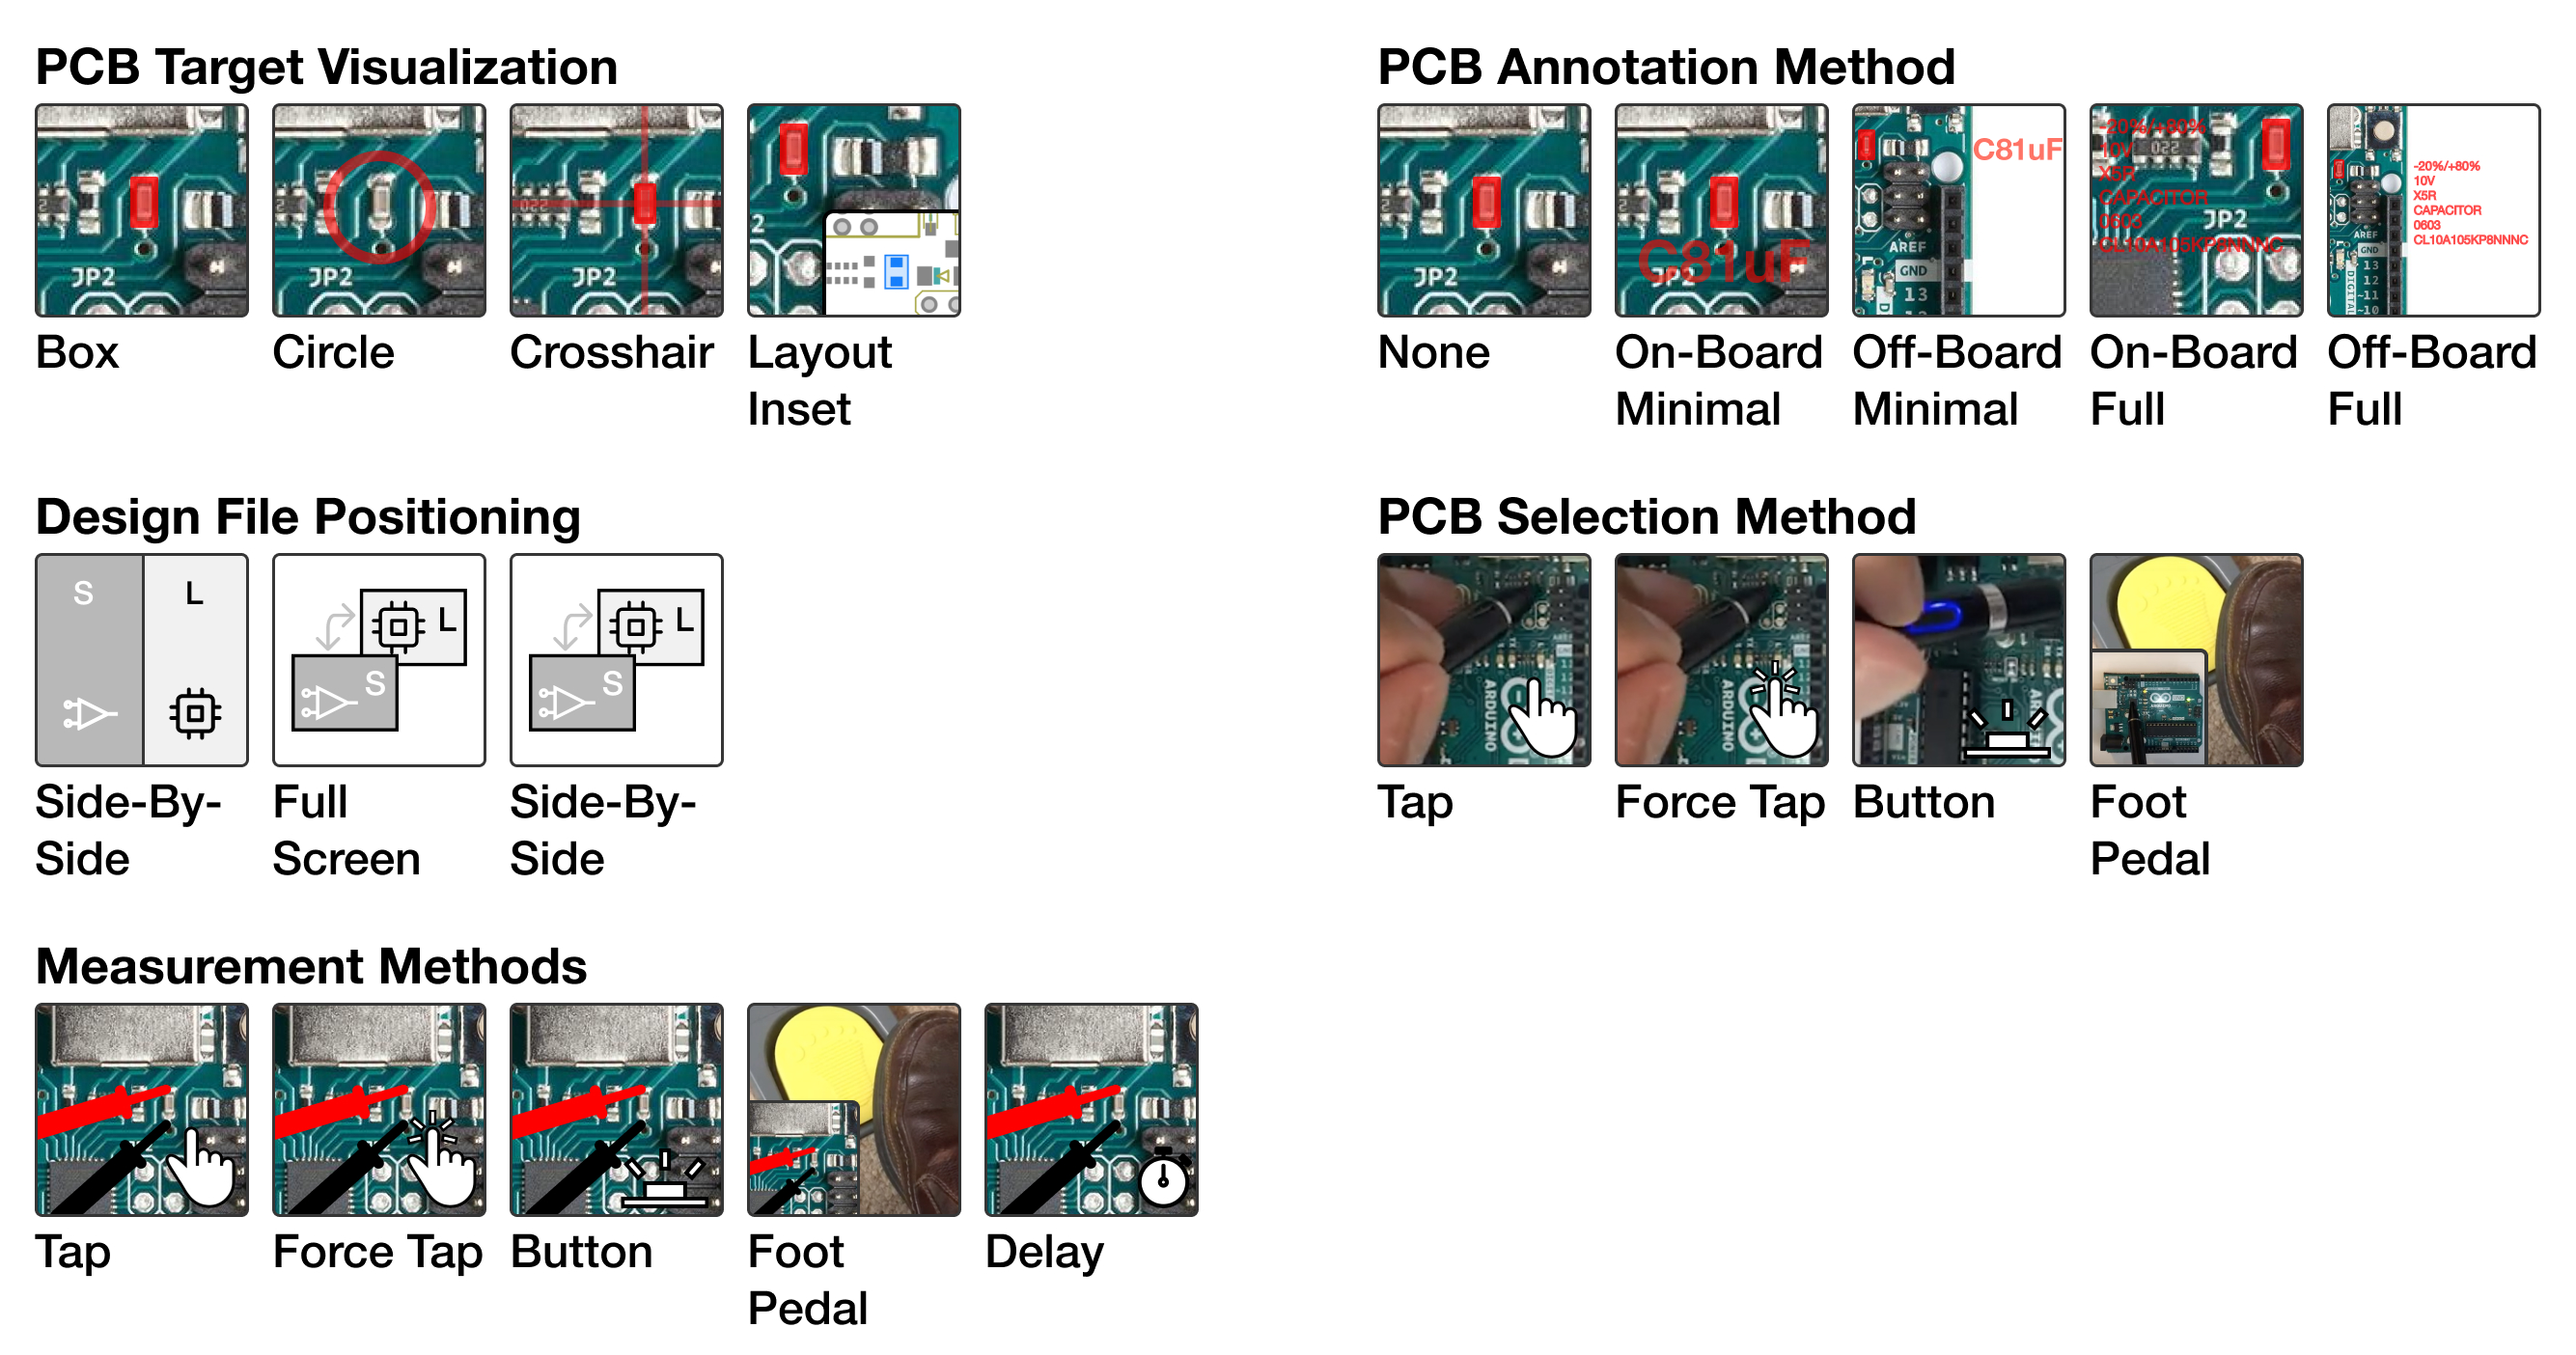
\includegraphics[width=0.7\linewidth]{AS_figures/Procedure-Part2/Attributes.jpg}
    \captionof{figure}{The matrix of variations we presented to participants to elicit design feedback on attributes of the core interactions.}
\label{fig:Procedure-Part2}
\end{figure*}

\begin{enumerate}
    \item \textit{PCB Target Visualization:} Per DC2, how does the visual design of augmentation influence element localization in \ElemLocOnPCB? Options: (a) Box---filled in rectangle, (b) Circle---unfilled circle, (c) Crosshair---perpendicular, intersecting lines, (d) Layout inset---highlight is shown briefly, an inset segment of the layout local to the target element is projected next to the board
    \item \textit{PCB Annotation Method:} Per DC2, what is the preferred length and where is the preferred area for on-board annotations in \MetaDataOnPCB? Options: (a) None---no annotation, (b) On-board minimal---annotation depicting only element identifier and value projected adjacent to the element (potentially overlapping the PCB), (c) Off-board minimal---only element identifier and value; projected on tabletop adjacent to the board, (d) On-board full---all element metadata fields projected adjacent to element, (e) Off-board full---all element metadata fields projected on tabletop
    \item \textit{Design File Positioning:} Per DC1, how the positioning of design files on monitor influence element identification within design files in \ElemIdOnDesFiles? Options: (a) Side-by-side, (b) Full screen---schematic and layout each took entire screen, flipped between files, (c) Layout inset---layout local to the target element is inset on schematic view
    \item \textit{PCB Selection Method:} Per DC3, what is the preferred method to trigger selection of PCB elements with a probe for \ElemIdOnDesFiles? Options: (a) Tap---tap top of element briefly to select, (b) Force tap---similar to BoardLab, applying force to probe tip triggers selection, (c) Button---button on barrel of probe triggers selection, (d) Foot pedal.
    \item \textit{PCB Measurement Capture Method:} Per DC3, what is the preferred method to trigger a measurement capture on PCB with a probe for \MeasOnDesFiles? Options: (a) Tap---tap pins to capture selections, (b) Force tap---applying force to probe tips triggers capture, (c) Button---button on barrel of probes triggers capture, (d) Foot pedal, (e) Delay---stationary probes for 3 seconds triggers capture.
\end{enumerate}

% \begin{figure}
% \centering
% \begin{minipage}{.5\textwidth}
%     \centering
%     \includegraphics[width=.9\linewidth]{AS_figures/Procedure-Part4/Procedure-Part4 v2.jpg}
%     \captionof{figure}{Participants performed the timed element localization task remotely on a PCB stand-in. (A) monitor with schematic and layout views, (B) touch screen device as interactive PCB stand-in, (C) capacitive stylus as probe stand-in.}
%     \label{fig:Procedure-Part3}
% \end{minipage}%
% \begin{minipage}{.5\textwidth}
%     \centering
%     \includegraphics[width=.9\linewidth]{AS_figures/Procedure-Part2/Attributes v6.png}
%     \captionof{figure}{The matrix of variations we presented to participants to elicit design feedback on attributes of the core interactions.}
% \label{fig:Procedure-Part2}
% \end{minipage}
% \end{figure}

Items (1), (2), and (3) were delivered via the interactive web simulator.
%Users used their own monitor and touchscreen device with a PCB image as stand-in for a real board, where simulated augmentations could be delivered.
Items (4) and (5) were described with the video sketches. After the demonstration, we asked participants about their general impressions, how they would rank the presented variations, during which workflow they might use it, and why.

\subsubsection{Part 3 Procedure}
\label{subsec:EvalSelectProcedure}
Users performed two timed component selection tasks: finding components on the board given a target in the design files, and finding a component in the schematic given a target on the board. An interactive web simulator delivered the schematic and layout on their monitor, and a PCB image stand-in on their touchscreen device in an imitation workbench set up (Fig. \ref{fig:Procedure-Part1}(B)).
A standard capacitive stylus shipped to the participants was used to select components on the PCB. For the \textit{find on PCB task}, a target component was highlighted on the schematic and layout.
The user’s task was to select the corresponding component on the board. When \ASname\ (cross-linking between design files and board) was enabled, the target component on the board had an augmented highlight as well.
For the \textit{find on schematic} task, a target component was highlighted on the board.
The user’s task was to select the corresponding component on the schematic. Selection cross-linking between the layout and schematic as in KiCAD~\cite{KiCadSoftware} was enabled as baseline. When \ASname\ was enabled, the target component on the schematic and layout were highlighted.
For each task, all six users performed twenty different component selections: ten selections with \ASname\ and ten without, with order randomized (for a total of 60 samples per condition minus omissions).
%The order components were presented to the users were randomized.
Users were permitted a short practice round to familiarize themselves with the selection task.
Audio feedback indicated if a user selection was correct or not.
Schematic and layout visualizations were kept the same between conditions.
Timing started when the component to be found was presented to user (on the schematic and layout in the \textit{find on PCB task} and on the board in the \textit{find on schematic task}). Timing stopped when the user selected the correct corresponding component (on the board in the \textit{find on PCB task} and on the schematic in the \textit{find on schematic task}).
If a user selected the incorrect component, the data was logged as a mistarget; if a user indicated it was due to a fault of the capacitive stylus or touchscreen, rather than a true mistarget, the datum was omitted.

\subsubsection{Findings from Part 1: Feedback on Core Interactions and Interaction Supported Workflows}
\label{subsec:EvalCoreInteractions}

\begin{figure*}
    \centering
    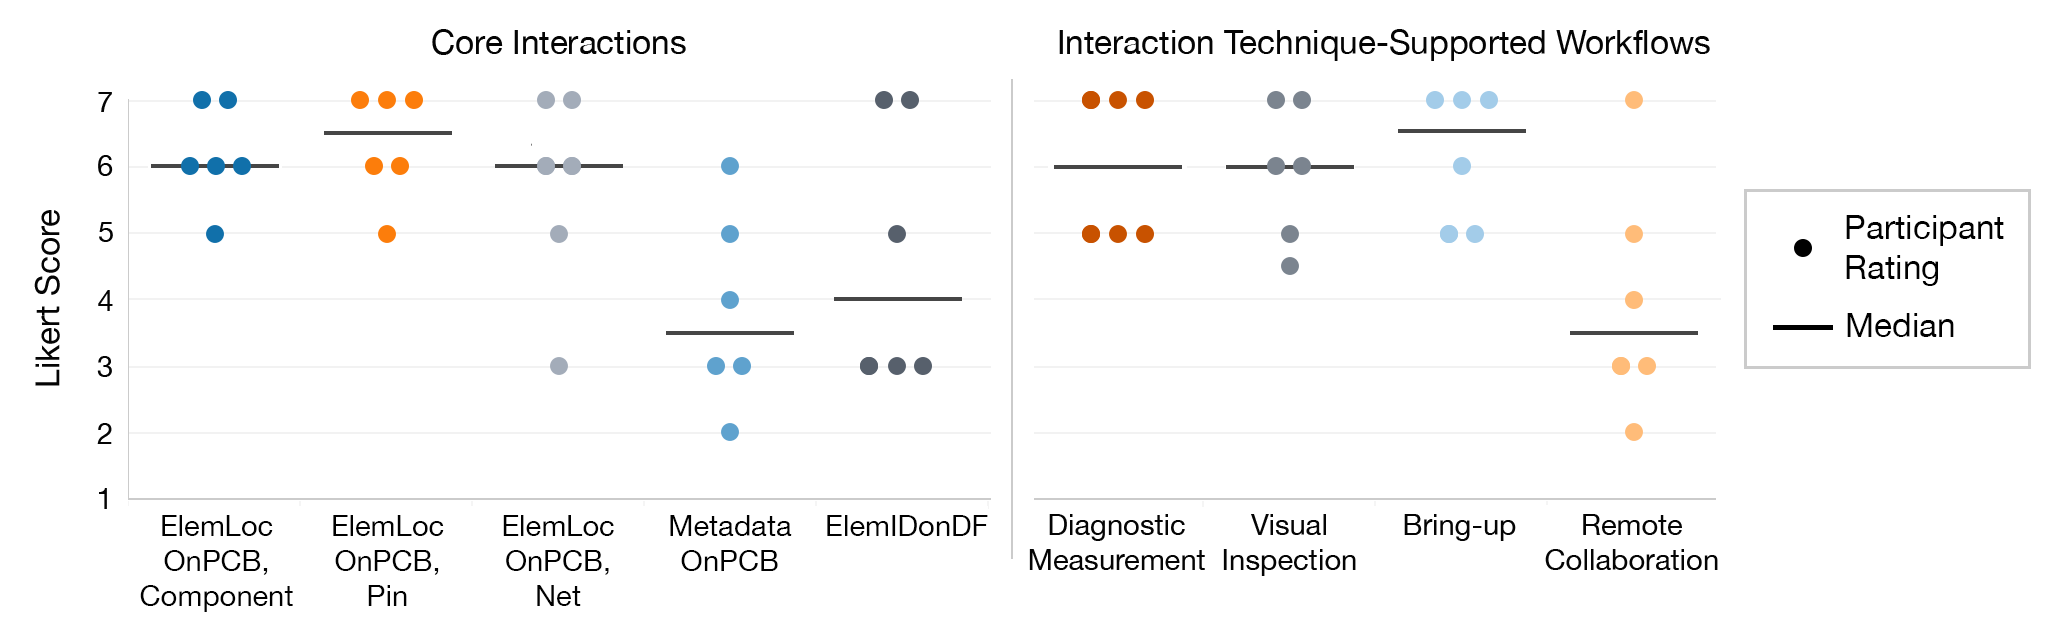
\includegraphics[width=0.85\linewidth]{AS_figures/Graph-Part1/graph-part1and3-v5.png}
    \caption{Results from Part 1 (core interaction and workflow feedback).}
    \label{fig:Eval-Part1}
\end{figure*}

Users provided illuminating feedback on their preferences and uses of the core interactions and workflows (Fig.~\ref{fig:Eval-Part1}).

Users unanimously rated EL-PCB favorably for localizing components, pins, and nets.
% Every participant agreed that when finding components:
\textit{``It basically saves me an extra step\ldots this allows me to go from schematic to board immediately''} (P1,~\sharcHere{q:saves_step}).
\textit{``I have to do it pretty much manually in different pieces of software. So, this would have saved me a lot of time''} (P6,~\sharcHere{q:different_software}).
% \textit{``There’s no reason I would look at the board file if I had this feature''} (P7).
Specific situations in which EL-PCB would be particularly helpful included working with complicated and dense boards (P1), unfamiliar boards (P2), or boards without silkscreen (P5).
P7 also pointed out that \textit{``trying to find specific patterns, especially with things are rotated and whatnot is very error prone''} (\sharcHere{q:patterns-rotated}) for humans, and that computationally-driven augmentation can help to disambiguate.
%it is computationally much simpler and this technique could simplify that.


% Users called out specific situations where this would be helpful:
% \textit{``especially for complicated boards with a lot of different capacitors or resistors''} (P1). 
% \textit{``Super helpful\ldots especially navigating either a new board that I'm not super familiar with or a design I haven't touched in a while''} (P2). 
% \textit{``when the reference designator isn't on the silkscreen. Then it's like, you know, you have to like dive into the Gerber files, and then like hover over the part to get the reference designator''} (P5).

% For pins, much the same feedback was shared across the board\footnote{no pun intended}: % NUUUUU losing the pun :( %NUUUUUUUUUUU
% \textit{``it’d save me the step of referencing the datasheet''} (P1).
% \textit{``I feel like would actually be even more useful than just finding the component, and a lot of scenarios because I'm trying to find specific patterns, especially with things are rotated and whatnot is very error prone''} (P7).

P1 cited that there might be practical issues with the precision of an AR system highlighting very small details (the 500~{\textmu}m
pitch pins of a QFN24 package), and P5 raised concerns with the potential for trust issues if the projections were inaccurate: \textit{``this would be useful but misleading, because yeah what if they got stuck with the wrong part.''} (\sharcHere{q:misleading})
% \textit{``I can see that, for example, like the QFN24 [(an IC package with 500um pitch pins)], the pins might be way too close together to highlight a single pin''} (P1), but another pointed out
As P7 pointed out, however, \textit{``as the pitch gets more and more fine, being able to identify the pin doesn't help quite so much, because there's not a lot you can do if it's so small that you can't probe it [anyway].''} (\sharcHere{q:not_a_lot})

Nonetheless, highlighting specific pins connected to a given net was also liked, specifically to identify suitable measurement probe points for a given net:
% \textit{``It's very helpful, especially when, like in industry boards you don't have super easy access points with all of your components so sometimes some of these nodes would fall under like an EMI shield [(metal covering over components to reduce electromagnetic interference)]''} (P2).
\textit{``[when] looking for a component that was easy to probe without shorting anything else nearby\ldots I don't even have to worry about like looking through the package size on the schematic sheet and trying to find something that's like on the net that's going over different schematic pages. [With augmentation] I can just literally look at the board and say, `Oh, I got this big capacitor right here that has a good probing point.'''} (P6,~\sharcHere{q:big_capacitor}).
Another user looked to use this feature to locate accessible nodes since many are obstructed by features such as shield cans or mechanical cases ``in industry boards.'' (P2,~\sharcHere{q:industry_boards}).
% \textit{``I even today did something pretty similar\ldots I was looking for a component that was easy to probe without shorting anything else nearby\ldots Then I don't even have to worry about like looking through the package size on the schematic sheet and trying to find something that's like that on the net that's going over different schematic pages. I can just literally look at the board and say, `Oh, I got this big capacitor right here is that has a good probing point.'''} (P6).

% One user (P1) interpreted localizing a net as highlighting a (potentially buried) trace, rather than connected pins, mentioning this would be applicable only in rare situations where they would need to uncover or sever a trace with a knife, and, therefore, said they were unlikely to use it often.

As an interaction in and of itself, \MetaDataOnPCB\ rated poorly, with many users citing that selecting metadata on the schematic to display within the board view was redundant: 
\textit{``If I'm already on the schematic and the information is there on the schematic it's not super helpful to display it again on the side of the board.''} (P2,~\sharcHere{q:redundant}).
% \textit{``I would say if information if I'm already on the schematic and the information is there on the schematic it's not super helpful to display it again on the side of the board.''} (P2).
However, when combined with EI-DF to form the Visual Inspection interaction (allowing users to trigger augmented metadata annotations directly from the board as opposed to the schematic) the interaction was universally preferable. 
% \textit{``You touch it on the physical board and then it gives you information, that I could totally see being helpful. Because a lot of the time it's [referring to the metadata] not there [on the PCB].''} (P8).
\textit{``I'm doing this 24/7, like which pin is which\ldots if I could do something to where I could just be looking at the board, and not have to look away, and just having it projecting on top of it. That would be -- oh my god -- I would use that like 100\% of the time.''} (P5,~\sharcHere{q:oh_my_god}).
P2 added that \textit{``in factory environments\ldots this feature could limit the number of different screens or devices I need to carry around.''} (\sharcHere{q:carry_less})
% P2 indicated that \textit{``in factory environments\ldots this feature could limit the number of different screens or devices I need to carry around... so if I can just have the circuit board in front of me and get that info.''}

% Many users also expressed the Visual Inspection interaction as useful to assist in assembling boards.
% Like MA-PCB, EI-DF received mixed reviews for functionality as a stand alone interaction.
% \textit{``I think it can be helpful but less so than the other way around [EL-PCB]\ldots Normally I feel like you would know what [component] it is, if it's your design, so it'd probably be more helpful on a design you're not familiar with''} (P6).
% It only became universally useful when combined with other interactions.

Diagnostic Measurement workflow was found to be helpful in not only alleviating an individual's own mental demands but also in capturing unambiguous logs for documentation and interacting with others.
% capturing the measurement location and logging the values themselves.
% \textit{``As far as like actually debugging goes\ldots I definitely see it being a useful feature in terms of like recording the actual results\ldots I've had personally a whole lot of negative experiences of people measuring the wrong things and telling us that they got such and such results.''} (P8).
% \textit{``In a case where like, Oh, I have this dead board, I don't know what what exactly is wrong with it. I can open up like a debug session you could call it. And instead of me pre-defining what rails I want to measure, if I could just go and measure rails and it could tell that like I'm measuring VSYS [system voltage rail], or 3.3[V rail], and it's just logging like a new line item every time then that would be super useful''} (P6).
\textit{``This would be extremely helpful, because... what I've been doing up until this point is, I may like probe something and then I'll just keep in the back of my mind like okay it's this value. And then I'll just keep like three to four values in my head''} (P5,~\sharcHere{q:back_of_my_mind}).
% \textit{``this is, yeah this is great, This would be extremely helpful, because... what I've been doing up until this point is, I may like probe something and then I'll just keep in the back of my mind like okay it's this value. And then I'll just keep like three to four values in my head''} (P5).
\textit{``I've had personally a whole lot of negative experiences of people measuring the wrong things and telling us that they got such and such results.''} (P8,~\sharcHere{q:wrong_things}).

% One user appreciated the fact that the measurement value could be projected as well next to the board: 
% \textit{``trying to look at multimeter while you're probing small components is difficult, so just being able to see it next to your board will be helpful.''} (P7).

All participants appreciated the interaction technique-supported Bring-Up workflow:
\textit{``very helpful useful during board bring-up, we're just trying to take a basic DC measurement on multiple nodes quickly, smoke test\ldots a lot of times that's tens of nets that we're trying to measure,\ldots and if we can very quickly step through that without having to go back and forth between the board and the PC recording and Excel or whatever, would definitely save a lot of time.''} (P2,~\sharcHere{q: bring_up_basic_measurement}).
\textit{``I could see this like cutting down board bring-up down in time by like hours.''} (P5,~\sharcHere{q:by_like_hours})
%\textit{``This would be a huge game-changer for validation and board bring-up. I could see this like cutting down board bring-up down in time by like hours.''} (P5)
% \textit{``super useful for board bringup or for validation testing, because if you have to develop test plans anyways, test cases. So if part of that was like I just put the test case in this format and it just has a list of rails that I need to measure and it just highlights, `oh yeah, measure this rail' and it highlights where I need to measure on the board and it's just automatically populating everything for me, like, that would be great.''} (P6).
Some users suggested they also found it useful to define and project probe points for unstructured debugging: 
\textit{``[I'm] interested in just the fact that it can highlight the two things I want to probe at the same time though so I know exactly where to put those probes.''} (P1,~\sharcHere{q:exactly_put_probes}).
The explicit probe point projections inspired some users to suggest it can assist train those unfamiliar with their design.
\textit{``If I was giving this to like a, like undergrad or like an intern or something you know, probably be pretty useful for them just to quickly catch on''} (P1,~\sharcHere{q:undergrad}).
% \textit{``if I wanted to test like many boards like if I was doing like a, like a long run up like 10 to like 50 boards or or especially if I was giving this to like a, like undergrad or like an intern or something you know, probably be pretty useful for them just to quickly catch on''} (P1).
\textit{``If you\ldots can turn this [probe point projection] into an automation program\ldots this would be great at a factory.''} (P5,~\sharcHere{q:automation}).
% \textit{``If you get like 100 boards in maybe you just you want to do a quick quick run, you know? Then you can turn this into an automation program too\ldots when it comes to factory workers, you know, this would be great at a factory.''} (P5).

Finally, the Remote Collaboration scenario received a varied set of rankings. One user, affected by remote work during the recent COVID-19 pandemic said,
\textit{``I think just the ability to communicate very unambiguously; not only like what part, you know, because you could use the reference designators in like an email or a phone call or whatever to tell people what to look at, but, like, in terms of selecting actual points to measure. I think that would be super helpful. Personally, what I've had to do a lot of recently is taking pictures of the manufacturing preview, and then like drawing a circle on what we need and then sending that back and forth on Slack. And so just, you know, in the sense that, that will speed that up a lot.''} (P8,~\sharcHere{q:unambiguously}).
% \textit{``I think the idea would help organize the process.''} (P5).
Many users thought the interactions were useful, but were not frequently involved in collaborative debugging situations. They recognized that they may have growing utility as the pandemic continues to affect workplaces:
\textit{``I think [these interactions] can be useful and especially I guess in a situation like we have right now where everyone's work-from-home. And if I don't want to go to a factory, and there's lab techs at the factory, and they're there trying to figure out what's wrong with the board, and they don't necessarily have the expertise about that board, I could probably walk them through it and highlight stuff\ldots I could see it useful in that kind of situation but it's more of a hypothetical because it's not something that I've really done much yet myself.''} (P6,~\sharcHere{q:hypothetical}).
% \textit{``I haven't really had a project where I feel like remote debugging was super needed. Like oftentimes, obviously, most of the time debugging, happens in-person, even if you're having someone else help you do it. Obviously with like current scenario like I can definitely see why this could be interesting.''} (P1).
One user also expressed that it’d be helpful to point out to their software colleagues certain buttons, switches, and plugs to interact with on their development kit, but they are not often in situations where the other user would be actively probing pads.


\subsubsection{Findings from Part 2: Feedback on Core Interaction Attributes}
\label{subsec:EvalAttributes}

\begin{figure}
\centering
%\begin{minipage}{.5\textwidth}
  \centering
  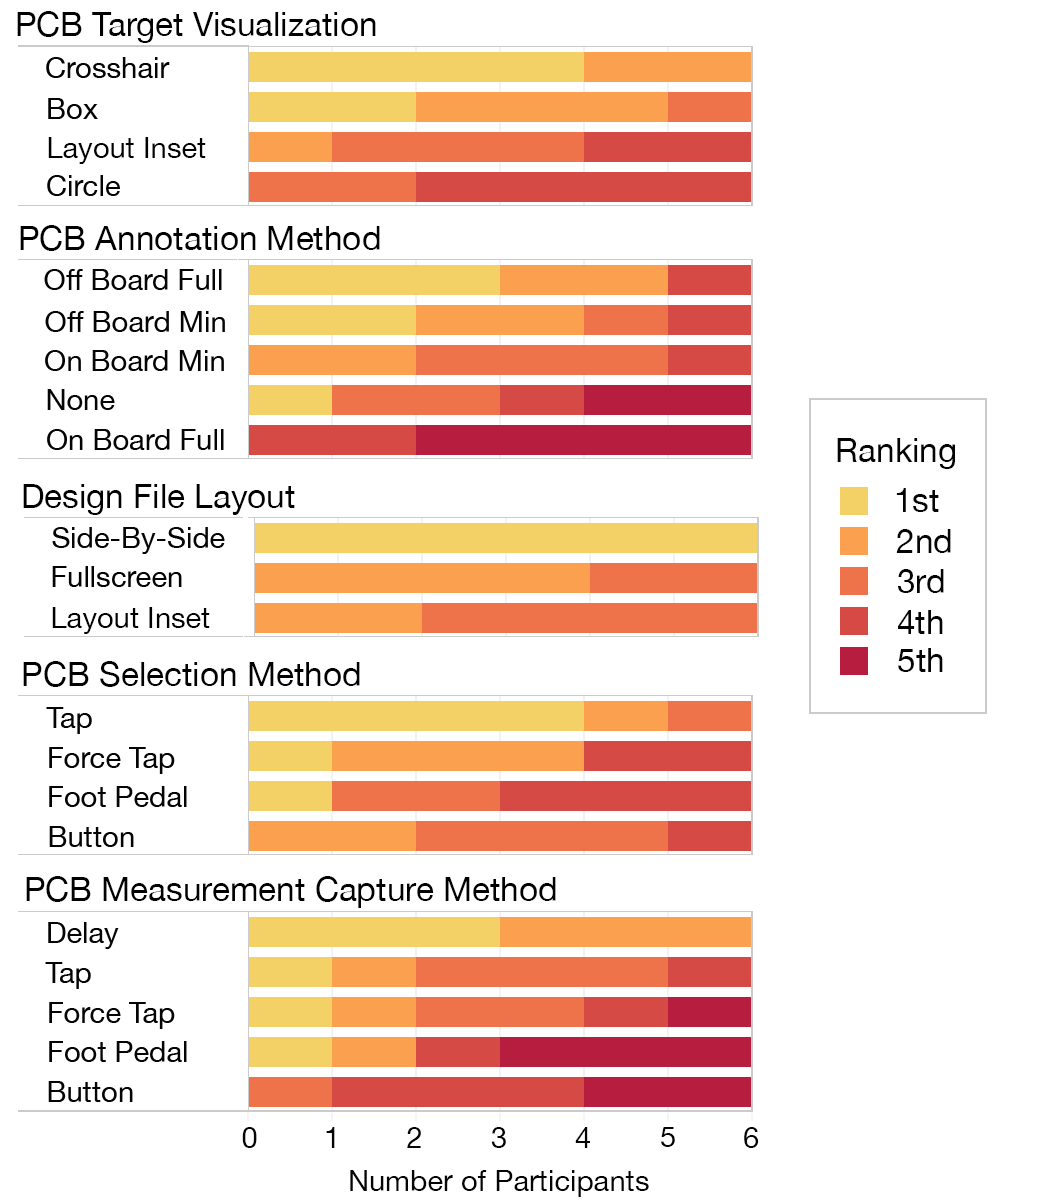
\includegraphics[width=.9\linewidth]{AS_figures/Graph-Part2/graph-part2-v3.png}
  \captionof{figure}{Results from Part 2 where users ranked their preferred variations of core interaction attributes.}
  \label{fig:Eval-Part2}
%\end{minipage}%
\end{figure}
\begin{figure*}
%\begin{minipage}{.5\textwidth}
  \centering
  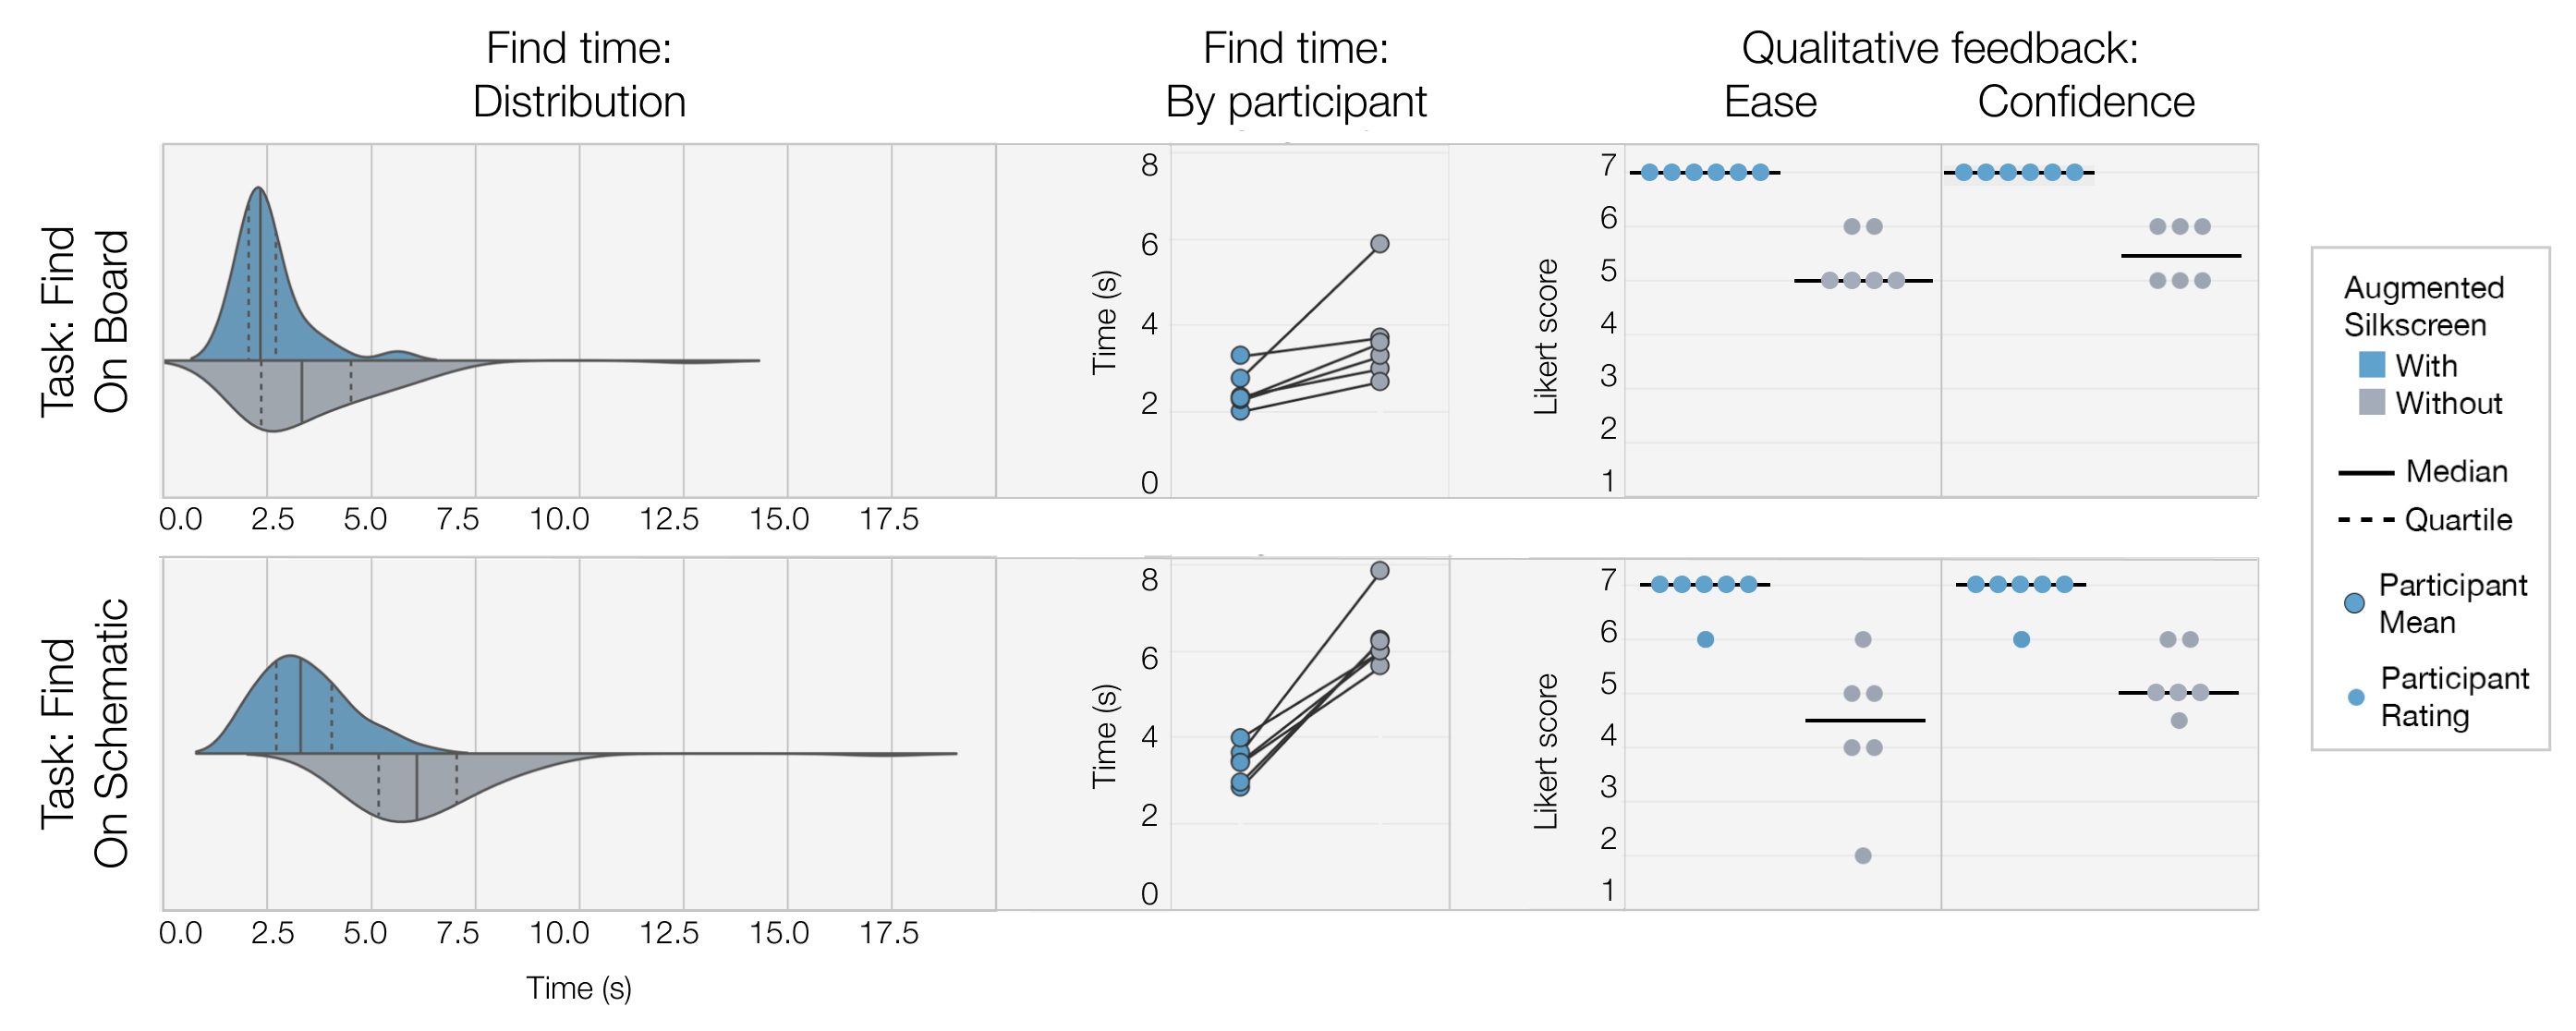
\includegraphics[width=1\linewidth]{AS_figures/Graph-Part4/Graph-part4-v4.jpg}
  \captionof{figure}{Results from Part 3 where users participated in a timed element localization task.}
  \label{fig:Eval-Part3}
%\end{minipage}
\end{figure*}

Users ranked target visualizations for \ElemLocOnPCB. Crosshair was the primary choice, but box was seen as nearly as good.
\textit{``The crosshair makes it super easy to individually pick out which one is which''} (P7,~\sharcHere{q:crosshair_easy}). \textit{``box one is my favorite because it superimposes the most accurately on the part of interest''} (P5,~\sharcHere{q:box_favorite}).
A user suggested that a crosshair transitioning to a box is good for initial targeting and reducing visual clutter.
The circumscribed circle was missing the details of the component's contour, reducing visual precision and as a result being ranked lowest among most participants. 
\textit{``The circle is misleading because it's like encompassing multiple parts''} (P5,~\sharcHere{q:circle_misleading}).
Towards this end, an AR system must be precise enough to provide unambiguous augmentations on PCB elements (which can be less than millimeter square for the smallest pins).
To help resolve ambiguous cases, a local inset of the layout was appreciated as visual confirmation, but users looked for it to be combined with an on-board visualization rather than as a standalone method.

Toward annotating metadata on the board (\MetaDataOnPCB), participants generally preferred off-board annotations (indicating that on-board annotations felt cluttered), but there was disagreement on how much information to present---between our options presented, there was an even split between all metadata or none, suggesting there is likely some ideal middle ground.
Some users indicated their preference would be to control what metadata would be presented.
Uniquely, P7 preferred no annotations, but if choosing one, preferred to have a minimum amount of information right on the board, citing that it yields the shortest distance between the component and annotation.

For identifying elements in the design files (\ElemIdOnDesFiles), we asked users their preferred design file view to better understand if having an augmented view of the board changed their current design file habits.
All preferred to maintain a side-by-side view of the schematic and layout simultaneously, screen real estate permitting, but also looked to have a full screen options as well.
Two participants saw value in the layout pop up:
\textit{``I do like the spirit of the peek when you click on it, especially if you\ldots want to try and get your bearing with where the component is on the board, but I feel like if you have the crosshair you don't really need that so much''} (P7,~\sharcHere{q:spirit_peek_click}).
On the other hand, some participants felt like the inset covered information in the schematic.
One user indicated that the augmented board view was usable enough, it could eliminate their need to have the layout view on their screen.
\textit{``If I was debugging, every time I needed to find a component I would use this feature, there's no reason I would look at the board file if I had this feature''} (P7,~\sharcHere{q:no_reason_to_look}).

For the on-board element selection method in support of \ElemIdOnDesFiles, most of the participants indicated, if technically feasible, a simple light tap was preferred.
\textit{``The most intuitive one of the best is just tap to select with minimal force''} (P1,~\sharcHere{q:minimal_force}).
Multiple users worried that a force tap could damage small components, and that pressing a stylus button could cause probes to slip off small probe points.
One participant liked the foot pedal selection the most, citing that it allows them to place probes carefully eliminating situations where components can be shorted or damaged.

Amongst the methods to trigger measurement capture (\MeasOnDesFiles), delay was the almost universal preference, as it matches the natural use of a multimeter (waiting for the measurement to settle).
% \textit{``If you could just set the probes next to each other and wait a second and then it would take a measurement\ldots that's probably best''} (P8).
\textit{``I feel like the way just a normal multimeter works is very intuitive, you just tap on things and like sometimes it takes [after] there's a delay on the screen.''} (P1,~\sharcHere{q:normal_multimeter}). 
% \textit{``If you don't have to do something else [beyond place and delay] to take the measurement, it's great''} (P7).
One user (P6) ranked foot pedal at the top of the list, as they felt it was deliberate while allowing precise positioning of probes in both hands. 

\subsubsection{ Findings from Part 3: Timed Element Localization Task}
\label{subsec:EvalSelectTask}

On average, users performed the \textit{find on board} task 31\% faster with \ASname\ compared to without, with a mean difference of 1135 ms across all samples (per-sample t-test, $t$(58)=4.31, $p$<.001; per-participant Wilcoxon Signed-Rank, $Z$=0, $p$=0.031).
True mistargets fell from 16.94\% without \ASname\ to 8.47\% with \ASname.
Users rated ease, rose from a median of 5.0 to 7.0, and confidence rose from 5.5 to 7.0, on the 7-point scale.
\textit{``I was very confident [with \ASname] because generally I knew what I was looking for, and also the highlight was basically telling me it, I didn't need to double check it most of the time\ldots Without the highlight, I'd have to look at it, choose which one I'm pretty sure it was, double check, and then go back and click once I was confirmed what I thought was.''} (P6,~\sharcHere{q:very_confident}).

In the \textit{find on schematic} task, users were, on average, 46\% faster with \ASname, with a mean difference of 2923 ms across all samples (per-sample t-test, $t$(59)=10.1, $p$<.001; per-participant Wilcoxon Signed-Rank, $Z$=0, $p$=0.031). True mistargets were 3.33\% for both conditions. Users' ease and confidence score increased to a median of 7.0 for both metrics, from 4.5 and 5.0 respectively, out of 7 points.
\textit{``If I have to click it on the layout and have it show up on the schematic, yeah, that's helpful compared to what I have\ldots it already, you know, just saves me the step of switching windows essentially, in searching.''} (P7,~\sharcHere{q:saves_switching_windows}).

We note that the selection task given may have been too easy 
(as evidenced the by high ease score for the baseline)
%(\textit{``brainless''}---P6)
with a single page schematic and small, low component count board relative to what is typically found in a commercial product. % (Arduino Uno).
A more complex design (with greater number of schematic pages and higher component count) may have yielded a starker difference between control and condition with \ASname, with the control more likely to take tens of seconds to minutes to localize a given component as per the qualitative feedback during needs finding.
\textit{``Definitely would be significantly easier with the AR link just because we're navigating like 55 page schematics as opposed to this simple one pager here with a really simple layout, so it's much more difficult to keep your schematic and board view aligned\ldots It's a lot more like zooming on the board side, page changing on the schematic side, and then cross referencing to a real PCB.''}~(P2,~\sharcHere{q:simple_layout}).

\section{Discussion}
\label{sec:disc}

%\begin{todo-env}
Through a three-part study, we have explored the design space of using AR visualization and interaction as tools for assisting electrical engineers with their PCB debugging workflows and preliminarily evaluated a proposed set of interaction techniques.
% We find augmented interaction to provide a promising tool to assist electrical engineers in their PCB debugging workflows with the most frequently cited reason being decreased context switching, satisfying DC1, DC2, and DC3.
In particular, we found that four specific tasks benefited the most from our proposed interaction techniques:
\begin{enumerate}
\item finding components (\ElemLocOnPCB\ components) and probe points (\ElemLocOnPCB\ pins and nets) on the PCB,
\item immediately providing element metadata at the board without referencing design files (Visual Inspection)
\item logging of unstructured measurement queries with associated probe points (Diagnostic Measurement)
\item unambiguous, spatially co-localized, and potentially automated probe point visualizations for directed measurement workflows (Bring-up)
\end{enumerate}

In support of DC1, participants' most cited reason for their expectation of increased efficiency was confirmed to be the reduction of context switching between files. For example, \ElemLocOnPCB removed out the need to reference layout when moving from schematic to board (\sharcref{q:saves_step}, \sharcref{q:different_software}, \sharcref{q:patterns-rotated}), Visual Inspection cut out the need to flip from board to schematic to pull metadata information (\sharcref{q:oh_my_god}), and Diagnostic Measurement and Bring-Up workflows took out the need to flip to instrument panels and logging documents (\sharcref{q: bring_up_basic_measurement}).

Careful design is needed towards maintaining a fine balance between providing relevant information and avoiding a cluttered view (DC2) and warrants further study. While users generally agreed that information should be provided out of the direct line of sight to the PCB, there was disagreement on how much is helpful (see \MetaDataOnPCB\ Findings). Breaking out control to users for them to adjust based on their context may be best.

The choices amongst users affirmed that supporting habitual interactions with the PCB (DC3) is an important design consideration, as evidenced by responses to the preferred PCB element selection method (simple tap, \sharcref{q:minimal_force}) and measurement capture method (delay, in line with current behavior, \sharcref{q:normal_multimeter}). Users were enthusiastic (\sharcref{q:back_of_my_mind}, \sharcref{q: bring_up_basic_measurement}, \sharcref{q:by_like_hours}) about interaction-supported workflows that directly mirrored and supported their existing practices (e.g. Diagnostic Measurement, Bring-Up).

Finally, users generally were interested in how the techniques could help support collaboration (DC4), but for only one did the use case arise frequently enough to say they would adopt it (\sharcref{q:hypothetical}). However, these situations may be increasingly common with a progressively more globalized electronics manufacturing pipeline, a stay-at-home pandemic, and decreasing knowledge barriers for participation in electronics design.

Feedback from participants elucidated a few practical challenges towards the construction of a future system regardless of how augmentations are delivered (head-mounted device, handheld mobile video pass-thru AR, projective AR, or other). First is the need for extremely precise and stable, board-locked visualizations. Users expected the system to be able to augment the smallest pin that can be reasonably probed, or a methodology to disambiguate imprecise visualizations. Second is the need for accuracy in board-locked visualizations. Users expressed that they would mistrust the system if it could not provide accurate overlays (\sharcref{q:misleading}). Furthermore, PCB modifications during debugging such as reworked components or breakout wires may also cause the element on the board to no longer align with the design files. A function to support deviations from the imported design files could address this. Finally, on the wish list for one participant was a system that could be easily portable to a number of environments, such as the factory (\sharcref{q:carry_less}). 

\subsection{Limitations and Future Work}

Due to the COVID-19 pandemic, studies were conducted remotely prohibiting the ability to collect observational data. Following the pandemic, we would look forward to observing user workflows directly in a simulated debugging task, beyond the video call with video prompts and a PCB simulator we used in this evaluation.
We could perform the timed evaluation on a real, potentially more complex, PCB than the web simulator board which is limited to the real estate of the user's touchscreen.
One participant did note, however, of our simulator,
\textit{``I felt like basically your emulation setup was pretty representative of like how the tool would be in in real life \ldots it carried over pretty well.''}~(P6,~\sharcHere{q:emulation}).
Future work could extend the timed element selection tasks in this paper toward a more general and open-ended timed debugging procedure allowing for multiple proposed interactions to be leveraged.
The small number of participants may limit the generalizability of the findings. While we received interesting feedback from our relatively small sample size, a larger study could yield greater variety and nuance in the discussion, especially on topics where the responses were less uniform (e.g. \MetaDataOnPCB and Remote Collaboration). It would also provide larger effect sizes in the analysis of the quantitative data.
Users cited that referencing datasheets is a common source of debugging information as well.
Work towards parsing and linking component datasheets to be able to provide context-relevant data would further help to decrease context-switching.
Only click- and touch-based methods of element selection and file navigation were considered for this study, but some users expressed interest in multi-modal methods combining voice or gaze.

While not explicitly a debugging procedure, users frequently commented that the methods proposed in this work can help speed up and decrease errors in assembly and potentially validation, warranting more thorough investigations toward these use cases. \ASname\ may also be used to streamline assembly workflows by sequentially highlighting the locations of each component installation location via \ElemLocOnPCB, however a Bill-of-Materials (BOM) view is likely needed to help provide an ordering to the installation procedure. Engineering validation is a process in which board revisions are tested against a set of functional requirements. \ASname\ could be used to assist in preparing samples for test which can be a manual process, but as these tests often must occur on a large sample set of the population, automated test equipment is typically leveraged.

Finally, we are excited for future work to incorporate these interactions and feedback into a deployable augmented reality system. The system would comprise of three parts: (1) a graphical program running on the user's computer that presents the schematic and layout, (2) an augmented reality system that can deliver augmentations on the PCB, and (3) a probe to track the user's interactions with the PCB. To be practical, the program would need to be built as an extension of an existing ECAD tool or as a separate application able to ingest and parse ECAD schematic and layout documents. For delivering board augmentations, multiple methods of delivering AR augmentations are possible: via headset (as in Hahn et al. \cite{Hahn2015AugmentedProcess}), via see-through mobile AR (as in InspectAR \cite{InspectARTools}, or via projective augmentation (as in Mascot \cite{MascotRobotas}. The board itself can be tracked via computer vision (as in InspectAR) or fixed in known location (as in Mascot). A probe to interact with the board could be tracked via magnetic tracking (as in BoardLab \cite{Goyal2013BoardLab}), computer vision, optical tracking, or mechanical linkage. To the best of our knowledge, a system tying these three components together has not yet been developed. Doing so would allow for the interactions proposed in this paper to be realized.

%As these are non-debugging workflows, we did not evaluate these interactions
    
%\end{todo-env}

\section{Conclusion}
\label{sec:conclusion}

%\begin{todo-env}

In this paper, we proposed \ASname, a set of augmented reality interaction techniques to assist electrical engineers in PCB debugging.
We find that combining augmented visualization and augmented interaction on printed circuit boards unlocks promising avenues to alleviate the frequent context switching and spatial pattern matching exercises required by engineers' current ECAD tools.
For experts, this can lead to more efficient debugging. In timed element selection tasks, this led to a 31\% and 46\% decrease in time to find a given component on the PCB and in the schematic respectively, with potential to decrease element localization more drastically in more complex board designs.
For those unfamiliar with a PCB design or PCB design in general, the unambiguity of WYSIWYG augmentations on the board directly can help to make basic PCB workflows more accessible.
While the bulk of the work done by the HCI community has focused on supporting the latter group, we hope this paper will inspire more work toward supporting hardware workflow challenges for both maker and expert populations.

%\end{todo-env}

%\end{changed}


%\end{changed}

% ========== Chapter 4

\chapter{Building AR Debugging Workbench}



% ========== Chapter 5

\chapter{ClearBuds}

\section{Introduction}




\begin{figure}
\centering
 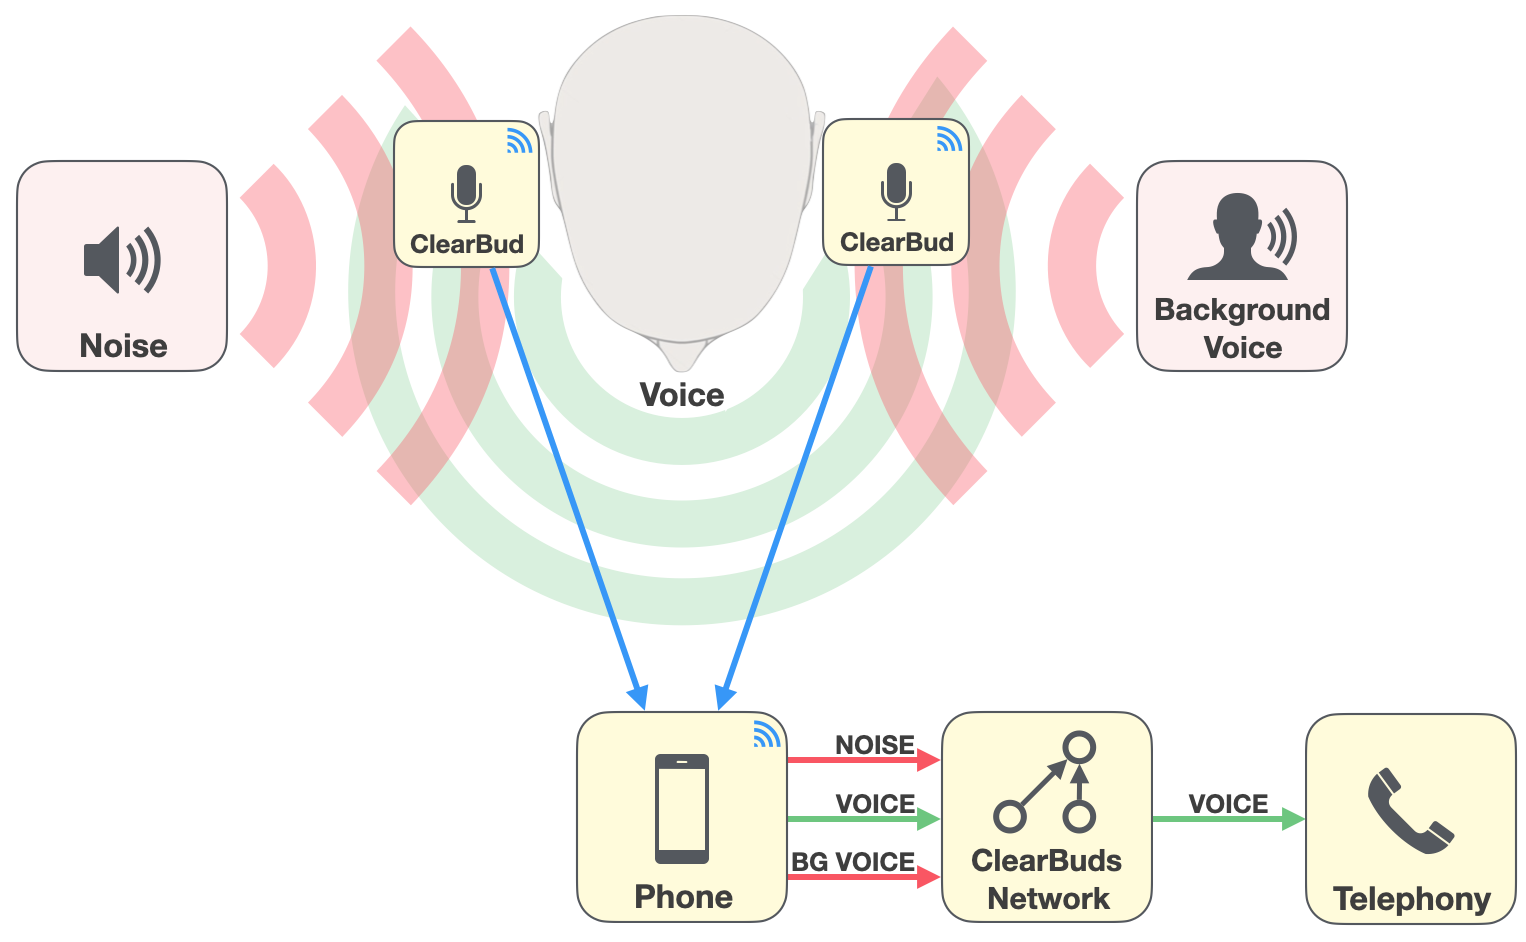
\includegraphics[width=0.75\linewidth]{CB_figures/flow-diagram-6.png}
\vskip -0.1in
\caption{{ ClearBuds Application.  Our goal is to isolate a user's voice from background noise (e.g., street sounds or other people talking) by performing source separation  using a pair of custom designed, synchronized, wireless earbuds.}}
\label{fig:block_diagram}
\vskip -0.15in
\end{figure}


% From a user experience perspective, this would allow a user to not toggle the mute button on call, even when they are not speaking.

%%%%%%%%%%%%%%%%%%%%%%%%%%%%%% DRAFT 4 %%%%%%%%%%%%%%%%%%%%%%%%%%%%%%%%%%%%

With the rapid proliferation of wireless earbuds (100 million AirPods sold in 2020~\cite{airpodssales}), more people than ever are taking calls on-the-go.  While these systems offer unprecedented convenience, their mobility raises an important technical challenge:  environmental noise (e.g., street sounds, people talking)  can interfere and make it harder to understand the speaker.
We therefore seek to enhance the speaker's voice and suppress background sounds using speech captured across the two earbuds. 


Source separation of acoustic signals  is a long-standing problem where the conventional approach for decades has been to perform beamforming using multiple microphones. Signal processing-based beamformers that are computationally lightweight can encode the spatial information  but do not effectively capture acoustic cues~\cite{van1988beamforming,krim1996two,chhetri2018multichannel}.  Recent work has shown that deep neural networks can encode both spatial and acoustic information and hence can  achieve superior source separation  with gains of up to $9$~dB over signal processing baselines~\cite{subakan2021attention,luo2019conv}. However, these neural networks are computationally expensive. None of the existing binaural (i.e., using two microphones) neural networks can  meet the end-to-end latency required for telephony applications or have been evaluated with real earbud data. Commercial end-to-end systems, like  Krisp~\cite{krisp}, use neural networks on a cloud server for single-channel  speech enhancement, with implications to  cost and privacy. % or on edge devices.

%\footnote{The task of enhancing the wearer's  voice is for  telephony and video conferencing applications. This is not to be confused with active noise cancellation (ANC) which cancels out  noise coming to one's ears from an external environment~\cite{mute}.}

We present the first mobile system that uses neural networks to achieve real-time speech enhancement from binaural wireless earbuds.
Our key insight is to treat wireless earbuds as a binaural microphone array,
and exploit the specific geometry -- two well-separated microphones behind a proximal source -- to devise a specialized neural network for high quality speaker separation. In contrast to using multiple microphones on the same earbud to perform beamforming, as is common in Apple AirPods \cite{airpods} and other hearing aids, we use microphones across the left and right earbuds, increasing the distance between the two microphones and thus the spatial resolution. 


{To realize this vision, we need to address three key technical challenges to deliver a functioning, practical system:
\begin{enumerate}
    \item Today's wireless earbuds only support one channel of microphone up-link to the phone. AirPods and similar devices upload microphone output from only a single earbud at a time.  To achieve binaural speaker separation, we need to design and build novel earbud hardware that can synchronously transmit audio data from both the earbuds, and maintain tight synchronization over long periods of time.
    \item Binaural speech enhancement networks have high computational requirements, and have not been demonstrated on mobile devices with data from wireless earbuds. Reducing the network size naively often leads to unpleasant artifacts. Thus, we also need to optimize the neural networks to run in real-time on smart devices that have a limited computational capability compared to cloud GPUs. Further, we need to meet the end-to-end latency requirements for telephony applications and ensure that the resulting audio output has a high quality from a user experience perspective.
    \item Prior binaural speech enhancement networks are trained and tested on synthetic data and have not been shown to generalize  to real data. Building an end-to-end system however requires a network that generalizes to in-the-wild use. 
\end{enumerate}}
    

%Achieving this goal is challenging for three key reasons. First, today's earbuds are not capable of operating in this manner; AirPods and similar devices upload microphone output from only a single earbud at a time.  To achieve binaural speaker separation, we  need to design and build novel earbud hardware that can synchronously transmit audio data from both the earbuds. Second, binaural speech enhancement networks are not lightweight and have not been demonstrated with wireless earbuds. Reducing the network size naively often leads to unpleasant artifacts. Thus, we also need to optimize the neural networks to run in real-time on smart devices that have a limited computational capability compared to cloud GPUs. Further, we need to  meet the end-to-end latency requirements for telephony applications and ensure that the resulting audio output has a high quality from a user experience perspective. {Third, prior binaural  speech enhancement networks are trained and tested  on synthetic data and have not been shown to generalize well to real  data. Building an end-to-end system however requires a network that generalizes to in-the-wild real use.} 

To achieve this system, we make three  technical contributions spanning earable hardware and neural networks. 


\begin{figure}
\vskip -0.1in
\centering
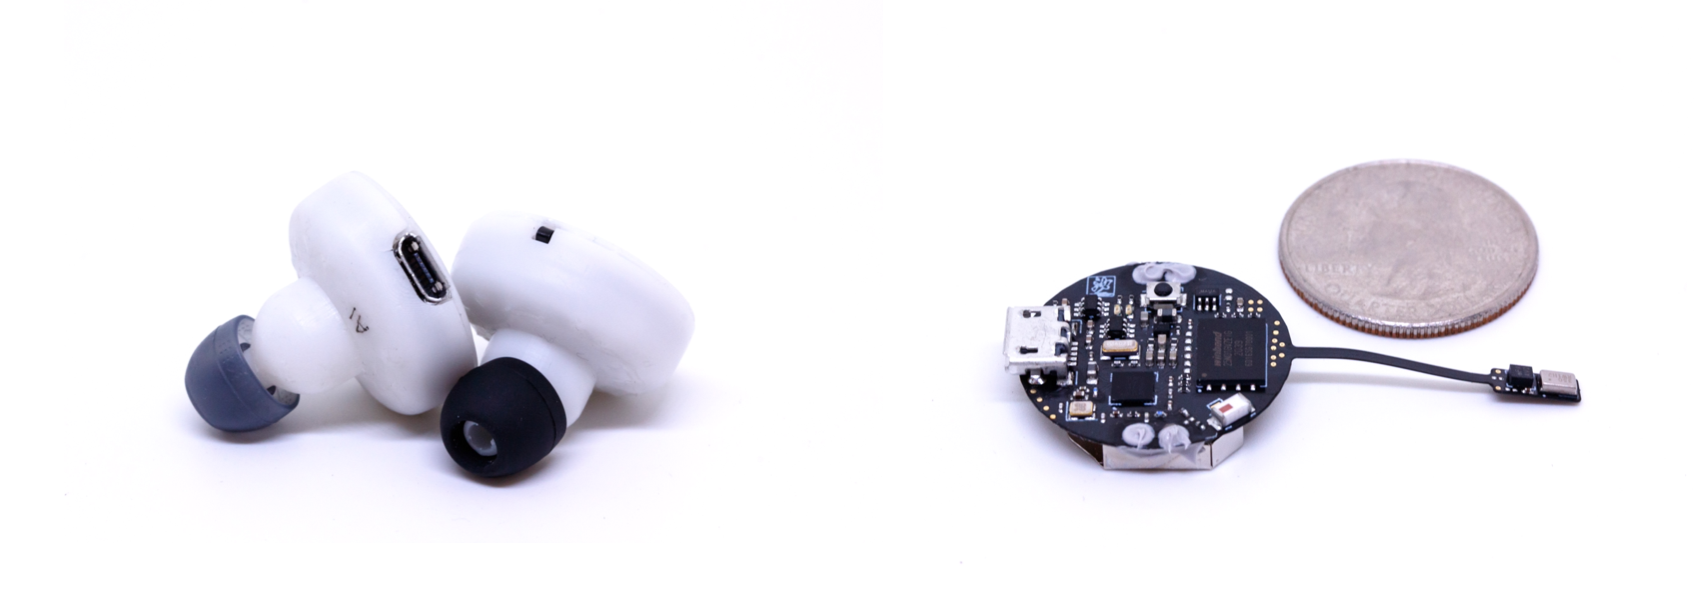
\includegraphics[width=0.5\linewidth]{CB_figures/clearbuds.png}
\vskip -0.15in
\caption{{ClearBuds hardware  inside 3D-printed enclosure and when  placed beside a quarter. }}
\label{fig:earbuds}
\vskip -0.15in
\end{figure}

\squishlist
\item {\bf Synchronized  binaural earables.} We designed a binaural wireless earbud system  (Fig.~\ref{fig:earbuds}) 
capable of streaming two time-synchronized microphone audio streams to a mobile device. This is one of the first systems of its kind, and we expect our  {open-source} earbud hardware and firmware  to be of wider interest as a research and development platform. Existing earable platforms such as eSense~\cite{esense-1}  do not support time-synchronized audio transmission from two earbuds to a mobile device. 
We designed our DIY hardware  using open source eCAD software, outsourced fabrication and assembly ($\$2$K for 50 units), and 3D printed the  enclosures.

\begin{figure}
\vskip -0.1in
\centering
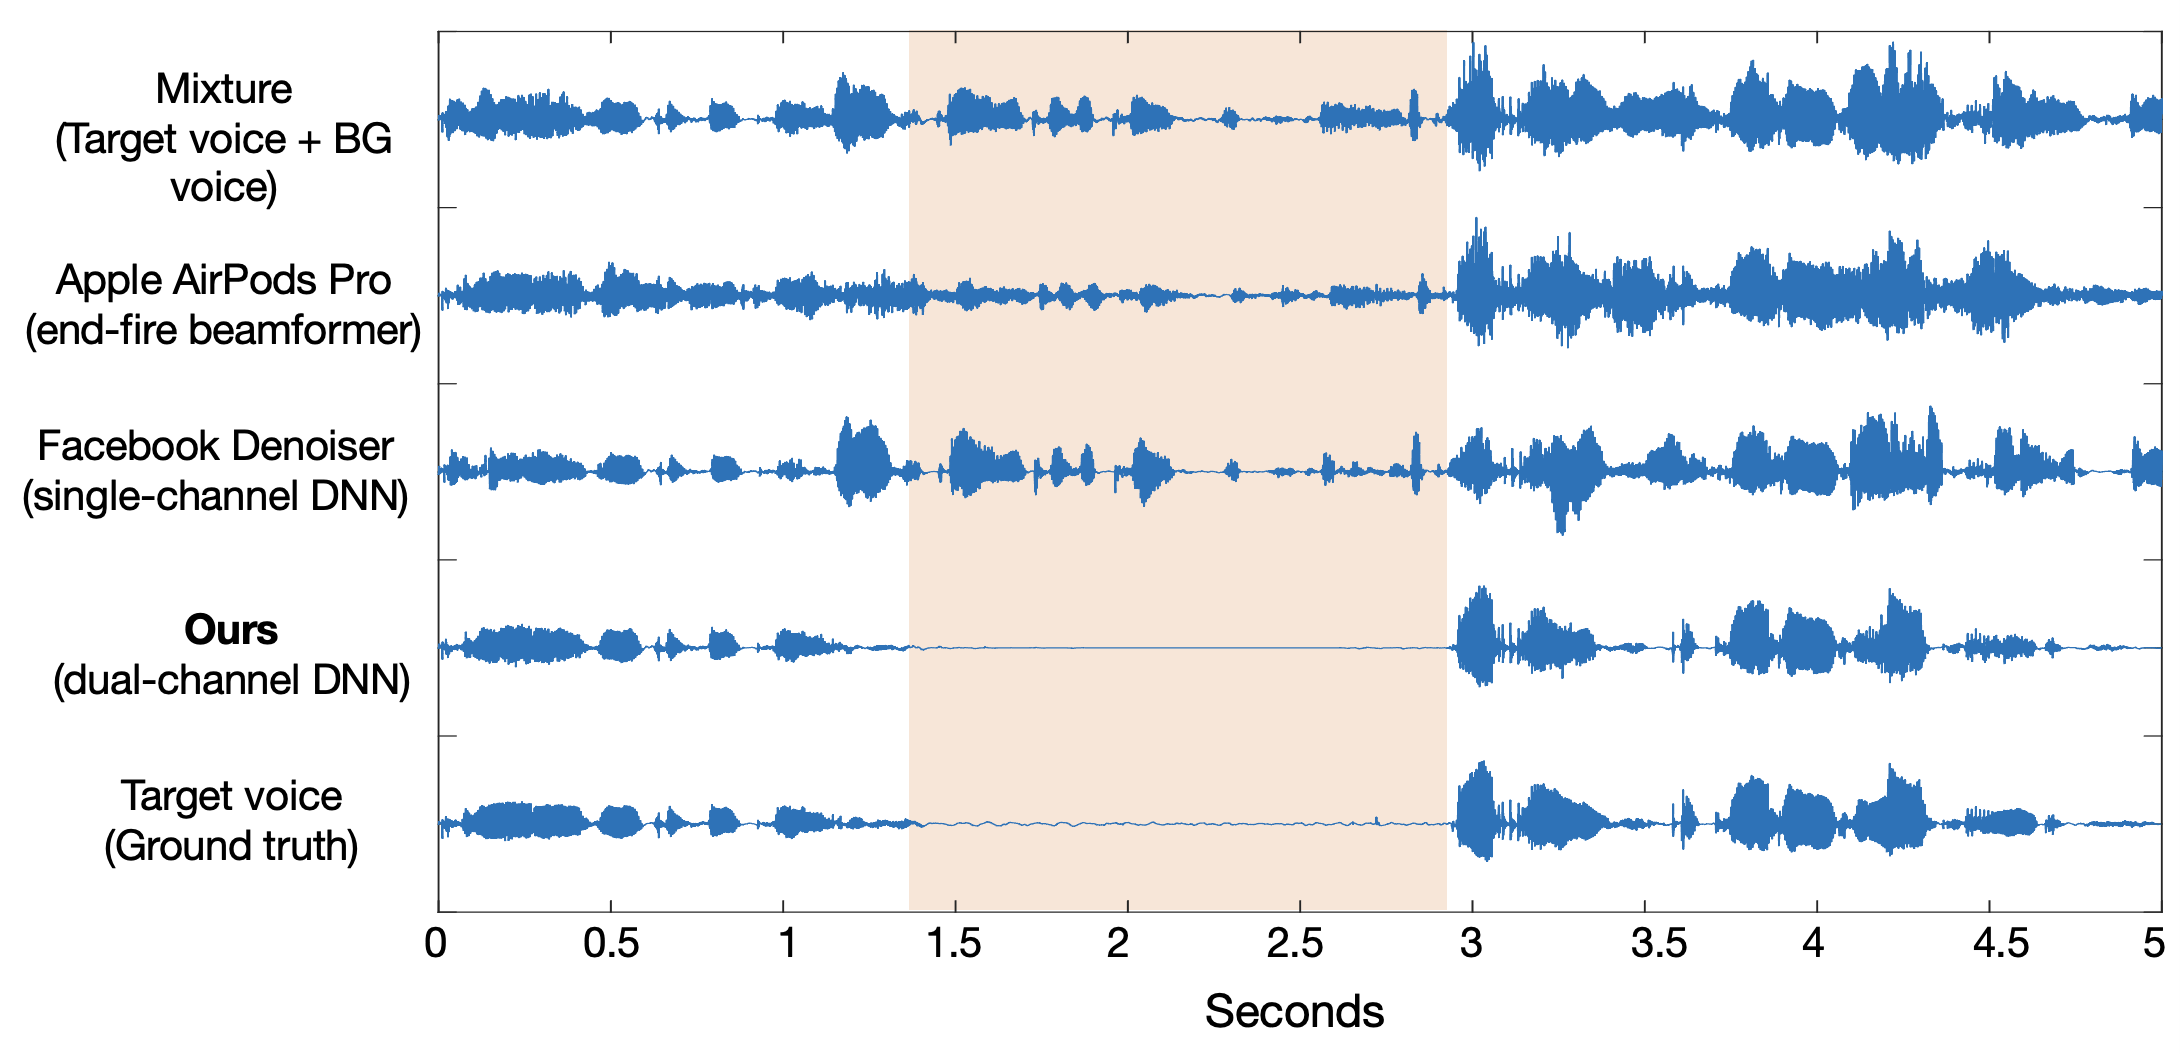
\includegraphics[width=0.75\linewidth]{CB_figures/side_voice_figure_v3.png}
\vskip -0.15in
\caption{{Background voice performance. { We use spatial cues to  separate background voices from the target speaker, even when the background voice is louder than the target voice. This is evident when the target speaker is silent  but background voice continues to talk (highlighted in orange).  Apple AirPods Pro  uses an endfire beamformer to partially suppress  background voice. The mono-channel Facebook Denoiser (Demucs) is unable to suppress the background voice. Clearbud's network  removes the background voice, approaching  ground truth. }}}%Comparing with Airpods:  \textcolor{blue}{\url{https://youtu.be/ZNhbs6lj6a0}} }}} %updated link 2022-05-25 11:48
\label{fig:fig3}
\vskip -0.2in
\end{figure}



\item {\bf Lightweight cascaded neural network.} We introduce a lightweight  neural network  that utilizes binaural input from wearable earbuds to isolate the target speaker. 
To achieve real-time operation, we start with the Conv-TasNet source separation network~\cite{luo2019conv} and redesign the network to achieve a 90\% re-use of the computed network activations from the previous time step for each new audio segment (see~\ref{sec:nn}). While these optimizations make this network real-time, they also introduce artifacts in the audio output {(i.e., crackling, static). Interestingly, these artifacts have little effect on traditional metrics, like Signal-to-Distortion Ratio (SDR), but have a noticeable effect on subjective listening scores (see \ref{sec:mos}). These artifacts however are often visible in a frequency representation of the audio. } To address this, we combine our mobile temporal model with a real-time  spectrogram-based frequency masking neural network. We show that by combining the two networks and creating a lightweight cascaded  network,  we can reduce artifacts and improve the audio quality further. 
\item {{\bf Network training for in-the-wild generalization.} 
Training the network in a supervised way requires clean ground truth speech samples as training targets. This is difficult to obtain in fully natural settings since the ground truth speech is corrupted with background noise and voices. Training a network that generalizes to in-the-wild scenarios also requires the training data to mimic the dynamics of real speech as closely as possible. This includes reverb, voice resonance, and microphone response. Synthetically rendered spatial data is the easiest type of data to obtain, but most different from real recordings, while real speakers wearing the headset in an anechoic chamber provide the best ground-truth training targets, but are the most costly to obtain. Synthetic data can simulate various reverb and multi-path that are not captured in an anechoic chamber. {Our training methodology  uses large amounts of synthetic data simulated in software, small amounts of hardware data with  speakers embedded into a foam mannequin head and small amounts of data from human speakers wearing the earbuds in an anechoic chamber   (see~\ref{sec:datasets}) 
to create a neural network that generalizes to  users and multi-path environments not in the training data. }}

 \squishend

We combine our wireless earbuds and neural network to create ClearBuds, an end-to-end system capable of (1) source separation for the intended speaker in noisy environments, (2) attenuation and/or elimination of both background noises and external human voices, and (3) real-time, on-device processing on a commodity mobile phone paired to the  two earbuds.  Our results show that:
\squishlist
    \item Our binaural wireless earbuds  can stream audio to a phone with a synchronization error less than 64$\mu$s and operate  continuously on a coin cell battery for 40 hours.
    \item Our system outperforms Apple AirPods Pro by 5.23, 8.61, and 6.94~dB  for the tasks of  separating the target voice from background noise, background voices, and a combination of background noise and voices respectively.
    \item Our network has a runtime of 21.4ms on iPhone 12, and the entire ClearBuds system operates in real-time with an end-to-end  latency of 109ms.  For telephony applications, an ear-to-mouth latency of less than 200ms is required for a good user experience \cite{g.114}.
    \item In-the-wild evaluation with eight users in various indoor and outdoor scenarios  shows that our system  generalizes to previously unseen participants and multipath environments,  that are not in the training data.  
    \item In a user study with 37  participants who spent over 15.4  hours and rated a total of 1041  in-the-wild  audio samples, our cascaded network achieved a higher mean opinion score and noise suppression  than both the input speech as well as a  lightweight Conv-TasNet. 
    
    
%    \item Our network can run in real-time on a mobile device with a latency of 155ms on an iPhone 12
\squishend




We believe that this paper  bridges state-of-the-art deep  learning for blind audio source separation and in-ear mobile systems. The ability to perform background noise suppression and   speech  separation could positively   impact  millions of people who use earbuds to take calls on-the-go. By open-sourcing the hardware  and collected datasets, our work may  help kickstart future research among mobile system and machine learning researchers to design  algorithms around wireless earbud data.

    
%The link below shows a system demo:\begin{center}{\textcolor{blue}{{{\url{https://youtu.be/0Hmnc054cow}}}}}\end{center}
    

%%%%%%%%%%%%%%%%%%%%%%%%%%%%%% RANDOM NOTES %%%%%%%%%%%%%%%%%%%%%%%%%%%%%%%%%%%%


% Imagine a world a in 

% They cannot do two channel because of bluetooth reasons

% They are doing beamforming on one device

% What is the first thing that we're doing

% What's novel about the end to end system, it's real time, on the mobile device, using two mics

%%%%%%%%%%%%%%%%%%%%%%%%%%%%%% DRAFT 2 %%%%%%%%%%%%%%%%%%%%%%%%%%%%%%%%%%%%


% Background noise during phone and video calls is a persistent problem that affects people all over the world. Environmental sounds, such as street noises, machinery noises, or other people talking, can be transmitted along with the speaker, which hinders the ability to clearly communicate.

% Speech enhancement is the task of isolating the speaker of interest and suppressing all unwanted background sounds. Recently, there have been many advances in machine learning that attempt to remove these artifacts from a single microphone input. Such systems do not perform well in situations where multiple human speakers are present due to the fact that a single microphone model lacks the spatial information required to isolate the intended speaker. In addition, such systems generally perform worse than those that utilize multiple microphones.  

%  We are particularly motivated by the rise in multi-microphone wearable headphones in everyday settings. Examples include AirPods and PixelBuds, which have become increasingly popular in recent years. Although these devices often employ some amount of directional pickup, via beamforming or microphone design, these mechanisms offer limited attenuation of background noise compared to deep learning methods.
 
%  In contrast to these approaches, we propose a neural network that utilizes binaural input from wearable headphones in order to isolate the target speaker based on both voice and spatial information. Furthermore, we design our network to run real-time on a mobile device and show low latency across a variety of devices. To achieve real-time separation, we use a Temporal Conv-Net based separation network that allows caching of intermediate outputs. When running on streaming input chunks of 50ms, we can re-use 99\% of the computed network activations from the previous time step for each new segment of audio. Experiments show that our network can outperform a number of baselines on both synthetic and real data.
 
%  As a further contribution, we designed a set of wireless earbuds that maintain time synchronization between the microphones at a resolution of 32 microseconds. We built a custom wireless protocol over Bluetooth Low Energy (BLE) to enable synchronized, two-channel microphone streaming to the mobile device. To our knowledge, this is one of the first systems to be able to synchronously stream each microphone channel from each earbud to the mobile phone. This represents a step forward from single earbud beam-forming techniques, which were designed around the fact that current Bluetooth audio protocols only support one microphone channel for uplink. We expect our wireless earbuds to be of wider interest to the spatial audio community as a research and development platform.
 
% %  Because the current Bluetooth hands-free profile (HFP) only supports one microphone for uplink, 
 
% %  This represents a step forward from traditional single-side, on-device beam-forming techniques, and we expect our technique to be of wider interest to the spatial audio community.
 
%  We combine the neural network with our headphones to create a system called ClearBuds, an end-to-end system capable of (1) source separation for the intended speaker in noisy environments, (2) attenuation and/or elimination of both background noises and external human voices, and (3) real-time processing on a pair of wireless earbuds paired with a mobile phone. 







%%%%%%%%%%%%%%%%%%%%%%%%%%%% RANDOM NOTES %%%%%%%%%%%%%%%%%%%%%%%%%%

% For most use cases, speech enhancement systems must run in real-time on the hardware available. This hardware includes both the microphone available as well as the processing hardware. Although many previous works use a single microphone along with a GPU or a laptop CPU,


% In contrast to traditional speech enhancement techniques, we notice that the geometry of the mouth with respect to earbuds allows us to apply an additional geometric heuristic, which then allows us to adapt source separation techniques to speech enhancement. xxxxxx

% In contrast to more general purpose source separation formulations, the key insight is that for speech enhancement on wireless earbuds, the goal is to focus on the voice source  that is approximately equidistant from the two earbuds. 

% To separate the wearer's voice we train a neural network to separate voice sources that are in the center of the microphone array. We use a similar technique as Cone-of-Silence, but do not need the location conditioning variables because the target speaker is always in a known position. xr

% P1
% (1) Succinctly define the problem. Need speech enhancement on earbuds. Focusing on the person who is talking.
% (2) This is useful because people are talking while walking around (buses, streets) with wireless earbuds, existing approaches are not equipped to solve this.

% P2
% Beamforming, why they don't work. 2-3 academic citations, limited because of this reason. 
% On the other hand neural networks have done single channel, but they are limited due to .
% Synthetic data , non causal

% P3
% We built xxx. Key insight to make this realtime is xx. Built system which can wirelessly stream this thing and collected real data.

%%%%%%%%%%%%%%%%%%%%%%%%%%%%%% DRAFT 1 %%%%%%%%%%%%%%%%%%%%%%%%%%%%%%%%%%%%

% \textcolor{red}{Shyam: This history lesson is not required.}
%  In all aspects of our daily lives, the ability for us to hold conversations from one to another anywhere around the world has become an ability that is important in both our personal and work lives. Engineering efforts continue to push the telephony experience by improving voice quality, reducing latency, and eliminating background noise for a better experience. Finally, the advent of telephony has also contributed toward the rapid advancement of audio devices such as wireless earbuds and headsets for both improved voice quality and the ability to take calls hands-free.

% % Improvements in the telephony experience also extend into the video domain. Video calls and video conferencing have been established so that we can now see each other’s faces to further improve the experience of effectiveness of our ability to communicate and collaborate with each other. In the work environment especially, video conferencing has become a necessity for employees and collaborators working from home and working remotely. Indeed, the SARS-CoV-2 (COVID-19) pandemic has only exacerbated this need, as the need for effective video conferencing software (Zoom, Microsoft Teams, Cisco Webex) has become a staple for us to remain effective while we work from home.

% \textcolor{red}{In efforts to continue to improve the telephony experience, engineering innovations are made across both the hardware and software space. For example, digital MEMS microphones have long been preferred to their analog counterparts for noise immunity in wireless audio systems with high frequency radio components.} Today’s phones and wireless earbuds have also taken a step further by adding beam-forming to amplify a speaker’s voice while attenuating external background noise. While the strengths of beam-forming become stronger with distance between two microphones, companies like Apple and Google still integrate dual microphones on their wireless earbuds like AirPods and PixelBuds to gain the benefits of beam-forming microphones. While beam-forming functions well on these edge devices, its ability to attenuate non-broadband-noise fall short. Noises such as loud buses and subways, home appliances, and other background voices persist in the audio uplink during a voice call, disrupting the overall communication experience.

% Recently, developments in the machine learning space have attempted to remove these extremities from a single microphone channel. These networks operate by utilizing spectrogram transformations to learn human voice priors, thus retaining human speech while eliminating other noises. While research continues in the academic space, companies like Krisp have begun to productize this technology so that people can enjoy voice and video calls with background noise removal in the uplink channel. Interest in this technology has also influenced companies like Google, as they recently introduced background noise cancellation on their video conferencing platform, Google Meet.

% While Krisp and Google Meet perform well to isolate human speakers while eliminating background noise, they do not perform well in situations where multiple human speakers are present. This is primarily due to the fact that a single microphone model lacks the spatial information required to isolate the intended speaker in respect to surrounding background voices. This is a nontrivial pitfall, as the ability for these networks to remove noise and background voices in environments such as cafes, call centers, or shared work spaces become weaker.

% To combat this, we introduce and propose ClearBuds, an end-to-end system capable of (1) source separation for the intended speaker in noisy environments, (2) attenuation and/or elimination of both background noises and external human voices, and (3) real-time processing on a pair of wireless earbuds paired with a mobile phone. The basis of our contributions function by integrating both the advances in the wireless earbud ecosystem along with audio source separation networks in the deep learning space. Specifically, we architect and engineer a solution which streams microphone data from both a user’s left and right ear as inputs for our source separation network. With two input channels, our network now attains the spatial information required to eliminate background voices while also isolating the intended speaker, which should be spatially equidistant between a pair of wireless earbuds.

% The contributions of this approach are feasible with our end-to-end system which consists of a pair of wireless earbuds and a mobile phone. Custom firmware is embedded in each earbud which maintains time synchronization between the microphones at a resolution of 32 microseconds. Additionally, a custom wireless protocol is designed to stream the time-synced microphones in real-time to a mobile phone for processing. To our knowledge, this is the first system in which multiple wireless microphones are leveraged to expand upon commercially available background noise cancellation voice technologies (Krisp, Google Meet). Transitively, this is also the first demonstration of streaming both microphones in a pair of wireless earbuds, taking a step forward from traditional single-side, on-device beam-forming techniques. We present comparative results to show that we perform comparatively against non-causal [deep learning model] by xxx dB, while outperforming commercially available models (Krisp) by xxx dB and on-device beam-forming (AirPods) by xxx dB. 


\section{ClearBuds Design}

We first introduce our  lightweight  neural network architecture. We then describe system design  of our hardware platform and our synchronization algorithm. % to ensure time alignment between each ClearBud's microphone.



\subsection{Problem Formulation}
Suppose we have a 2 channel microphone array with one microphone on each ear of the wearer. The target voice is speaking with a signal $s_0 \in \mathbb{R}^{2 \times T}$ in the presence of some background noise $\textbf{bg}$ or other non-target speakers $s_{1..N}$. There may also be multi-path reflections and reverberations $\textbf{r}$ which we would also like to reduce, i.e., $\mathbf{x} = \sum_{i=0}^{N}\mathbf{s}_i + \mathbf{bg} + \mathbf{r}$.  Our goal is then to recover the target speaker's signal, $s_{0}$, while ignoring the background, reverbations, or other speakers. We also must do so in a real-time way, meaning that the a mixture sample $\textbf{x}_t $ received at time $t$ must be processed and outputted by the network before $t + \textbf{L}$ for some defined latency $\textbf{L}$.  We refer to the non-target speakers as "background voices". These background voices may be at any location in the scene, including very close to the target speaker and their angle  can change with time and motion.



\subsection{Neural Network Architecture Motivation}\label{sec:nn}




 %Our target network is approximately causal and runs in real-time on a mobile device.
  {Our network needs to perform in real-time on a mobile device with minimal latency.}
 This is challenging for several reasons. First, the processing device has a much lower compute capacity, especially compared to cloud GPUs. Additionally, the network should separate non-speech noises as well as unwanted speech. To do this, it must learn spatial cues and human voice characteristics. Finally, the resulting output should maximize the quality from a human experience perspective while minimizing any artifacts the network might introduce. 

Our network, which we call \textit{ClearBuds-Net} or \textit{CB-Net}, is a cascaded model that operates in both  time  and frequency domains. The full network architecture is illustrated in Fig.~\ref{fig:network-full} and contains two main sub-components: A dual-channel time domain network called \textit{CB-Conv-TasNet}, and a frequency based network called \textit{CB-UNet}. %Next, we  describe the motivation for each component of the network.


% \textcolor{red}{XXXThis needs to be rewritten. We need tos tart with the network architecutre and then talk about the details of each of the network and show example spectrograms to give the motivation for the frequency masking network.}


% To address this,. Second, the compute device has a much lower memory and compute capacity, especially compared to standard GPUs. To solve this, we use depthwise separable convolutions as described in \cite{howard2017mobilenets}. We also use a temporal convolution network (TCN) that allows caching of intermediate outputs to reduce computation on new packets. Finally, 


\subsubsection{CB-Conv-TasNet}
The first component of separation method is a time domain network that is based on a multi-channel extension of Conv-TasNet \cite{luo2019conv}. This is a network in the waveform domain that  has a  Temporal Convolution Network (TCN) structure, lending itself to a causal implementation with intermediate layer caching \cite{paine2016fast}. We  use depthwise separable convolutions~\cite{howard2017mobilenets} to  further reduce the number of parameters and make the design real-time. We call this network CB-Conv-TasNet since it is an optimized version of the original Conv-TasNet.

A key feature of the time domain approach is that it can easily capture spatial cues in the network. In our application, the desired source is always physically between  two  microphones, thus the voice signal will reach the microphones roughly at the same time. In contrast,  background or other speakers are typically not temporally aligned and will reach one microphone earlier or later. By feeding two time synchronized channels into the neural network, this spatial alignment of the sources can be learned from time differences in the signal. This is similar to a delay-and-sum beamforming effect, except the sum is replaced with a deep network. %Although a similar spatial separation approach was demonstrated in \cite{jenrungrot2020cone}, this spatial approach in the time-domain alone is not sufficient to produce quality output given the resource constraints of the computing device. NOT SURE WHAT THIS IS ADDING EXCEPT FOR HIGHLIGHT THIS PRIOR WORK.

\begin{figure*}
%\vskip -0.5in
\centering
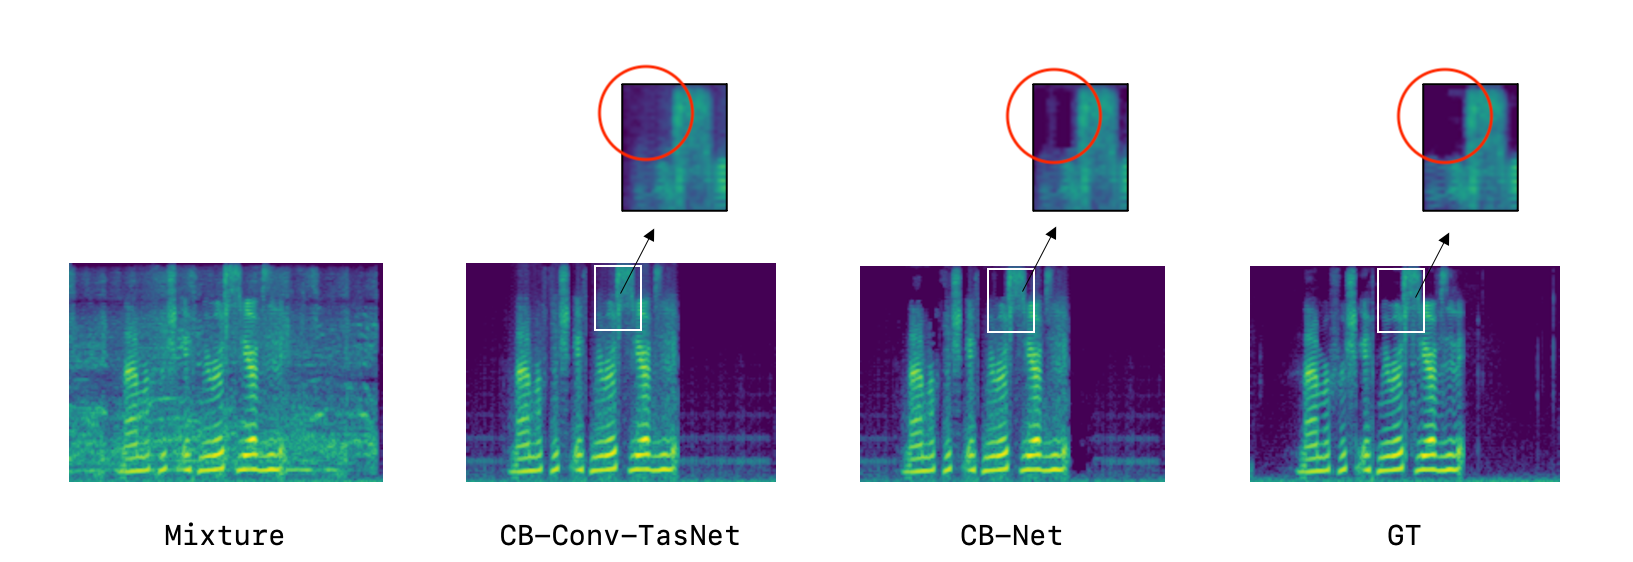
\includegraphics[width=0.75\linewidth]{CB_figures/spectrogram_motivation2.png}
\vskip -0.15in
\caption{{The spectrograms above show the motivation behind a combined time and frequency domain method. The output of the time-domain component, CB-Conv-TasNet, contains artifacts, particularly at high frequencies. Although subtle, these artifacts are perceptible by human listeners. CB-Net is able to reduce these artifacts by using a frequency-domain network (CB-UNet) that masks unwanted frequencies.}}
\vskip -0.2in
\label{fig:spectrogram-motivation}
\end{figure*}

\subsubsection{CB-UNet}
 {The output of our lightweight CB-Conv-TasNet often contains audible artifacts (i.e., crackling, static) that reduce the listening experience. Interestingly, these artifacts have little effect on traditional metrics, like Signal-to-Distortion Ratio (SDR), but have a noticeable effect on subjective listening scores (see \ref{sec:mos}). These artifacts are often visible in a frequency representation of the audio.  Fig.~\ref{fig:spectrogram-motivation} shows how  CB-Conv-TasNet alone contains noticeable artifacts when compared to the ground truth. To address this, we cascade a lightweight causal UNet \cite{ronneberger2015unet} which operates on the mel-scale spectrogram of the input audio. This network, which we call CB-UNet, produces a binary mask which is applied to the output of CB-Conv-TasNet. The combined output, shown in Fig.~\ref{fig:spectrogram-motivation} as CB-Net,  reduces these artifacts. The mean opinion scores in our evaluation  shows the strength of the cascaded CB-Net when compared to the time-domain component only.}

\subsection{Neural Network Detailed Description}

%Here, we describe details of our  network architecture.

\subsubsection{CB-Conv-TasNet}
The input to the network is a binaural mixture given by $\textbf{x} \in \mathbb{R}^{2 \times T}$. The first step is an encoder that transforms the mixture $\textbf{x}$ into $\mathbb{R}^{N \times T/L}$ with a 1D convolution of size $L$ and stride $L$. This is followed by a ReLU layer. The encoder's outputs are next fed into a temporal convolution network that consists of stacks of 1-D convolutions with increasing dilation factors. We use 14 convolution layers with dilation factors of 1,2,4,..,64 repeated twice, with a ReLU nonlinearity and skip connection after each convolution. The encoder output is multiplied with the output of the temporal conv-net, before being fed through a fully connected Decoder layer which transforms the output back into $\mathbb{R}^{2 \times W}$. %We describe window size  $W$ in the next sections. %\textcolor{red}{You can also refer to figure (need to insert) for a visual layout of the network.}



In a real-world implementation, we do not have access to the full waveform, but only packets of data at a time. Furthermore, we must process these packets with limited access to future input samples. Given  15.625 kHz sampling rate, we choose to process packets of 350 samples at a time (22.4ms), which is our  window size $W$. We also use $2W$, or 700 samples of lookahead time (44.8ms) and 1.5s of past samples. Since we have no padding in the temporal convolution net, the network starts with this large temporal context and outputs exactly $\mathbb{R}^{1 \times W}$ samples, corresponding to the desired output for our input packet of $W$ samples. When we receive the next packet of size $W$, all intermediate activation from the encoder and temporal conv-net can be shifted over by $W / L$ samples and re-used. We chose $L = 50$, but any divisor of $W$ would work. Re-using intermediate outputs from previous packets saves over $90\%$ of the compute time for a new packet in our network. %These ideas of caching causal convolutions has been discussed in previous work such as \cite{paine2016fast}. %https://arxiv.org/pdf/1611.09482.pdf%


\begin{figure}
%\vskip -0.1in
\centering
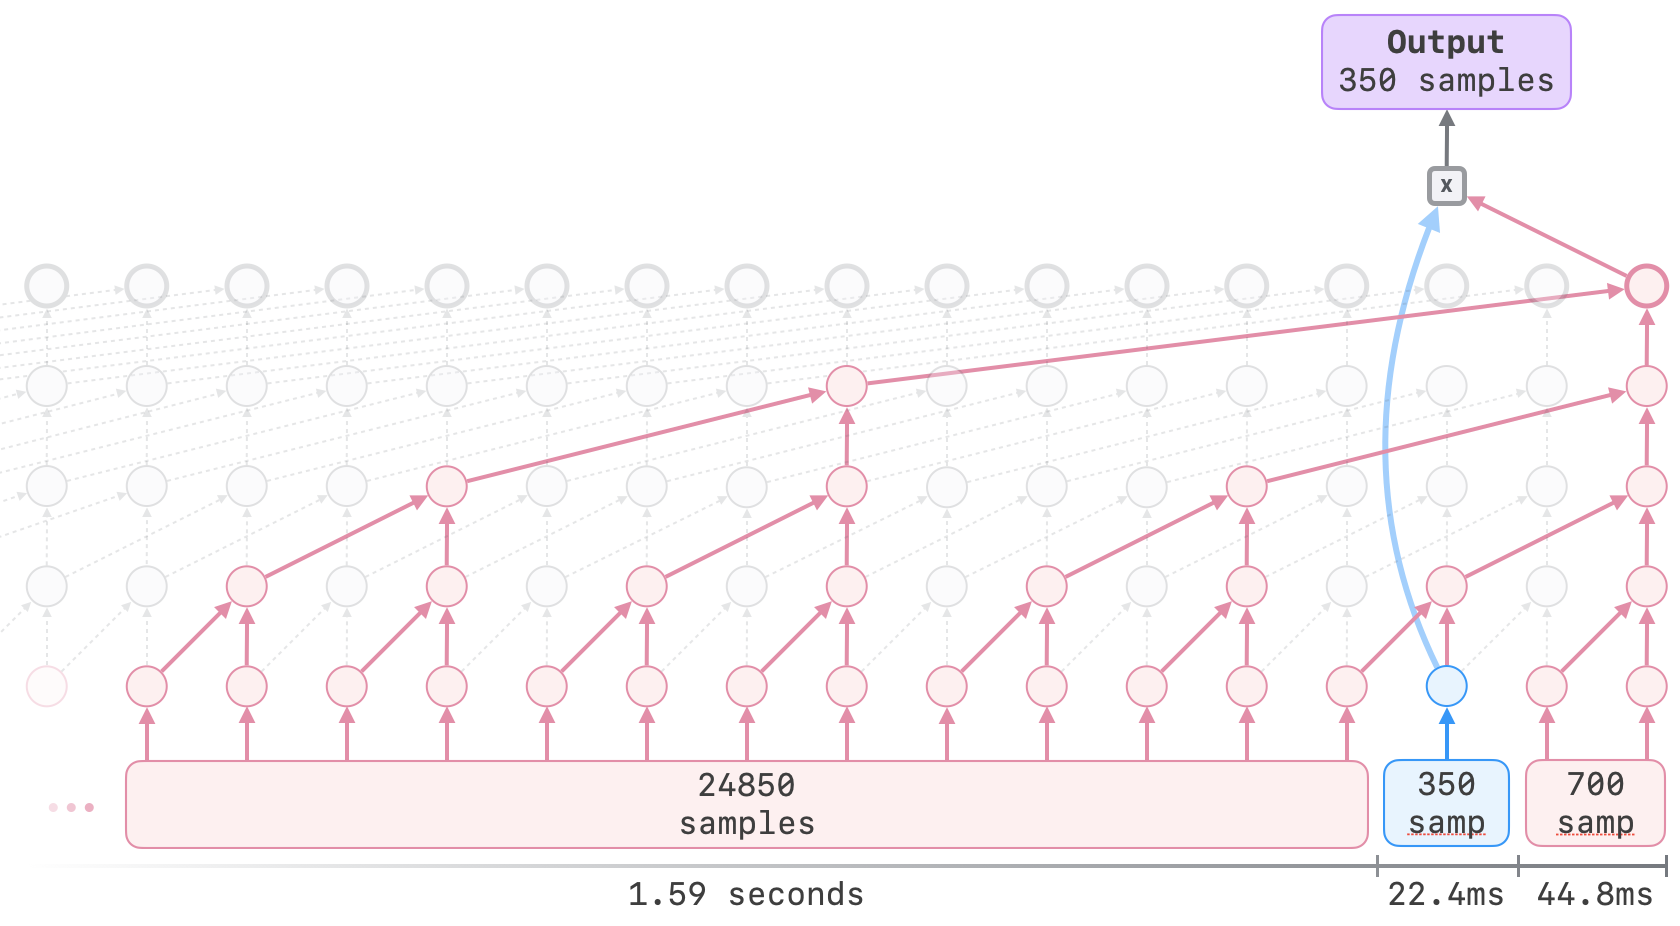
\includegraphics[width=0.75\linewidth]{CB_figures/network-3.png}
\vskip -0.15in
\caption{ CB-Conv-TasNet, the time-domain component of CB-Net. Given a packet of 350 samples (22.4ms) highlighted in blue, we use 1.5s of past input and 44.8ms of future input to output the separation results. Our caching scheme works as follows: When we receive a new 350ms samples, all intermediate activations (circles in the diagram) slide to the left, and we compute only the rightmost column of outputs.}
\label{fig:network}
\vskip -0.3in
\end{figure}

\subsubsection{CB-UNet}

The frequency domain network is a mono-channel network that outputs a binary mask for each time-frequency bin. The input $\textbf{x} \in \mathbb{R}^{1 \times T}$ is a summation of the binaural left and right channel, which is the equivalent of a broadside beamformer. We first run a STFT, which is a mel-scale fourier transform with hop size of $350$, a window size of  $1024$ including zero padding on the edges, and a $128$ bin mel-scale output. The network input is a spectrogram of $64$ time bins and $128$ frequency bins, corresponding to a receptive field of $22400$ samples, or $1.43s$. In order to maintain the causality requirement, we use the same lookahead strategy as the time-domain network where we allow $700$ samples of lookahead for a target packet of $350$ samples. The UNet architecture contains 4 downsampling and upsampling layers, starting with 64 channels and doubling the number of channels at each subsequent layer. The downsampling layers contain a depthwise separable convolution followed by a $2 \times 2$ max pooling, and the upsampling layers contain a depthwise separable convolution followed by a transposed convolution for upsampling. The output is a sigmoid function, which is then thresholded to return a binary mask in $[0, 1]^{128 \times 64}$.  When outputting a spectrogram mask on an $\mathbb{R}^{128 \times 64}$ input, we predict a mask over the entire input even though we only need the output for a specific slice of $350$ samples, or a $\mathbb{R}^{128 \times 1}$ mask. Further optimizations could be made by caching intermediate outputs or only computing the mask for the target samples. However CB-UNet's run-time  was so small compared to the rest of the network that these optimizations were not  necessary.


\subsubsection{Combining the Outputs}
At each time step, the output of CB-Conv-Tasnet is an audio waveform in $x \in \mathbb{R}^{1 \times 350}$, and the output of CB-UNet is a spectrogram mask in $\textbf{M} \in \mathbb{R}^{128 \times 64}$. We run the same fourier transform on the buffered conv-tasnet outputs to produce a spectrogram $\textbf{X} \in \mathbb{R}^{128 \times 64}$. Our output can then be computed by $iSTFT(\textbf{M} \otimes \textbf{X})$.
 Our empirical results show that  this gives the best results compared to other methods such as ratio masking.
%Previous work \cite{zhao2018sound} has shown the benefits of binary masking for spectrogram based separation, and

\subsubsection{Training}
CB-Conv-TasNet is trained with an $L1$-based loss over the waveform along with the multi-resolution spectrogram loss. Formally, provided $s_{0}$ is our target speaker and $x'$ is the output from the network, our loss is:
\begin{equation*}
    L(s_{0}, x') = \left\Vert s_{0} - x' \right\Vert_1 \\ + L_{sc}(s_0, x') + L_{mag}(s_0, x')
\end{equation*}
\begin{equation*}
L_{sc}(s_0, x') = \frac{\left\Vert STFT(s_0) - STFT(x')\right\Vert_F}{\left\Vert STFT(s_0)\right\Vert_F}
\end{equation*}
\begin{equation*}
L_{mag}(s_0, x') = \left\Vert \log(STFT(s_0) - \log(STFT(x'))  \right\Vert_1
\end{equation*}
STFT denotes the magnitude of the short time Fourier transform, and $F$ denotes the Frobenius norm. $L_{sc}$ and $L_{mag}$ represent  spectral convergence and magnitude losses, which  gave better results than L1 loss alone.

For training CB-UNet, for each time frequency bin, the training target $\textbf{M}$ is 1 if the target voice is the dominant component, and 0 otherwise. Formally, $\textbf{M}(f, t) = [\textbf{S}_{0}(f, t) \geq \textbf{S}_{i}(f, t)], \;\; \forall i = (1..n)$. The network is then trained with the binary cross entropy of the output compared to the target mask.


\subsubsection{Hyperparameters and Training Details}

 We use a learning rate of $\SI{3e-4}{}$ along with the ADAM optimizer  \cite{kingma2014adam} for training the network. The network was trained on a single Nvidia TITAN Xp GPU. Because of the small size of the network, training could be completed within a single day and generally required $\approx$50 epochs to reach convergence.As an additional data augmentation step we make the following perturbations to the data: High-shelf and low-shelf gain of up to $\SI{2}~{dB}$ are randomly added using the \texttt{sox} library.

\subsection{Synchronized wireless earbuds}

\begin{figure}
\vskip -0.1in
\centering
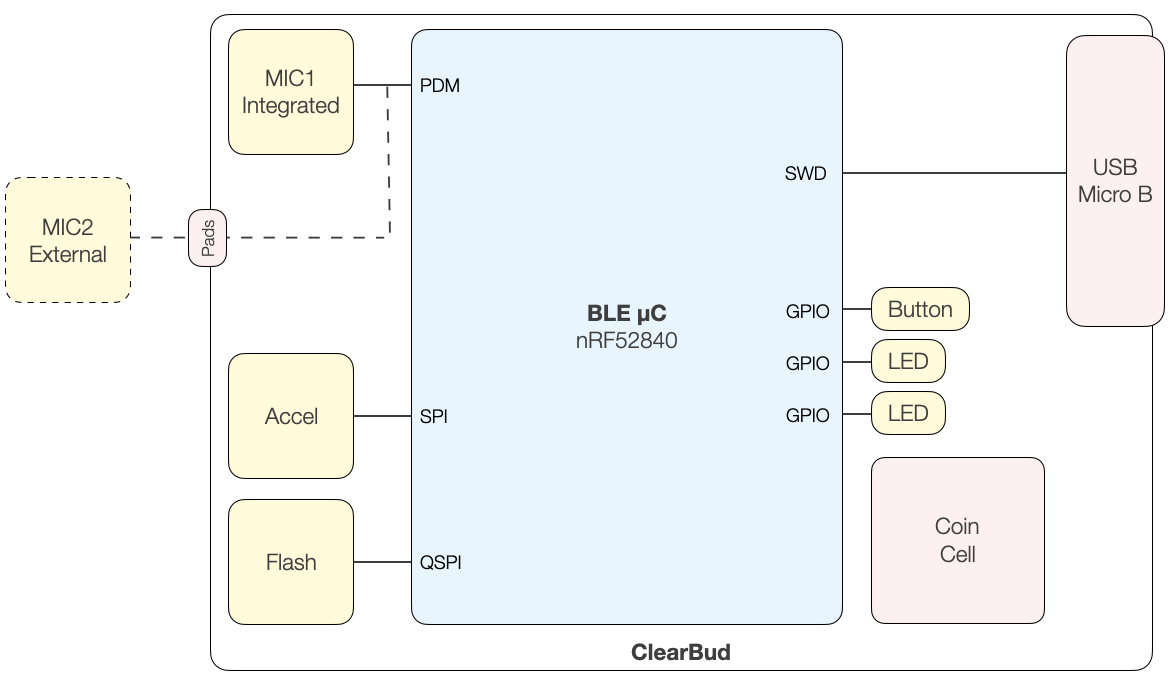
\includegraphics[width=0.75\linewidth]{CB_figures/ClearBud-Block-Diagram.png}
\caption{Hardware Block Diagram. Each ClearBud integrates a PDM microphone, accelerometer, flash, and coin cell battery. Buttons and LEDs are used for interfacing with the device, and a USB port is used for programming and debug.}
\vskip -0.2in
\label{fig:block-diagram}
\end{figure}

\label{sec:system}
 We seek to capture speech from the target speaker's mouth which sits on the sagittal plane roughly  equidistant to the ears. Given an ear-to-ear spacing of 17.5cm, to effectively isolate this central plane we require a distance precision on the order of a few centimeters.
An interaural time difference of 100$\mu$s  would correspond to source maximally 3.43 cm off this central plane, therefore we target a synchronization accuracy under 100$\mu$s.


\begin{figure*}
\vskip -0.1in
\centering
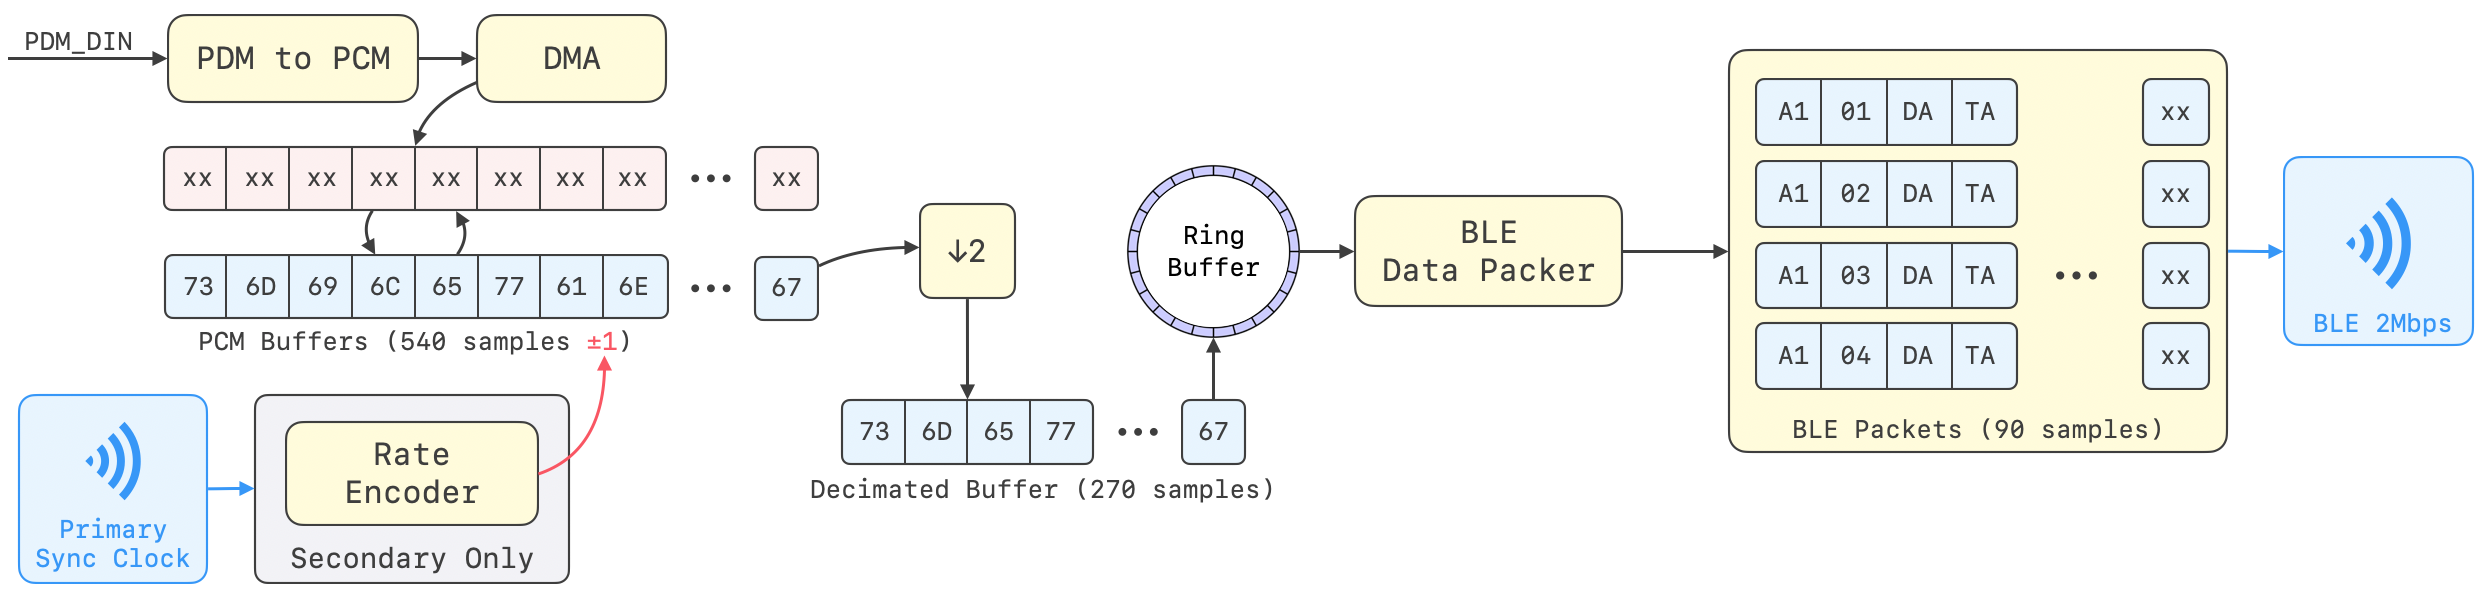
\includegraphics[width=0.85\linewidth]{CB_figures/mic-pipeline-2.png}
\vskip -0.1in
\caption{Time Sync Design. The primary ClearBud broadcasts a sync clock over the air. The secondary ClearBud then uses the sync clock to rate encode, by increasing or decreasing the size of its local PCM buffer.}% Both ClearBuds then decimate these buffers down by a factor of 2, and fill up a ring buffer.} %Finally, each BLE packet gets prepended with a sequence number and then gets transmitted to a host device. }
\label{fig:sync}
\vskip -0.15in
\end{figure*}


\subsubsection{Hardware}  Our  custom hardware design contains  a %support for up to two 
pulse-density modulated (PDM) microphone (Invensense ICS-41350) and a Bluetooth Low Energy (BLE) microcontroller (Nordic nRF52840).\footnote{For future research applications, an ultra low-power accelerometer (Bosch BMA400), a 1Gbit NAND flash for local data collection (Winbond W25N01GVZEIG), and support for speaker and an additional microphone are included.} The system is powered off of a CR2032 coin cell battery and programmed via SWD over a Micro-USB connector.  Each ClearBud has an integrated PDM microphone set to a clock frequency of 2MHz. With an internal PDM decimation ratio of 64, this provides us a sampling frequency of 31.25kHz. As most HD voice applications and wideband codecs are limited to 16kHz~\cite{voicecodecs}, we decimate further in firmware by a factor of 2, giving us a final sampling frequency of 15.625kHz.

Two 16-bit 180 sample size Pulse-Code Modulation (PCM) buffers are round-robined: one is filled with incoming PCM data while the other is processed. The DMA is responsible for both clocking in the PDM data and converting it into PCM. One buffer is always connected to the DMA, while the other is freed for processing for the rest of the data pipeline. When the buffer connected to the DMA fills, the buffers switch roles and we begin processing data on the newly freed buffer, and connect the other buffer back to the DMA. With this design we always have a continuous PCM stream to operate on.
Both ClearBuds transmit the PCM microphone data to a mobile phone for input into our neural network. To maximize throughput, we use the highest Bluetooth rate and packet sizes supported by iOS, which is 2Mbps and 182 bytes, respectively. We design a lightweight wireless protocol where the first 2 bytes represent a monotonically-increasing sequence number, while the other 180 bytes are reserved for the 16-bit PCM audio samples. The sequence number is used on the  phone so that we can zero-pad PCM data in the occasional event that a packet is dropped either over-the-air or by the radio hardware. This zero-padding keeps the left and right microphone data aligned on the host side in areas of poor radio performance or interference in the environment.

%\subsubsection{Fabrication} 
The hardware schematic and layout for ClearBuds was designed using the open source eCAD tool KiCad. A 2-layer flexible printed circuit was  fabricated and assembled by PCBWay. The 3D printed enclosures were designed using AutoDesk Fusion 360 and printed with a Phrozen Sonic Mini   using  a liquid resin fabrication process.   The MEMS microphone sits behind the lid on the earbud's outer surface.
A single button on the enclosure  provides access to turn on and off the earbuds.

% The sequence number is used on the mobile phone so that we can zero-pad PCM data in the occasional event that a packet is dropped either over-the-air or at the radio hardware layer. This zero-padding keeps the left and right microphone streams aligned on the host side in areas of poor radio performance or interference. However, this is not sufficient to maintain synchronization within 100$\mu$s. We must also account for clock drift between our earbuds. MK: This sounds worse, as if this is the foundation for the sync and clock drift is the secondary feature.





%%Our system architecture revolves around the design of two microphones placed in each user's ear. We choose this design for two reasons. First, it allows us to leverage the spatial data of our desired voice being centered between the mics, while background noise has a higher likelihood of arriving off-center. Second, this configuration allows us to be directly applicable to devices in the hearable sector.

%One hurdle that needs to be overcome, is synchronizing the audio input from both wireless microphones so that our network can properly leverage the TDOA between the audio streams.

%  https://devzone.nordicsemi.com/nordic/short-range-guides/b/bluetooth-low-energy/posts/wireless-timer-synchronization-among-nrf5-devices


\subsubsection{Microphone synchronization} Three components are necessary for maintaining microphone synchronization: (1) As each of our earbuds has its own local clock source, we need to establish a common clock between them so that they have the same reference of time, (2) a synchronized startup so each earbud starts recording from their respective microphone at the exact same time, and (3) a rate encoding scheme to control the earbud's sampling rate to match each other. 

In our system, each earbud has its own respective 32MHz clock source with a total +/- 20ppm frequency tolerance budget. So, in the worst case scenario, the earbuds will have 2.4 milliseconds of drift each minute. We  use the  Nordic's TimeSlot API \cite{timeslot}, which grants us access to the underlying radio hardware in between Bluetooth transmissions. This provides us a transport to transmit and receive accurate time sync beacons \cite{wireless-timesync}. Each ClearBud keeps a free-running 16MHz hardware timer with a max value of 800,000, overflowing and wrapping around at a rate of about 20~Hz. One ClearBud is assigned as the timing master while the other ClearBud will synchronize its free-running timer to the master's.  The primary ClearBud (timing master) transmits time sync packets at a rate of 200~Hz. These packets contain the value of the free-running timer at the time of the radio packet transmission. When the secondary ClearBud receives this packet, it can then add or subtract an offset to its own free-running timer for a common clock. %This allows ClearBuds to maintain an accurate common clock. 

Once each ClearBud is connected to the mobile phone, the phone sends a \verb|START| command to both ClearBuds over BLE. Each ClearBud contains firmware which arms a programmable peripheral interconnect (PPI) to launch the PDM bus once the 16MHz free-running timer wraps around at 800,000. By using this method, we bypass the CPU and trigger a synchronized startup entirely at the hardware layer. One caveat is that the mobile phone could write to one ClearBud right \textit{before} its clock wraps around at 800,000, and the other ClearBud right \textit{after} it wraps around at 800,000. With a clock that wraps around at 20Hz, this would trigger a mismatched startup and cause an alignment error of 50ms. To correct for this, each ClearBud reports its common clock timer value to the phone once it has received the \verb|START| command. The phone can then remove the first 781 audio samples (781 samples / 15.625kHz = 50ms) if one ClearBud started streaming 50ms before the other.

The final component to keeping the audio streams aligned is to create a rate encoding scheme between the ClearBuds. With the time sync beacons from the primary ClearBud, the other ClearBud now has both its local clock and the common clock (primary ClearBud's local clock). With these two clocks, the secondary ClearBud can identify how much faster or slower its PDM clock is running in relation to the primary ClearBud. We note that with a 2MHz PDM clock and a PDM decimation ratio of 64, each audio sample occupies 32~us. The non-primary ClearBud can then add or remove a sample to its PDM buffer every time the difference between the clocks exceeds a multiple of 32~us. By doing this, the secondary ClearBud ensures that its PDM buffer starts filling up at the exact same time as the primary ClearBud's PDM buffer, with a tolerance of 32 us. 
% \subsubsection{Hardware evaluation} \textcolor{red}{This should go to the evaluation. Have to talk about this...} In order to validate our synchronization firmware, we place both ClearBuds roughly equidistant from a speaker. A click tone is played every 15 seconds for 5 minutes, and recorded on both ClearBuds with time sync disabled and enabled. We calculate the sample error on each recorded click.
% %, and convert it into time error with a sampling rate of 15.625kHz.
% Figure ~\ref{fig:sync} shows the synchronization validation results across this experiment. We can see that with time sync enabled, the sample error never exceeds 1 sample at 15,625 kHz, or 64 $\mu$s.

% Finally we evaluate the power consumption of the ClearBuds hardware. We measure current consumption by powering our system through its Micro-USB port with a power supply, which goes through the same power path as our coin cell battery. We set our power supply voltage to 3V and set a maximum current output of 300mA, to reflect the internal 10 ohm resistor of a CR2032 battery. While streaming microphone data, we measure current consumed to be between 5-6mA. With the CR2032's nominal capacity of 210mAh, this translates to 35-42 hours of streaming  operation.

%\begin{figure}
%\vskip -0.1in
%\centering
%\includegraphics[width=1\linewidth]{CB_figures/mic-pipeline.png}
%\caption{\small{Microphone Data Pipeline}}
%\label{fig:mic_pipeline}
%\end{figure}

%[SHOW TIME SYNC PLOT]

%Two plots: Sine wave with time sync ON and sine wave with time sync OFF
%How to best represent drift on a graph? (5, 10, 15, 30, 60min?)

\section{Training methodology} \label{sec:datasets}
%Designing a network that generalizes to in-the-wild settings requires carefully choosing the training methodology.  Training the network requires clean ground truth speech samples as supervised learning targets, which is difficult to achieve in in-the-wild settings since the groundtruth speech is corrupted with background noise and voices. Therefore, our data collection is based on the mix-and-separate framework \cite{zhao2018sound}, where clean speech and noise samples are recorded separately and combined randomly to form noisy mixtures. %The network then learns to predict the clean speech given the noisy mixture.  Here, we describe how  clean ground truth samples and noisy mixtures are generated to train the network. The network is jointly trained on all these  datasets.

Training the network in a supervised way requires clean ground truth speech samples as training targets. This is difficult to obtain in fully natural settings since the ground truth speech is corrupted with background noise and voices. Training a network that generalizes to in-the-wild scenarios also requires the training data to mimic the dynamics of real speech as closely as possible. This includes reverb, voice resonance, and microphone response. Synthetically rendered spatial data is the easiest type of data to obtain, but most different from real recordings, while real speakers wearing the headset in an anechoic chamber provide the best ground-truth training targets, but are the most costly to obtain. Synthetic data can simulate various reverb and multipath that are not captured in an anechoic chamber. We adopt a hybrid training methodology where we first train on a large amount of synthetic data and fine-tune on real data recorded with our hardware. Our training method is based on the commonly used mix-and-separate framework \cite{zhao2018sound}, where clean speech and noise samples are recorded separately and combined randomly to form noisy mixtures. Our  results  show that our network trained this way generalizes to naturally recorded noisy data in  real-world environments.

{\bf Synthetic data.}  This type of data is the easiest to obtain, since a wide variety of voice types and physical setups can be generated instantly. Many machine learning baselines, e.g., \cite{luo2020endtoend, jenrungrot2020cone, tzirakis2021multichannel}, only train and evaluate on synthetic data generated in this manner. To generate the synthetic dataset, we create multi-speaker recordings in simulated environments with reverb and background noises. All voices come from the VCTK dataset \cite{vctk} (110 unique speakers with over 44 hours), and background sounds come from the WHAM! dataset \cite{wham}, with 58 hours of recordings from a variety of noise environments such as a restaurant,  crowd,  and music.

To synthesize a single example, we create a 3 second mixture as follows: two virtual microphones are placed 17.5~cm apart, which is the average distance between human ears \cite{RISOUD2018259}. The target speaker's voice is placed  at the center between the two virtual microphones, and a second voice is placed randomly between $1$ and $5$ meters away and at a random angle. A randomly chosen background noise is also placed in the scene. We then simulate room impulse responses (RIRs) for a randomly sized room using the image source method implemented in the pyroomacoustics library \cite{allen1979image, scheibler2018pyroomacoustics}. The room is rectangular with sides randomly chosen between 5 and 20 meters, and the RT60 values are randomly chosen between 0 and 1 second. All signals are convolved with the RIR and rendered to the two channel microphone array. The volumes of the background are randomly chosen so that the input signal-to-distortion ratio is roughly between -5 and 5 dB. For training, we use 10,000 mixtures generated in this manner.
% \textcolor{red}{XXXTHE ABOVE IS NOT A COMPLETE DISCRIPTION OF WHAT WAS DONE AND CANNOT BE USED TO REPLICATE. HERE IS AN EXAMPLE. To gather a large amount of training data, we use software to simulate random reverberate noisy rooms using the image source model~\cite{scheibler2018pyroomacoustics}. The rooms are simulated using absorption rates of real materials and a maximum RT60 of 500~ms. By default, we use a virtual 6-mic circular array with a radius of 5~cm. The distance between the virtual speakers and the microphone array is at least 0.8~m, and the direction of arrival differences of the speakers are at least $10^{\circ}$. The input direction is modeled as the groundtruth plus a random error less than $5^\circ$ simulating the gaze tracking measurement error \cite{sipatchin2020accuracy}.  We place virtual speakers at random locations within the room playing random speech utterances from the VCTK dataset~\cite{veaux2017cstr}, meanwhile simulating diffused noise from the MS-SNSD dataset~\cite{reddy2019scalable} and WHAM! dataset~\cite{wichern2019wham}. The combined speech power to noise ratio is randomized between $[5, 25]$~dB. 10\%, 40\%, 40\%, 10\% of the generated clips consists of 1-4 speakers, respectively, and we apply random gain within $[-5, 0]$~dB to each speaker. We guarantee that there exists speech utterance overlap for 2-4 speaker scenarios. We render the synthetic audio and generate 4s clips. We generate a total of 8000 clips as training set, 400 clips as validation set, and 200 clips as test set. No speech clips or noise has appeared in more than one of these three sets. }

{\bf Hardware data. } While a large amount of synthetic data can be easily rendered to train the network, it does not contain characteristics such as the microphone response of physical hardware and imperfections in the time-of-arrival. To address this, we also train on a set of recorded voice samples from our earbuds. We set up a foam mannequin head with an  artificial mouth speaker (Sony SBS-XB12) that plays VCTK samples as the spoken ground truth. For background voice recordings, the speaker is placed in varying locations within a one meter radius of the foam head. Physically recorded background noise is provided by binaural version of the WHAM! dataset \cite{wham}, which was recorded in real environments using a binaural mannequin like ours. We record 2 hours each of clean speech, and background voices. 2000 random mixtures are then created for training.

{\bf Human data.} The spoken hardware data above still does not contain natural voice resonance since it is played out of an electronic speaker. Furthermore, the background sounds recorded by a mannequin wearing earbuds still misses some of the physical filtering of the human body. To better capture desired output of real scenarios, we collect a ground-truth speech dataset in an anechoic chamber with human speakers (5 male, 4 female) and a noise dataset in real environments with human listeners. For the voice data, each human speaker wore our ClearBuds prototypes, and uttered 15 minutes of text from Project Gutenberg in the anechoic chamber. The purpose of this anechoic data is to provide clean training targets for the network, modelling the resonance of human speakers wearing our hardware.
For the real world  noise dataset, individuals wore ClearBuds and recorded various noisy scenarios such as washing dishes, loud indoor/outdoor restaurants, and busy traffic intersections. 2000  random mixtures of clean voice and recorded noise were generated for this dataset. 

Our network is jointly trained using all these  datasets. Note that  testing and evaluation is  done  {\it outside} the anechoic chamber. 

% Finally, we collect an evaluation set with 2 human speakers (1 male, 1 female) in 2 noisy environments, both unseen and untrained on our network.  We also  provide  supplementary videos of the system being used in the wild in unseen locations and speakers.

%  When training, we randomly drop out the background noises and voices. In particular, each training example contains the target speaker all the time, and the background noise and background voice each with $70\%$ probability. This helps the network generalize to different background noise scenarios, including scenarios with no background noise or background voice. 


\begin{figure}
\vskip -0.1in
\centering
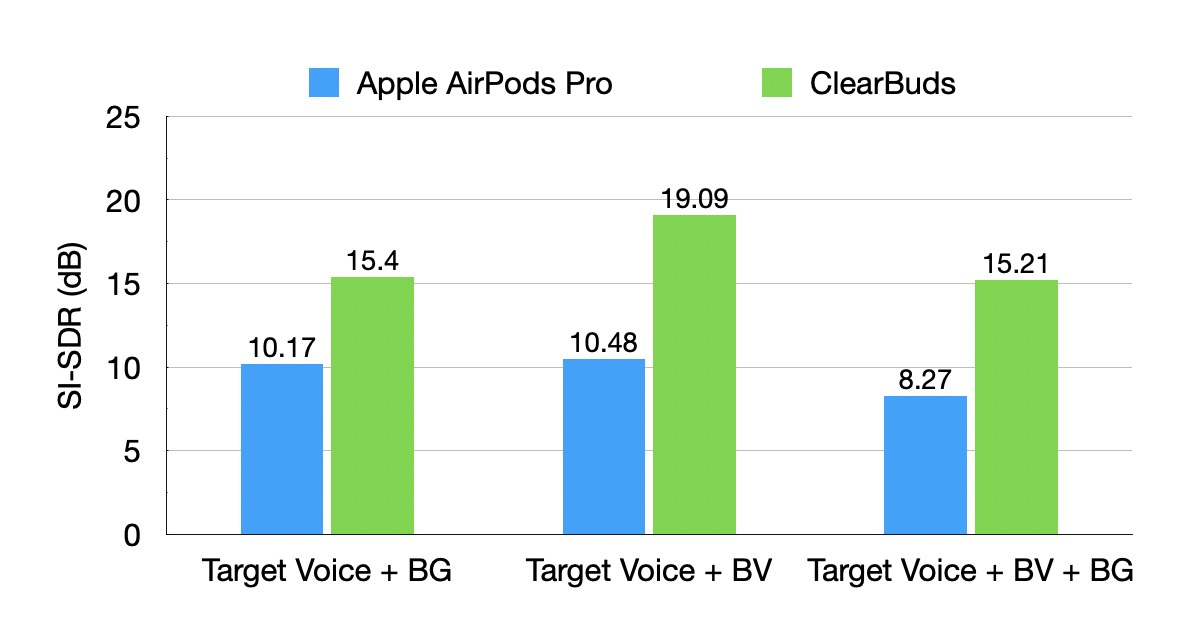
\includegraphics[width=0.65\linewidth]{CB_figures/AirPods_study_graph.png}
\vskip -0.2in
\caption{Comparison with AirPods Pro. Reporting the output SI-SDR (note: not SI-SDR increase). ClearBuds exceeds in three conditions: target voice plus background noise (BG), target voice plus background voice (BV), target voice plus background voice and noise.} % Data was collected with a mannequin head with artificial mouth and array of background monitor speakers.}
\vskip -0.15in
\label{fig:airpods}
\end{figure}

\section{Experiments and Results}
%We show several evaluations to demonstrate the strength of our method. First, we conduct a user study using completely in-the-wild recordings of a speaker in a noisy environment. Then we compare against AirPods using a repeatable audio setup that is run with both ClearBuds and with AirPods. To evaluate against baseline methods, we use quantitative metrics on the test set of the synthetic data and hardware data described in section \ref{sec:datasets}. Finally, we conduct several ablation studies with the synthetic dataset to show how various factors influence our speech enhancement quality. The system latency on a variety of mobile devices is also reported.

We first compare our end-to-end system performance against a commercial  wireless earbud system. We then present in-the-wild evaluation of our system. Next, we compare numerical results against various speech enhancement baselines. Finally, we present system-level evaluations. Our work is approved by the IRB.
%To compare our model's performance against that of other networks, we perform simulated experiments on synthetically rendered data as well as data collected from our ClearBuds hardware.
% To quantitatively compare our model's performance against that of other networks, we perform simulated experiments on rendered data.
% We then , we also collect data in a repeatable acoustic environment through our ClearBuds hardware.
% Next, we collect a variety of in-the-wild data and demonstrate the advantage of our hybrid network by running a \textcolor{red}{37 participant} user study and reporting mean opinion scores.
% We conduct several studies evaluating the effect reverberation, speaker angle, and ear distance.
% \textcolor{red}{Finally, we report measure and report system factors including synchronization, latency, and power consumption.}
\subsection{Comparison with  Beamforming Earbuds} \label{sec:endtoend}

 We  evaluate our end-to-end system against the Apple AirPods Pro headset connected to a  iPhone 12 Pro in a repeatable physical set up. In our evaluation, as is typical, there is  no overlap between training and test datasets. 


% %Loudness of target voice was about -22 dB as measured in recorded samples via ClearBud.

% During recording, qualitatively, it sounded like somebody talking loudly the room.
% %Loudness of ambient noise ranged between -38 and -22 dB.
% In input recorded samples, ambient noise SNR ranged between 0 dB and 16 dB with respect to target voice.
% Qualitatively, it sounded like a loud bar or a dense gathering.
%Loudness of side voice ranged -34 dB and -28 dB, 
% Side voice SNR ranged between 6 dB and 12 dB, qualitatively sounding like somebody speaking a meter or two away.

% \begin{table*}
%     %\vspace{-5mm}
% 	\centering
% 	\label{tab:real}
% 	\caption{Comparison against AirPods Pro. Numbers reported are the output SI-SDR (note: not SI-SDRi).}
% 	\small
% 	\begin{tabular}{c|ccc}
% 		\toprule
% 		& \multicolumn{3}{c}{Real Environment} \\  
% 		\midrule
% 		End-to-End System & {Target Voice + BG} & {Target Voice + BV} & {Target + BV + BG} \\
% 		\noalign{\vskip 1mm} 
% 		\hline
% 		\noalign{\vskip 1mm} 
% 		\textbf{ClearBuds}  & 15.40 & 19.09 & 15.21 \\
% 		Apple AirPods Pro & 10.17 & 10.48 & 8.27 \\
% 		\bottomrule
% 	\end{tabular}
% 	\label{fig:airpods}
% 	\vspace{-0.15in}
% \end{table*}




% Since Apple AirPods Pro do not zero pad dropped packets, misalignment can occur between test condition recording and reference recording over time, making it challenging to calculate SDR across all one hundred VCTK utterances at once. To overcome this, we align individual one second chunks and take the logarithmic mean across 250 chunks.


% \begin{figure*}
% \centering     
% \subfigure[]{\label{}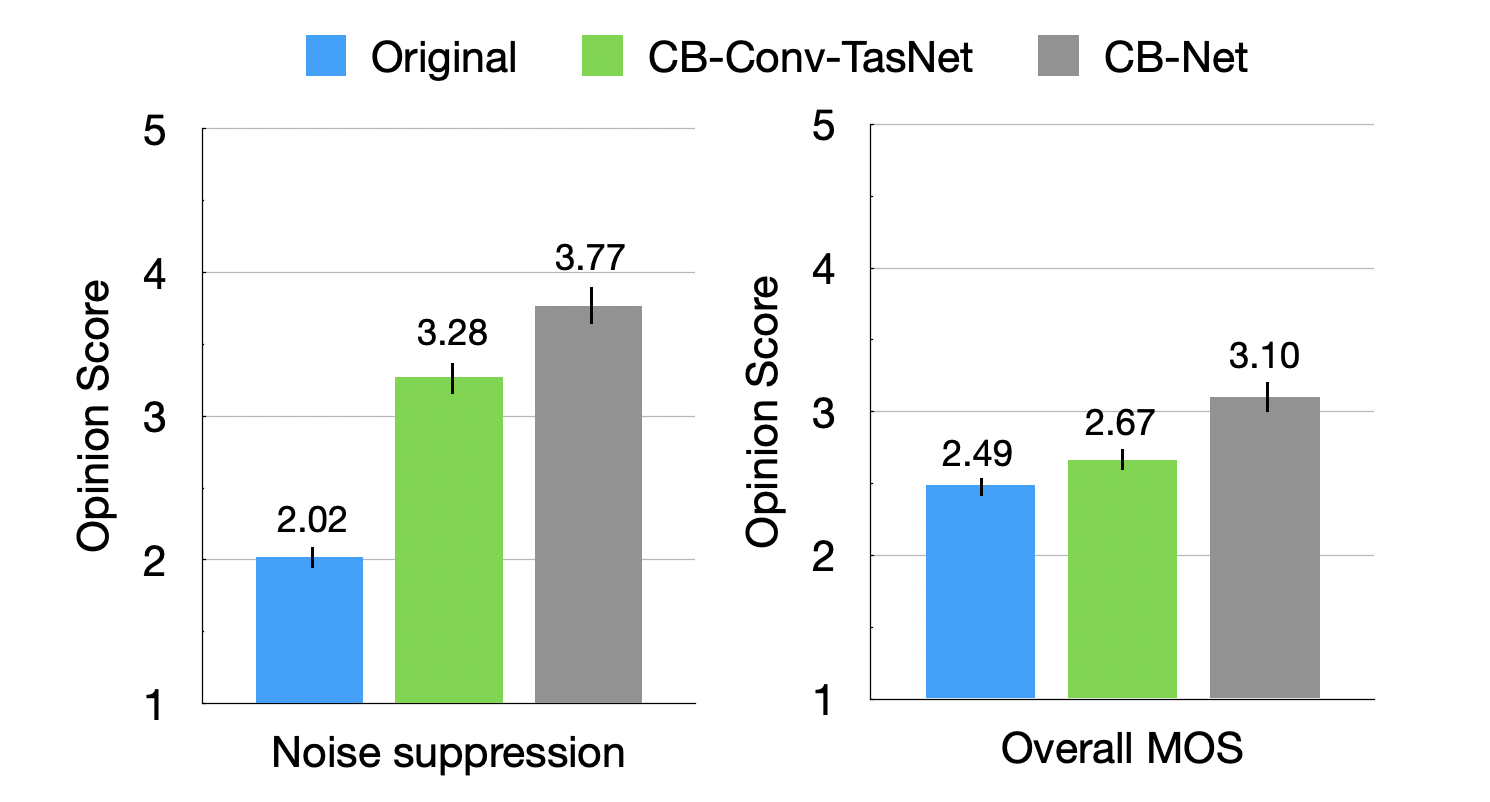
\includegraphics[width=0.5\textwidth]{CB_figures/MOS_study_results_v3.png}}\hfill
% \subfigure[]{\label{}\includegraphics[width=0.2\textwidth]{CB_figures/user-study-indoors-anon.jpg}}\hfill
% \subfigure[]{\label{}\includegraphics[width=0.2\textwidth]{CB_figures/user-study-outdoors-2-anon.JPG}}

% \subfigure[]{\label{}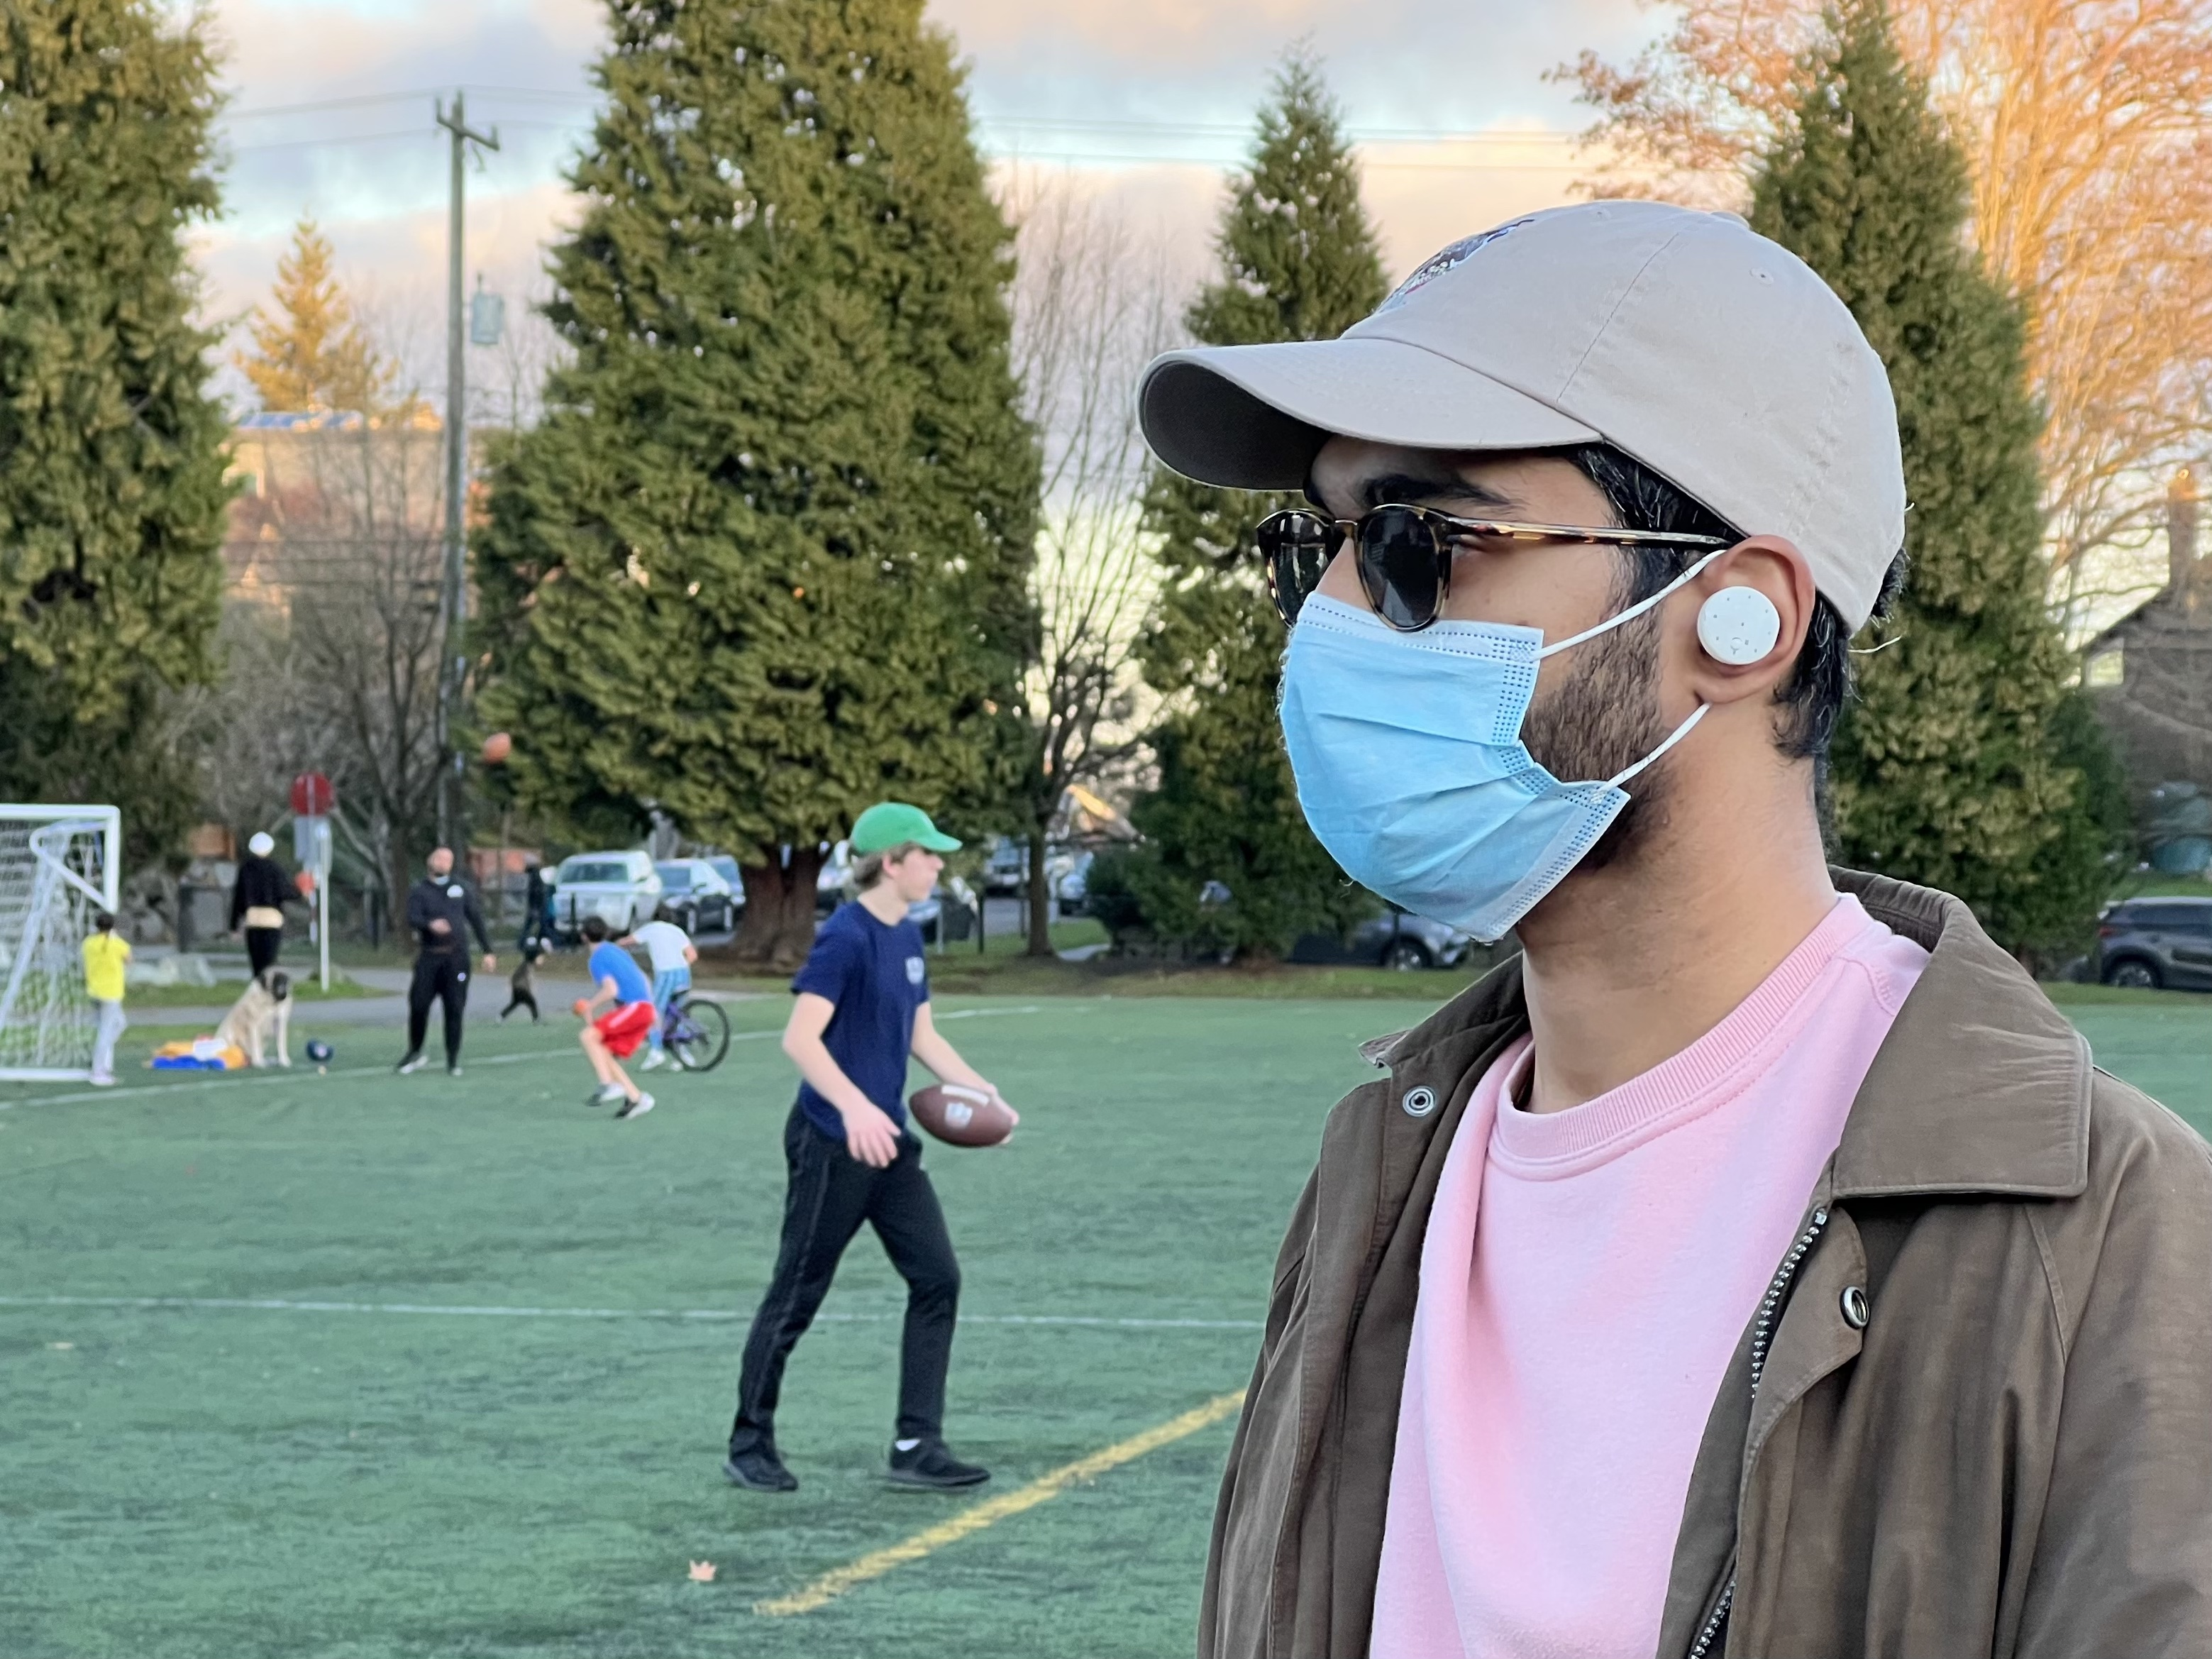
\includegraphics[width=0.2\textwidth]{CB_figures/user-study-outdoor-3.jpg}}\hfill
% \subfigure[]{\label{}\includegraphics[width=0.2\textwidth]{CB_figures/placeholder.jpg}}\hfill
% \vskip -0.15in
% \caption{(a) Mean opinion score study results. Noise suppression indicates perceived quality of background noise reduction (higher is less intrusive). MOS indicates overall perceived quality (higher is preferred). Error bars are 95\% CI. (b,c) Example scenarios (cafe, street) of where user study samples were collected. User study samples were collected across 10 users and 4 environments, all unseen in our training dataset.}
% \label{fig:mos-study-results}
% \vskip -0.2in
% \end{figure*}

\begin{figure*}
\centering  
%\begin{tabular}[c]{ccc}
%\multirow{2}{*}[14pt]{
%\subfigure[]{\label{}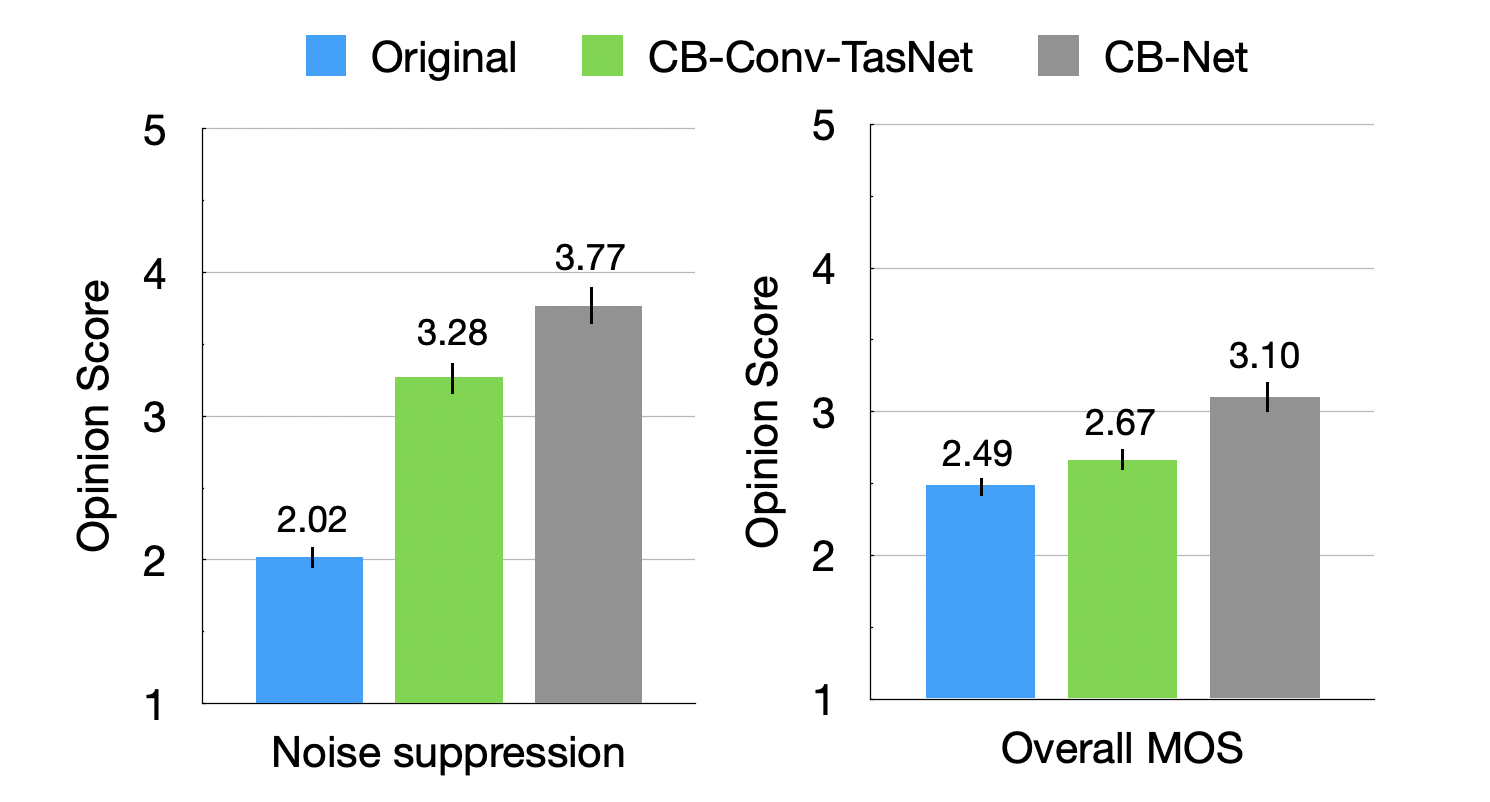
\includegraphics[width=0.5\textwidth]{CB_figures/MOS_study_results_v3.png}}}&
\subfigure[]{\label{}\includegraphics[width=0.24\textwidth]{CB_figures/user-study-indoors.jpg}} \hfill
\subfigure[]{\label{}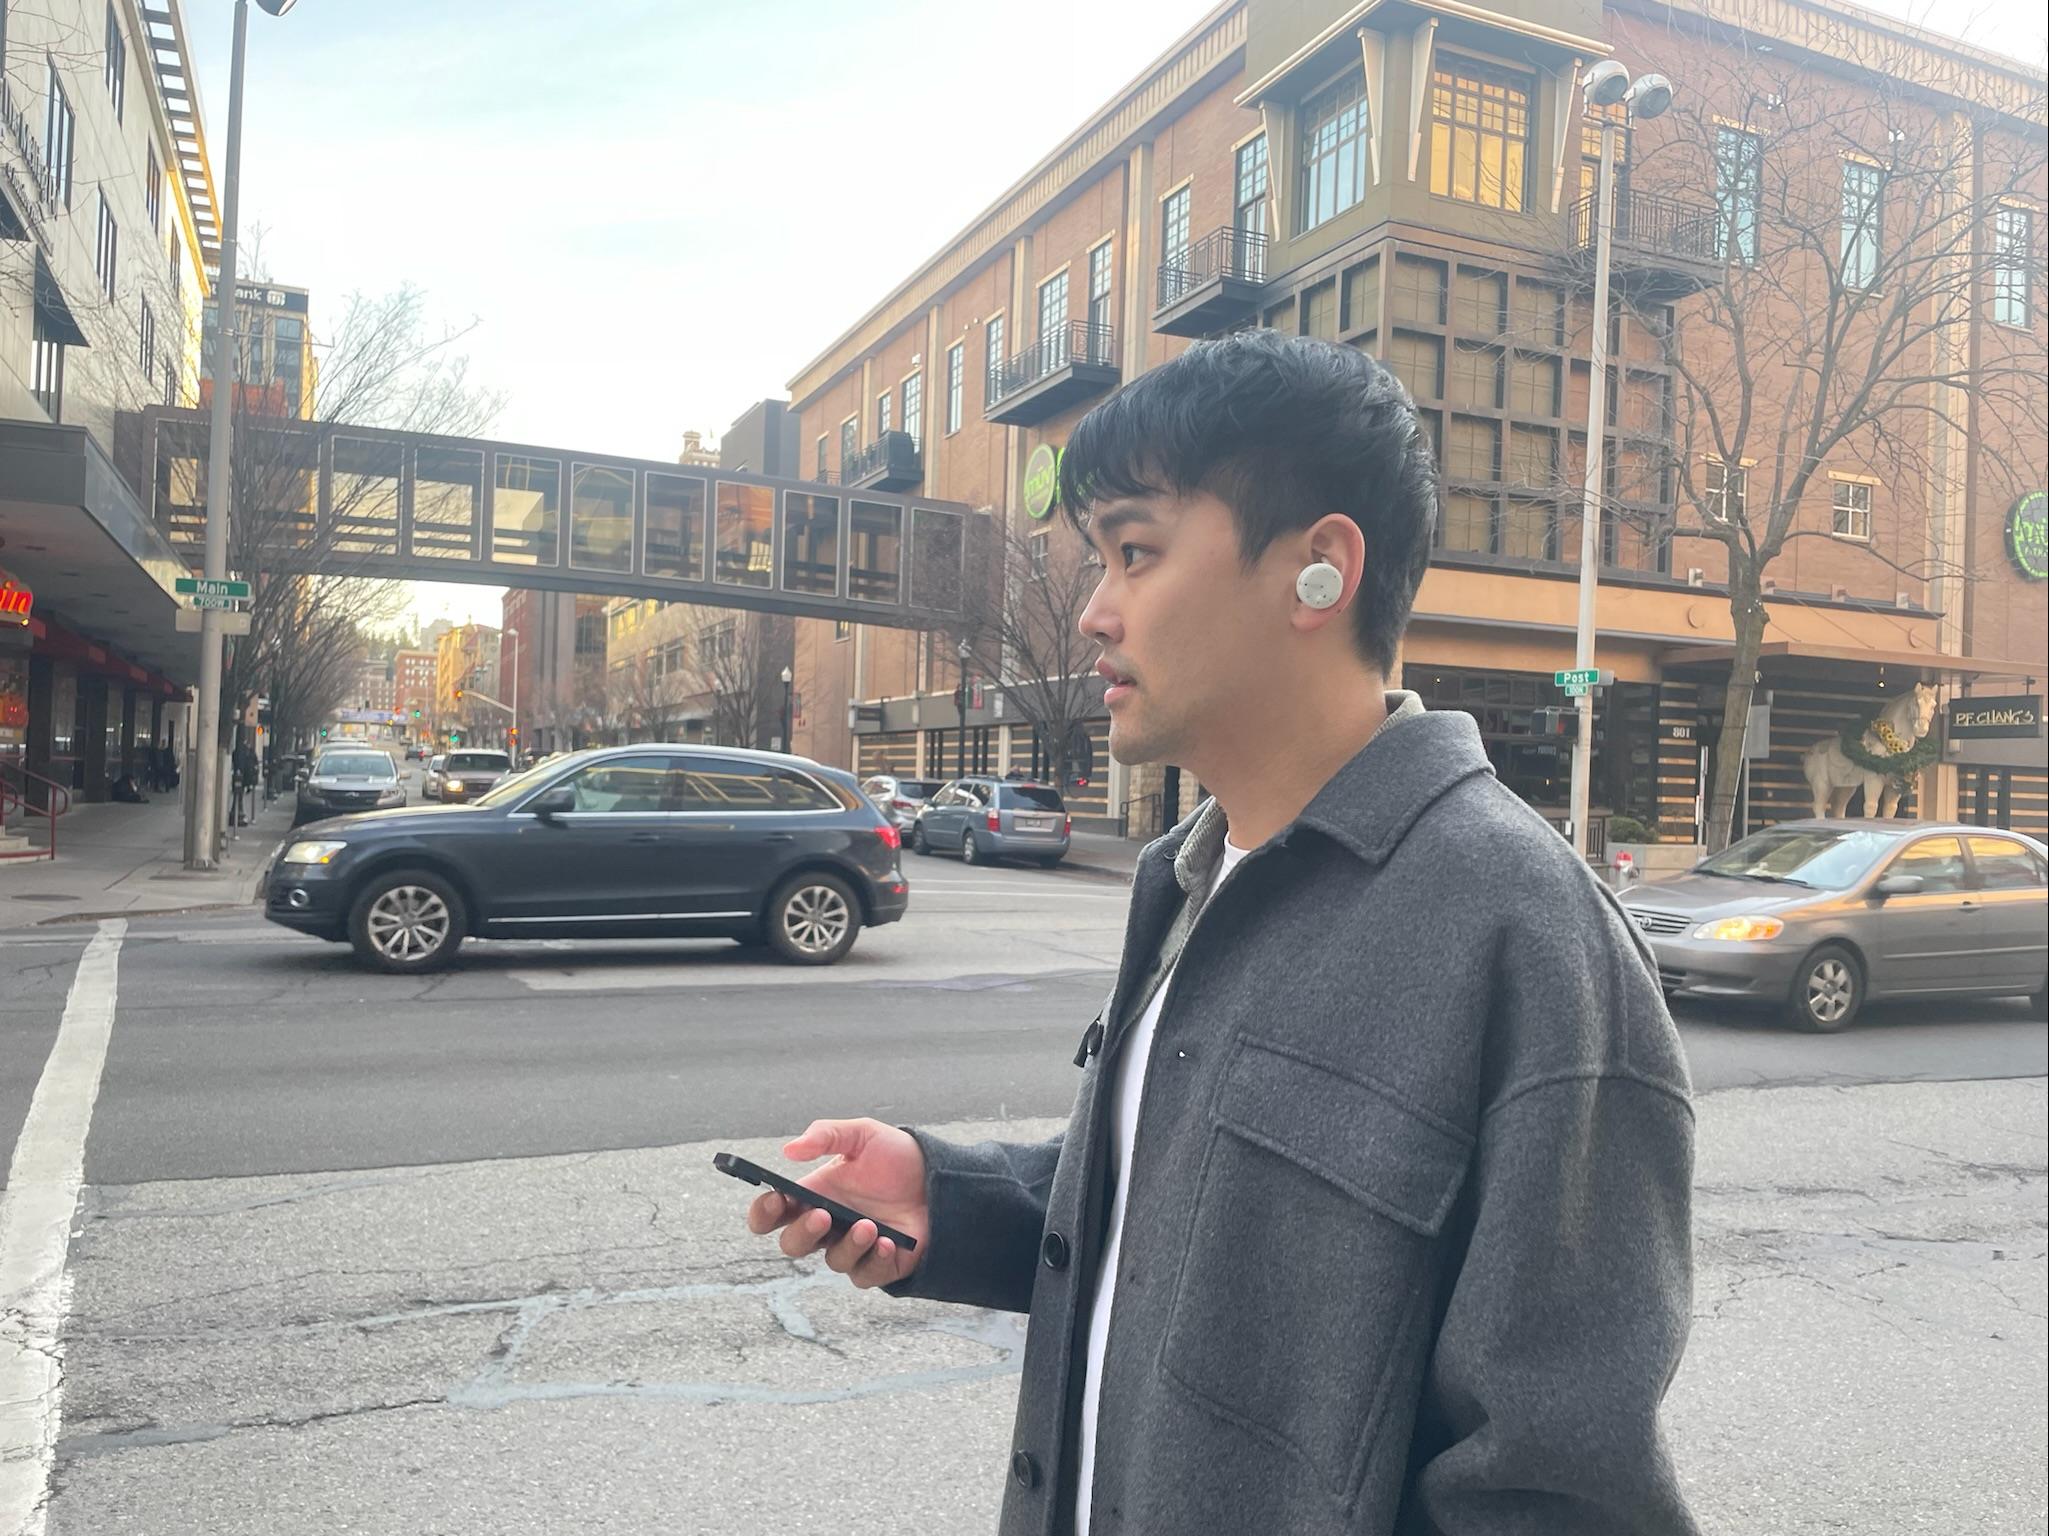
\includegraphics[width=0.24\textwidth]{CB_figures/user-study-outdoors-2.JPG}} \hfill
\subfigure[]{\label{}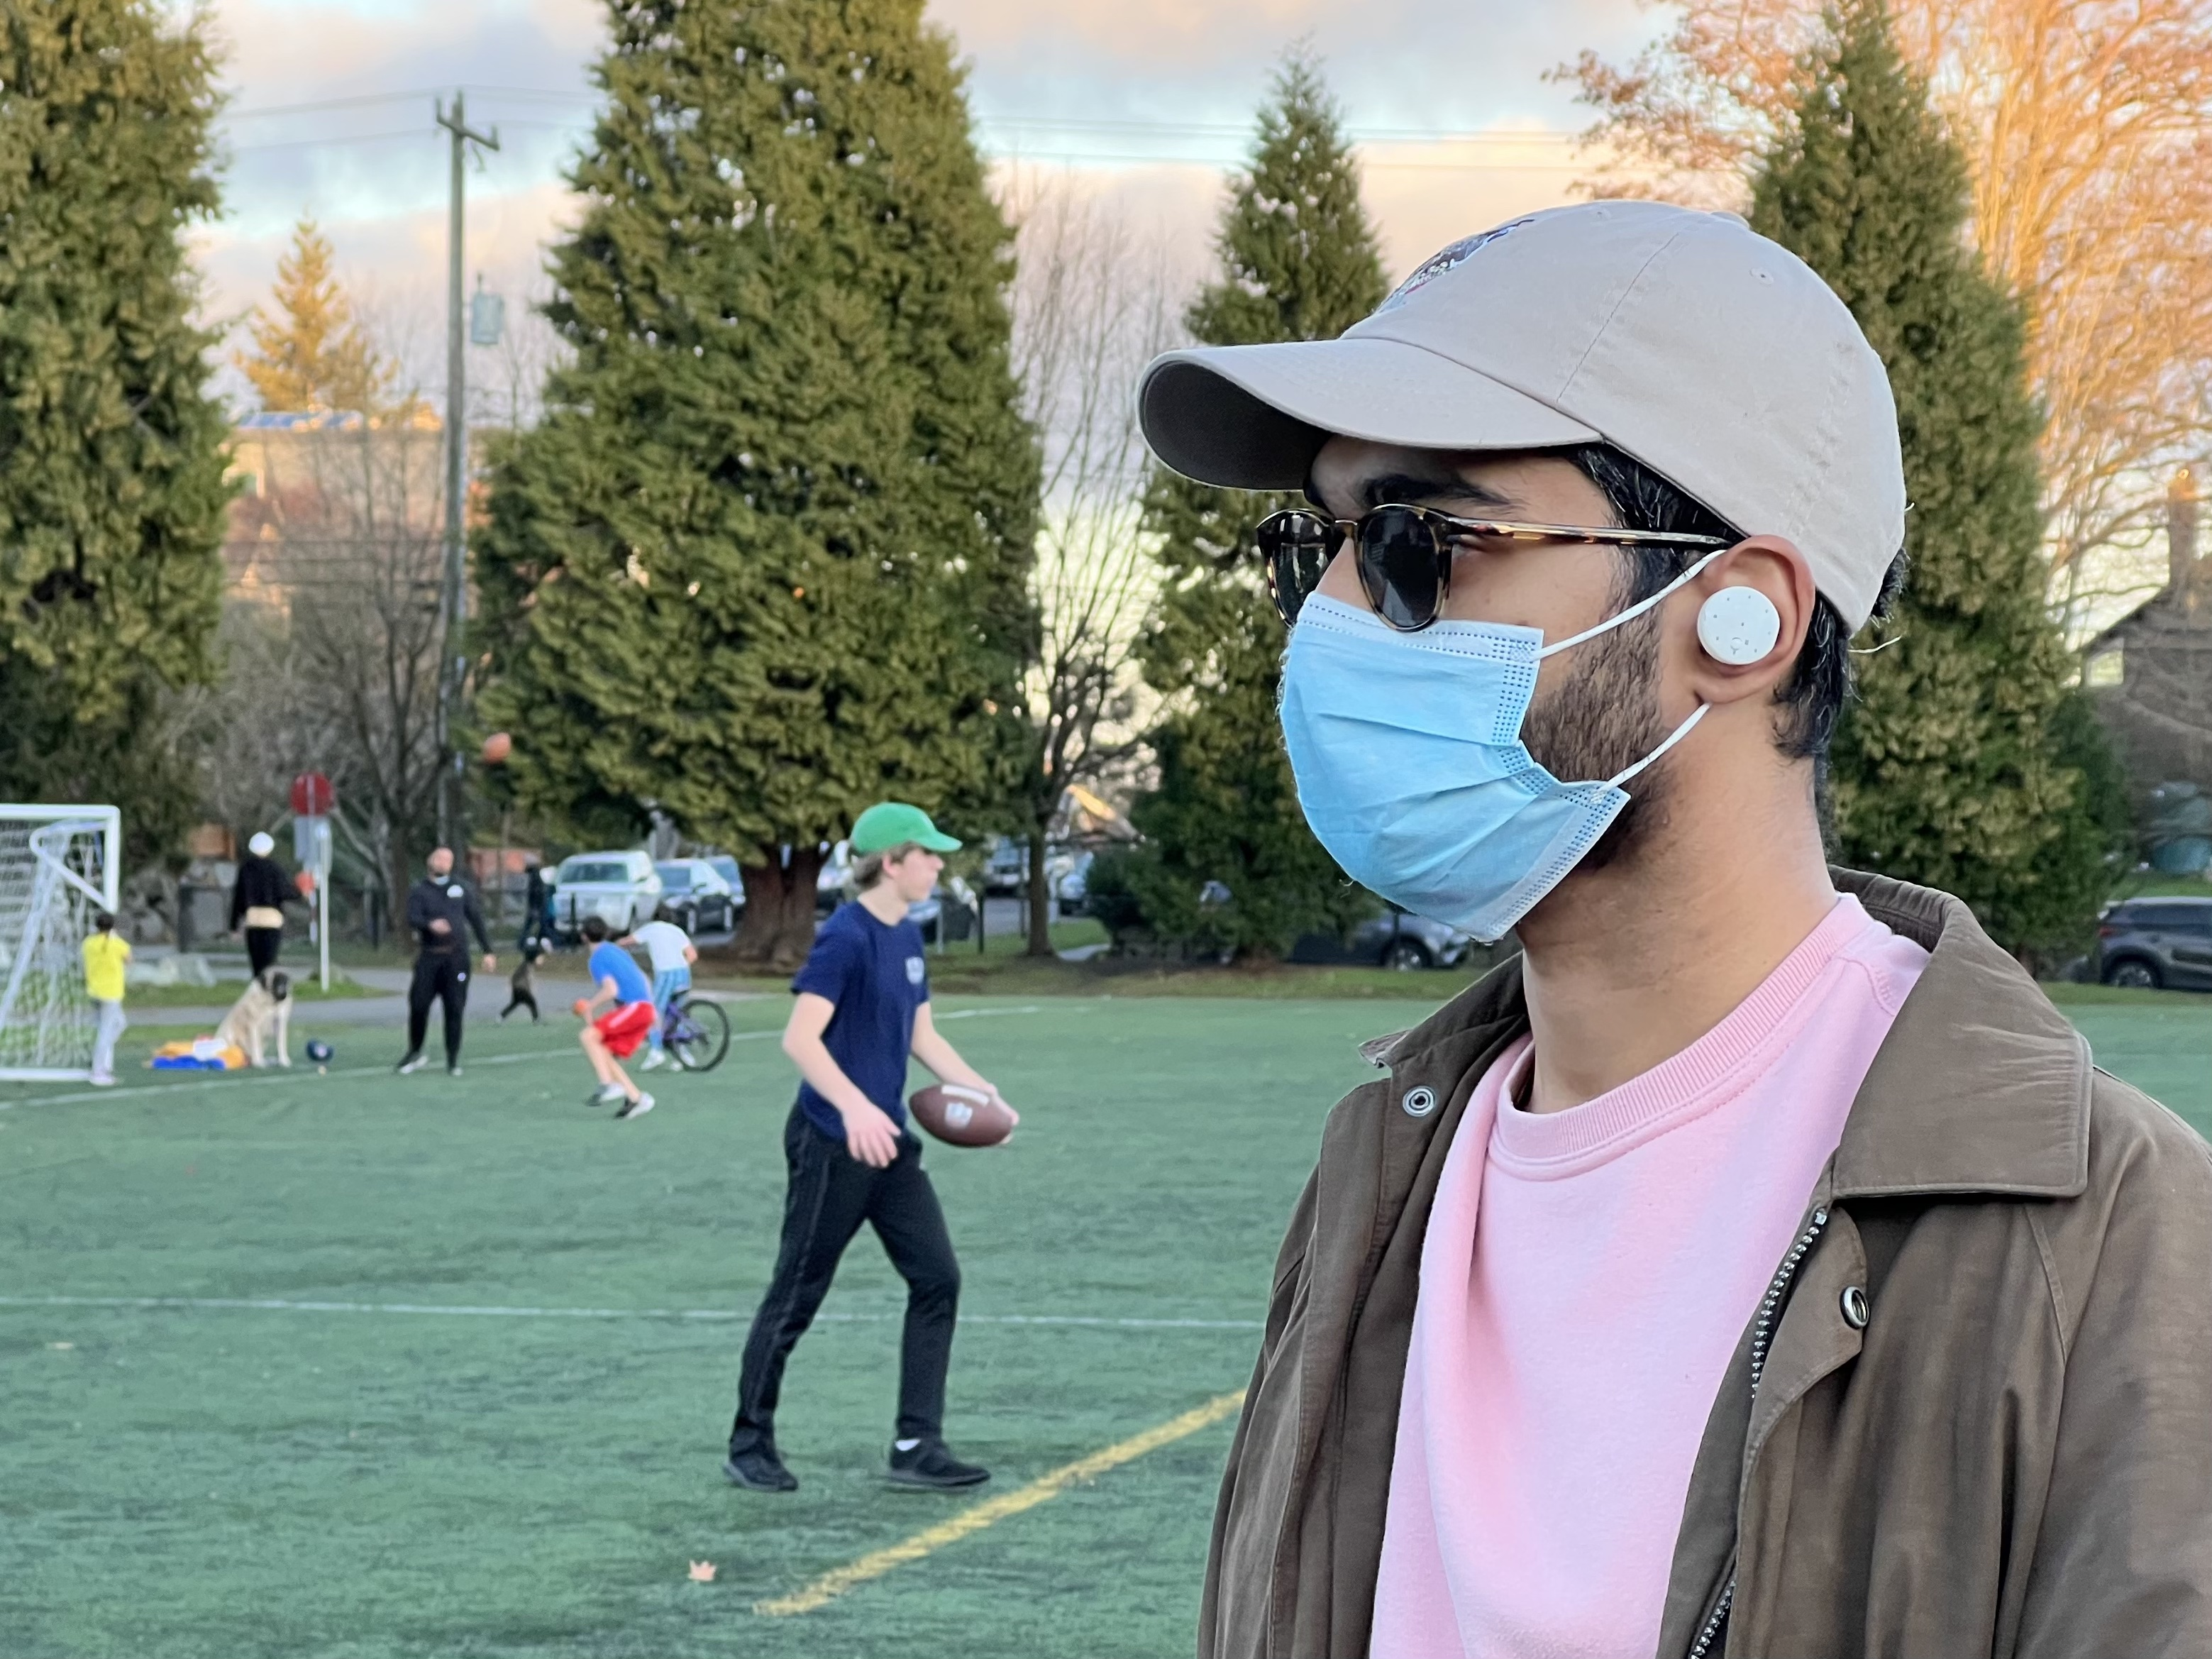
\includegraphics[width=0.24\textwidth]{CB_figures/user-study-outdoor-3.jpg}} \hfill
\subfigure[]{\label{}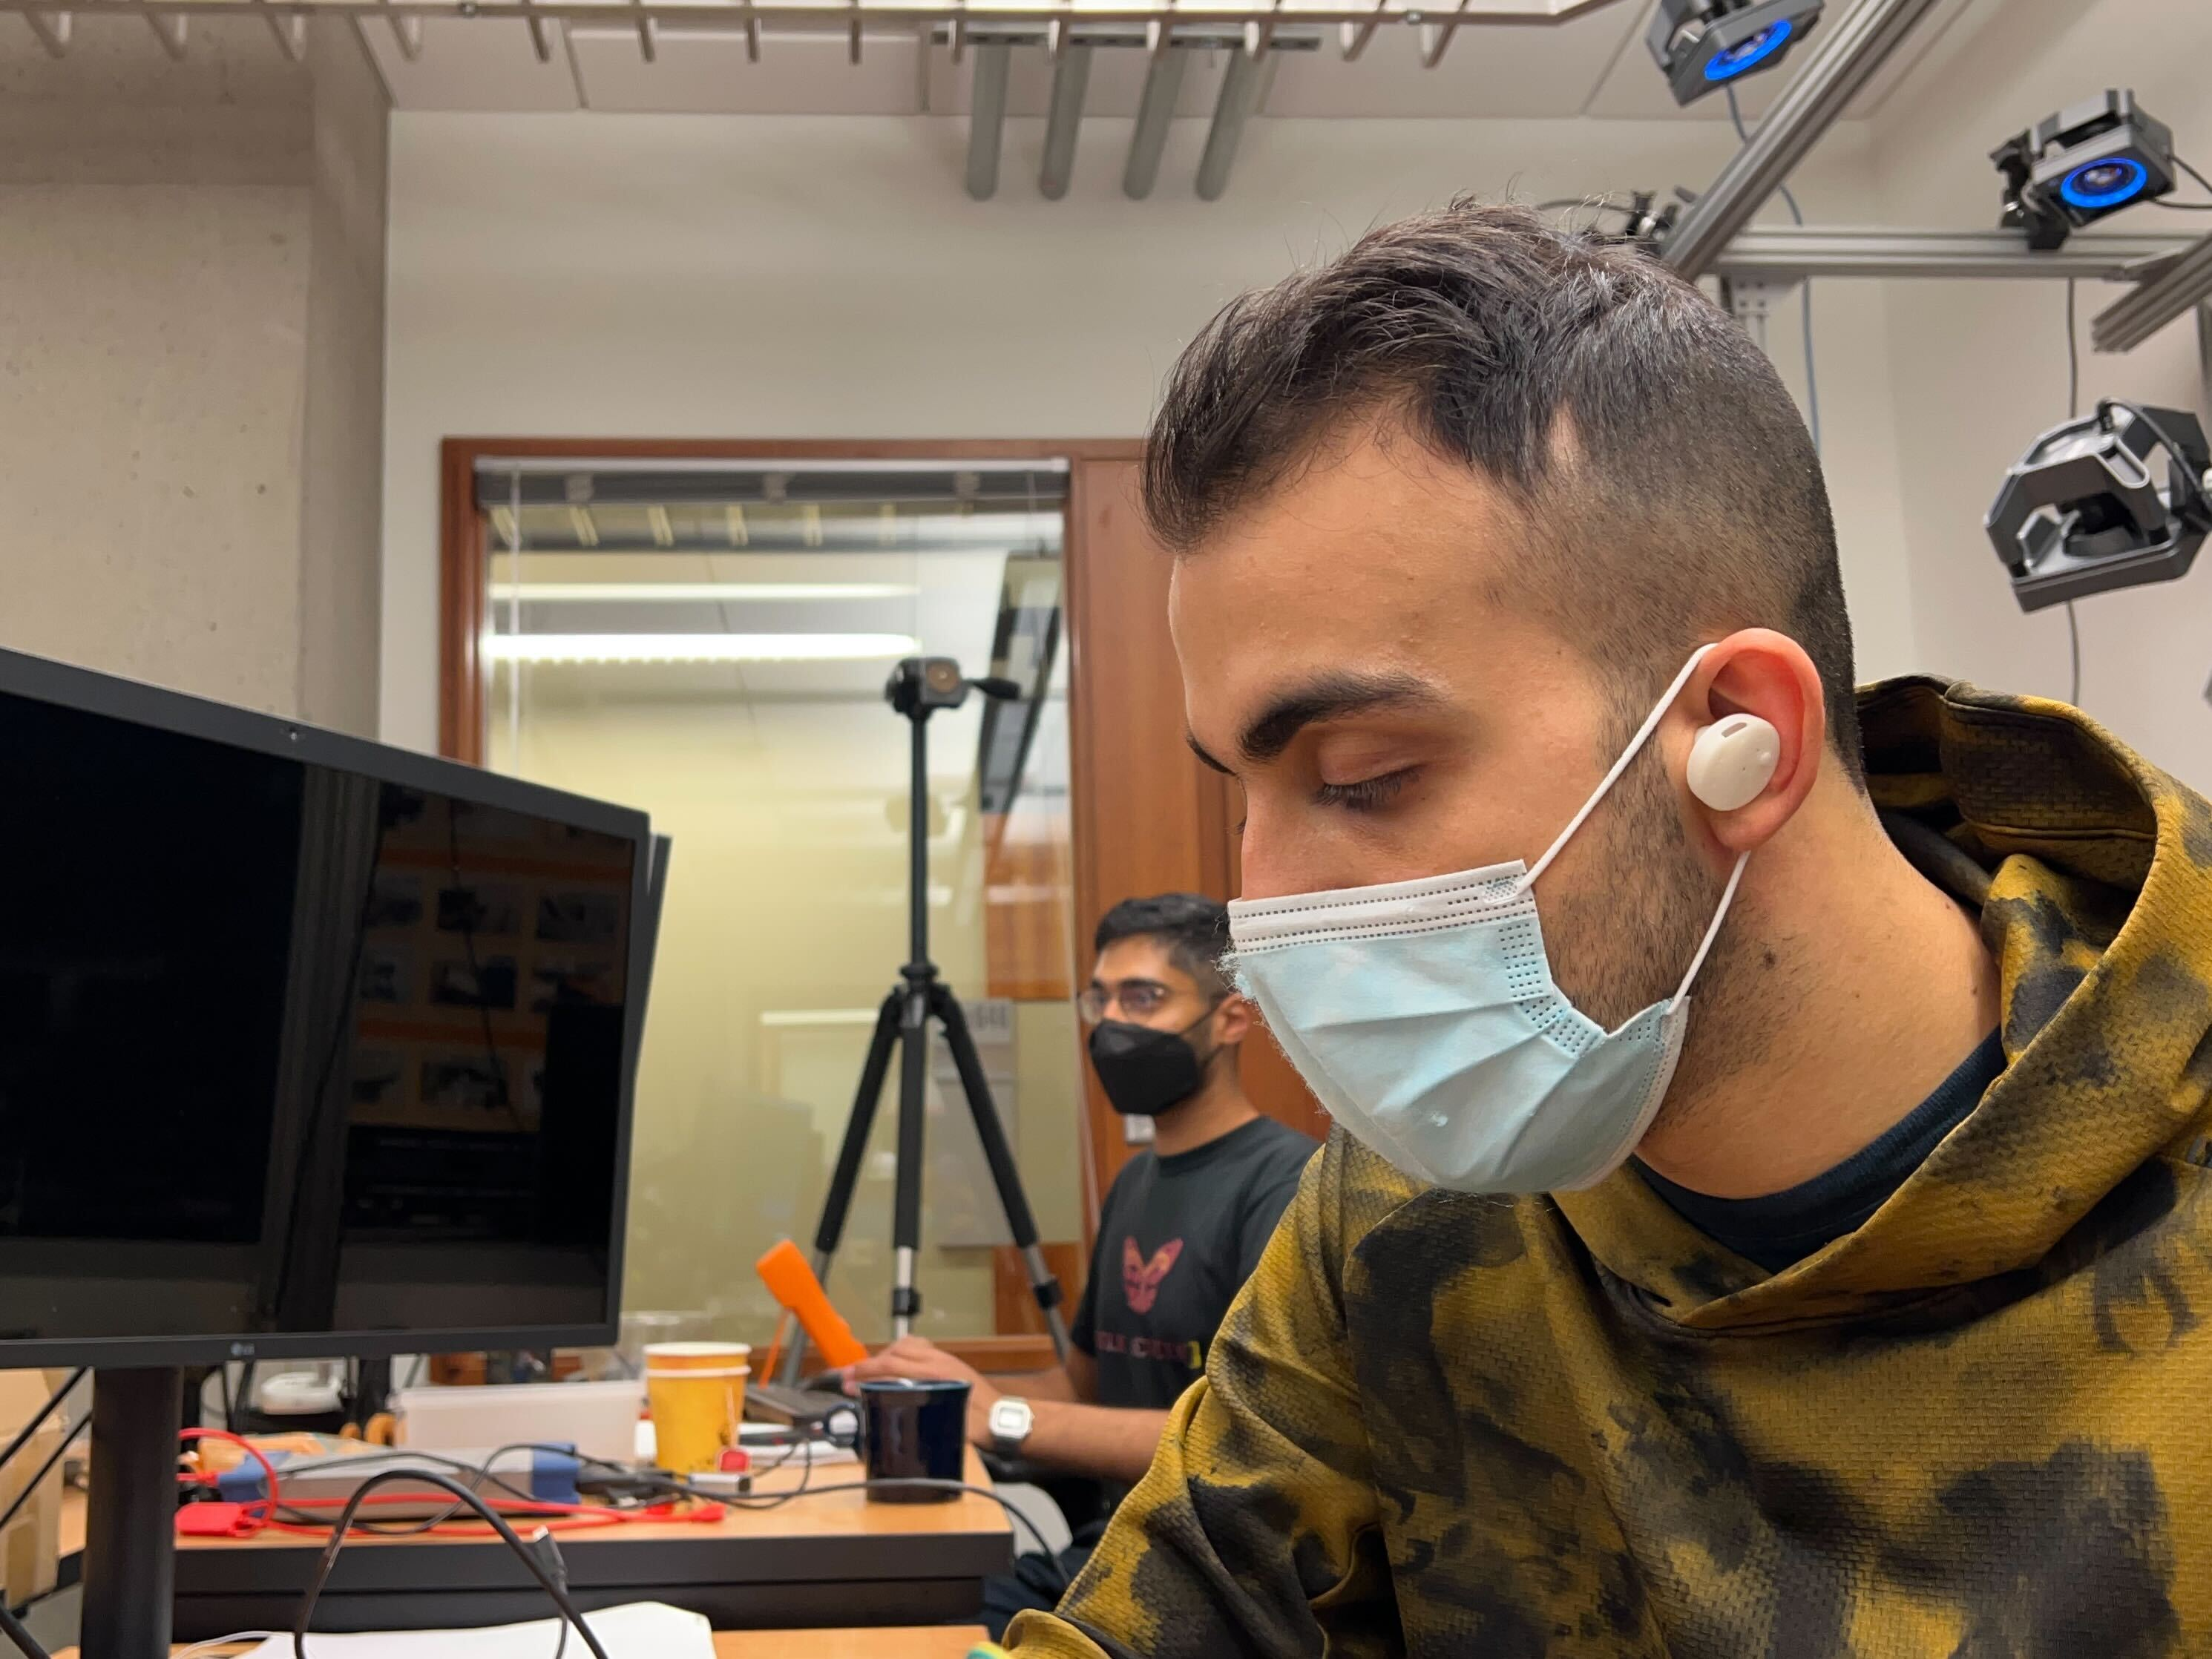
\includegraphics[width=0.24\textwidth]{CB_figures/user-study-indoor-env3.jpg}}\\
%\end{tabular}
\vskip -0.15in
\caption{{In-the-wild experiments in various  scenarios (crowded cafe, busy intersection, outdoor plaza, classroom)}  were conducted across 8 users and indoor and oudoor  environments, all unseen in our training dataset.}
\label{fig:picsenv}
\vskip -0.2in
\end{figure*}




{\bf Procedure.} We use the popular metric \textit{scale-invariant signal-to-distortion ratio} (SI-SDR)~\cite{sdr}. While SI-SDR provides a repeatable metric used in the acoustic community, it requires a clean, sample-aligned ground truth (target voice) as the basis for evaluation. Therefore, we create a repeatable soundscape for our test setup where a sample-aligned ground truth can be obtained.
A foam mannequin head with a speaker (Sony SBS-XB12) inserted into its artificial mouth uttered one hundred VCTK samples with identities and samples unseen in the training set. The mannequin wore ClearBuds and AirPods Pro in subsequent experiments, and the outputs of the two systems could be directly compared.
Ambient environmental sound (from WHAM! dataset) was played via four monitors (PreSonus Eris E3.5) positioned to fill 3 meter by 4 meter room, and background voice (also VCTK) was played from a monitor positioned 0.4 meters from head on the right. 
 %To create a repeatable soundscape for each test condition,
All speakers were driven through a common USB interface (PreSonus 1810c) ensuring the same time-alignment and loudness between the two  test conditions.
Since Apple AirPods Pro beamforming cannot be toggled on and off, we cannot calculate an SI-SDR increase (SI-SDRi), and therefore report output SI-SDR.
To establish the ground truth voice against which to calculate SI-SDR, we record clean target voice through each headset.
Ambient noise SNR ranged between 0dB and 16dB with respect to target voice. Qualitatively, this sounded like a second person speaking loudly in a noisy bar or cafe. Finally, background voice SNR ranged between 6dB and 12dB, qualitatively sounding like a person speaking from a meter or two away.


{\bf Results.}  We report output SI-SDR from the two systems in Fig.~\ref{fig:airpods}. To calculate output SI-SDR, we align individual one second chunks and take the logarithmic mean across 250 chunks. We find that ClearBuds achieves  higher output SI-SDR across all test conditions when  compared to the beamforming utilized by the Apple AirPods Pro. For a qualitative comparison of AirPods Pro versus ClearBuds performance with human speakers, see video: \textcolor{blue}{{{\url{https://clearbuds.cs.washington.edu/videos/airpods_comparison.mp4}}}}. %updated 2022-05-25

\subsection{In-the-Wild Evaluation}\label{sec:mos} 

We perform in-the-wild evaluation   in  indoor and outdoor scenarios as well as users not in the training data.
The procedure and results are described in the following sections.
% As described in section \ref{sec:nn}, in our hybrid network we apply an additional learned, low-cost spectrogram mask to clean unpleasant artifacts that surfaced when resource-constraining the Conv-TasNet architecture.
% As seen in Table \ref{table:results}, this change is not well characterized by SI-SDRi or PESQ metric as the SI-SDRi and PESQ of our CB-Conv-TasNet model did not differ from those of our hybridized, CB-Net architecture. So, we conducted a subjective listening test to comparing these conditions.


\begin{figure}
%\vskip -0.1in
\centering
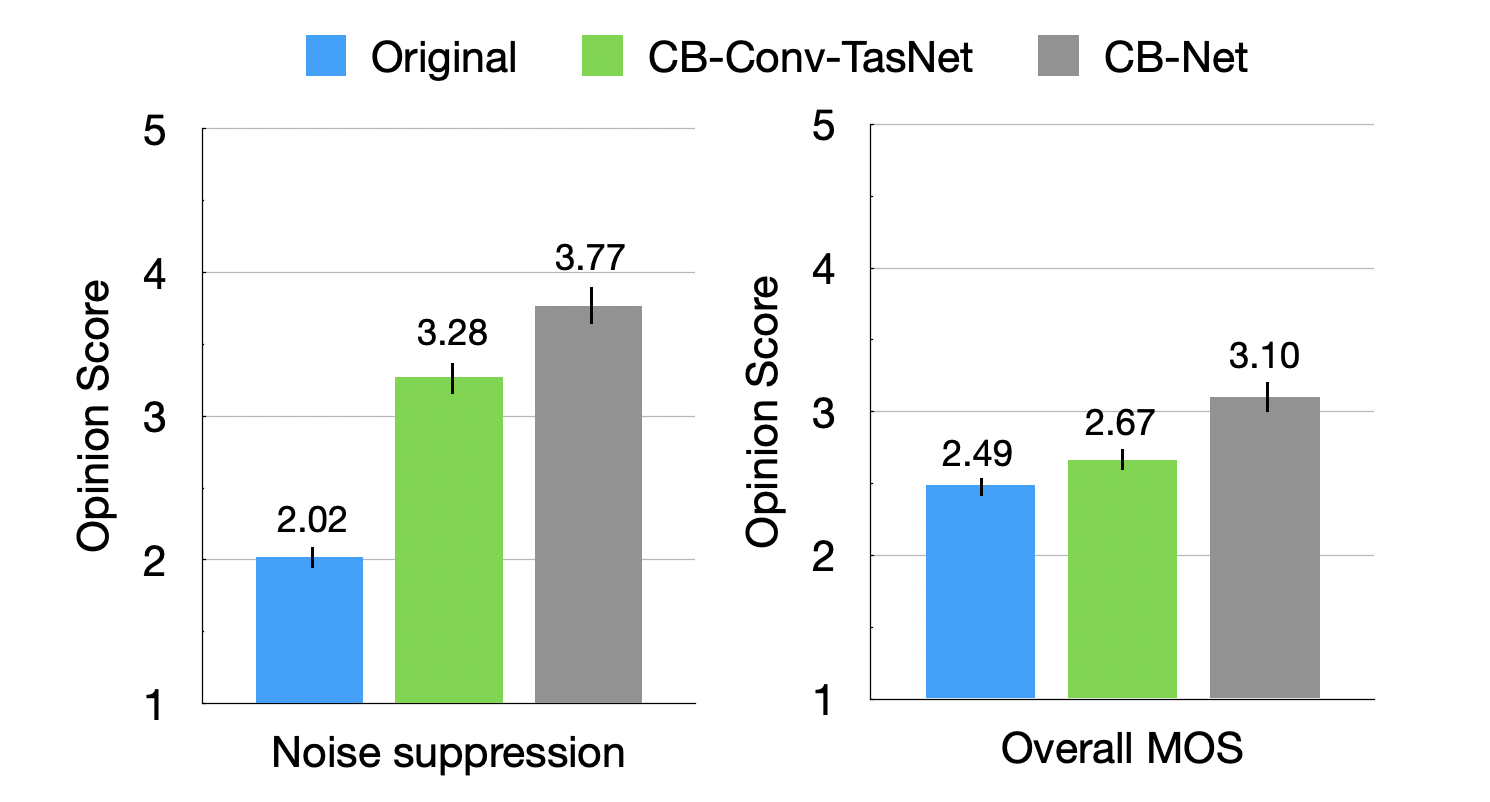
\includegraphics[width=0.65\linewidth]{CB_figures/MOS_study_results_v3.png}
\vskip -0.15in
\caption{In-the-wild study results. Noise suppression indicates perceived quality of background noise reduction (higher is less intrusive). Overall MOS indicates overall perceived quality. Error bars are 95\% CI.} % Data was collected with a mannequin head with artificial mouth and array of background monitor speakers.}
\vskip -0.2in
\label{fig:mos}
\end{figure}



{\bf In-the-wild experiments.} Eight individuals (four male, four female, mean age 25) with a variety of accents wore a pair of ClearBuds and read excerpts from Project Gutenberg~\cite{gutenberg}  while in four noisy environments: a coffee shop, a noisy intersection, an outdoor plaza, and a classroom (see Fig.~\ref{fig:picsenv}). The environments featured ringing phones, cross-talk from other people, ambient music, a crying baby, opening/closing doors, driving vehicles, and street noise, amongst other common sounds. These experiments  were uncontrolled in that the background voices and noise were naturally occurring sounds that are  typical to these real-world scenarios and were mobile.


{\bf Evaluation procedure.} In-the-wild evaluation precludes access to clean, sample-aligned truth to compute SI-SDR. Instead, the common (and expensive)  procedure is to perform a user study and compute the mean opinion score. Since this is a time-consuming process, prior works on binaural networks, e.g.,  \cite{luo2020endtoend, binaural_osu, jenrungrot2020cone}, avoid in-the-wild evaluation.  Since our goal is to design and evaluate an in-ear system in real scenarios, we recruit thirty-seven participants (11 female, 26 male, mean age 29)  for a user study. Each participant listened to between 6 and 11 in-the-wild audio samples (avg. 9.38 samples, each between 10--60 seconds). Each speech sample was processed and presented three ways: (1) the original input, (2) CB-Conv-TasNet, and (3) CB-Net, yielding a total of 37$\times$9.38$\times$3 $=$ 1,041 rating samples.
%Order of presentation was counter-balanced.

Participants were encouraged to use audio equipment they would typically use for a call. Fourteen used earbuds, thirteen used computer speakers, seven used headphones, and three used phone speakers. The study took about 25 minutes per participant. As is typical with noise suppression systems, participants were asked to give ratings in two categories: the intrusiveness of the noise and overall quality (mean opinion score - MOS):

\begin{small}
\begin{enumerate}
    \item \textbf{Noise suppression: }\textit{How INTRUSIVE/NOTICEABLE were the BACKGROUND sounds? 1 - Very intrusive, 2 - Somewhat intrusive, 3 - Noticeable, but not intrusive, 4 - Slightly noticeable, 5 - Not noticeable}
    \item \textbf{Overall MOS: }\textit{If this were a phone call with another person, How was your OVERALL experience? 1 - Bad, 2 - Poor, 3 - Fair, 4 - Good, 5 - Excellent}  
\end{enumerate}
\end{small}

\begin{figure}
\centering  
\subfigure[]{\label{}\includegraphics[width=0.23\textwidth]{CB_figures/street1.png}} %\hfill
\subfigure[]{\label{}\includegraphics[width=0.23\textwidth]{CB_figures/street2.png}}\\
%\end{tabular}
\vskip -0.15in
\caption{Mobility of speaker and noise sources in-the-wild. Red box highlights a moving truck on the road while ClearBuds user is walking.  Video: \linebreak \textcolor{blue}{\url{https://youtu.be/HYu0ybjcQPA?t=127}}}
\label{fig:mobility}
\vskip -0.2in
\end{figure}


{\bf Results.} Fig.~\ref{fig:mos} shows the noise intrusiveness and MOS values for the original microphone, CB-Conv-TasNet, and CB-Net.
As expected, applying CB-Conv-TasNet to the original audio helped suppress noise dramatically, increasing opinion score from 2.02 (slight better than \textit{2 - Somewhat intrusive}) to 3.28 (between \textit{3 - Noticeable, but not intrusive} and \textit{4 - Slightly noticeable}) (p<0.01).
The light-touch, spectrogram-masking clean up method featured in CB-Net increased noise suppression opinion score significantly (p<0.001) to  3.77, indicating the method did indeed further suppress perceptually annoying noise artifacts.
Importantly, this step also increased overall MOS. While users only slightly preferred (p<0.05) CB-Conv-TasNet (2.67) to the original input (2.49) due to artifacts introduced, they more significantly (p<0.001) preferred our  CB-Net (3.10), an increase of 0.61 opinion score points from the input.
For context, in the  flagship ICASSP 2021 Deep Suppression Noise Challenge \cite{icaasp_dns}, with state-of-the-art, real-time algorithms run on a quad-core desktop CPU, the winning submission increased MOS by 0.57~\cite{icaasp_dns_results} from input.



\begin{table*}
    \label{tab:sdr-results}
    %\vspace{-5mm}
	\centering
	\caption{ Benchmarking our neural network. We show results for a target voice speaking in three noise scenarios: (1) Background noise (BG), (2) Background voice (BV), and (3) Background noise and background voice (BG and BV).  CB-Conv-TasNet performs slightly better on  synthetic data, but as shown in Fig.~\ref{fig:mos}, does not generalize  as well to  in-the-wild  scenarios. This demonstrates the importance of evaluating  networks on real in-the-wild hardware data.}
	%\small
    \resizebox{1\textwidth}{!}{%
    	\begin{tabular}{c|ccc|ccc}
    		\toprule
    		& \multicolumn{3}{c}{SI-SDR increase (SI-SDRi)} & \multicolumn{3}{c}{Output PESQ} \\  
    		\noalign{\vskip 0.3mm}    
    % 		\toprule
    		\midrule
    		\noalign{\vskip 0.1mm}    
    		Method & \shortstack{Target with\\ BG} & \shortstack{Target with\\ BV} & \shortstack{Target with\\ BV + BG} & \shortstack{Target with\\ BG} & \shortstack{Target with\\ BV} & \shortstack{Target with\\ BV + BG} \\
    		\noalign{\vskip 1mm}    
    		\hline
    		\noalign{\vskip 1mm}    
    		\textbf{CB-Net} & 10.41 & 10.56 & 9.35 & 2.08 & 2.68 & 1.81 \\
    		CB-Conv-TasNet   & 11.19 & 11.01& 9.68 & 2.24 & 2.58 & 1.91 \\
    		CB-Conv-TasNet Single Mic & 6.15 & 0.13 & 2.34 & 1.82 & 1.84 & 1.53 \\
     		CB-UNet & 3.21 & 0.78 & 1.82 & 1.60 & 2.10 & 1.50 \\
     		{DTLN ~\cite{DTLN}} & 7.02 & 0.06 & 2.13 & 2.08 & 1.95 & 1.67 \\
    		Causal Demucs ~\cite{demucsreal} & 6.62 & -0.03 & 2.11 & 1.80 & 1.88 & 1.43 \\
    		Ideal Ratio Mask (IRM, oracle) & 11.41 & 11.53 & 12.04 & 2.53 & 3.00 & 2.44 \\
    		Ideal Binary Mask (IBM, oracle) & 9.97 & 11.05 & 10.85 & 2.30 & 2.90 & 2.21 \\
    %		Delay-and-Sum Beamforming & 1.97 & 0.89 & 1.32 & 1.67 & 2.02 & 1.56 \\
    		\bottomrule
    	\end{tabular}
    }
	\label{table:results}
\end{table*}


\begin{figure*}
\centering  
\vskip -0.15in %%% not \center
\subfigure[]{\label{fig:angle}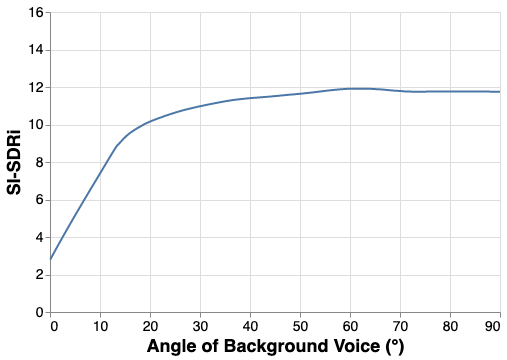
\includegraphics[width=0.3\textwidth]{CB_figures/angle-graph.png}}\hfill
\subfigure[]{\label{fig:reverb}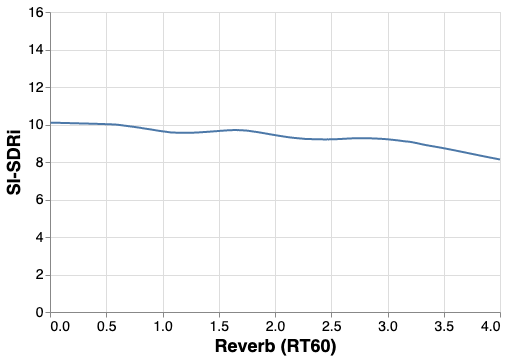
\includegraphics[width=0.3\textwidth]{CB_figures/reverb-graph.png}}\hfill
\subfigure[]{\label{fig:head-width}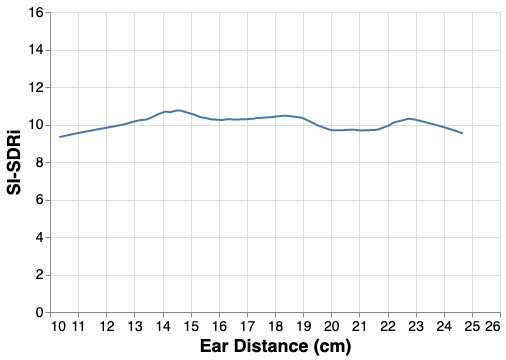
\includegraphics[width=0.3\textwidth]{CB_figures/ear-distance-graph.png}}
\vskip -0.15in
\caption{(a) Performance against angle of background voice in presence of significant multipath.  (b) Performance against amount of reverberation in an indoor room. RT60 (in seconds) measures how long sound takes to decay by 60 dB in a space with a diffuse soundfield. (c) Performance as distance between ears increases.}
\label{fig:ml-performance}
\vskip -0.2in
\end{figure*}


Note that in our in-the-wild experiments, the background noise and voices were not static. The speakers themselves can  also be  mobile (see Fig.~\ref{fig:mobility}). Our network was able to adaptively remove the background noise and achieve speech enhancement with  mobility. 


\subsection{Benchmarking our Neural Network}
The conventional evaluation in the machine learning and acoustic community is to evaluate models and techniques on synthetic data against baselines. For completeness, we compare our method against a variety of speech enhancement baselines using the synthetic dataset. For evaluation, an additional 1000 mixtures of 3 seconds each were generated such that there was no overlapping identities or samples between the train and test splits.


{\bf Evaluation Procedure.} For  comparisons to other baseline methods, we use the popular 
%the popular metrics \textit{scale-invariant signal-to-distortion ratio} (
SI-SDR  and {PESQ} metrics.
Unlike the AirPods experiment, where the original noisy mixture could not be recorded since AirPods beamforming cannot be toggled off, here we compute SI-SDR of the ground truth relative to both the input noisy mixture and then to the network output. When reporting the increase from the input SI-SDR to output SI-SDR, we use the  SI-SDR improvement (SI-SDRi).
%Unlike the AirPods experiment, where the noisy mixture could not be recorded, the SI-SDR of the ground truth here is computed relative to the noisy mixture and then to the network output. When reporting the increase from the input to output SI-SDR, we use the  SI-SDR improvement (SI-SDRi).

For a deep learning baseline in the waveform domain, we choose the causal Demucs model~\cite{demucsreal}. This is a single channel method which was recently shown to outperform many other deep learning baselines and runs real-time on a laptop CPU. We also compare with Dual-signal Transformation LSTM Network (DTLN) ~\cite{DTLN}. This method also runs on a laptop or mobile phone in real-time. To compare with spectrogram based methods, we use the oracle baselines, ideal ratio mask (IRM) and ideal binary mask (IBM) \cite{sigsep, wang2005ideal}, that use the ground truth voice to calculate the best possible result that can be obtained by masking a noisy spectrogram. 

As an ablation study, we report results with each individual component of the network,  \textit{CB-Conv-TasNet} and \textit{CB-UNet}. We also show results when the multi-channel part of our network, \textit{CB-Conv-TasNet}, only has access to one microphone, labeled as \textit{CB-Conv-TasNet Single Mic}. This explicitly shows the advantage of using two microphones.  There are only a few deep learning methods that tackle binaural speech separation for mobile processing, and the most relevant ones, such as \cite{binaural_osu} and \cite{han2020realtime}, do not have publicly available code to test against.



{\bf Results.} As shown in Table \ref{table:results}, our binaural method is comparable to the best possible results that can be obtained by a spectrogram masking method (IBM, IRM). We also show an improvement over waveform based deep learning methods that only use a single microphone input. In particular, the improvement is greatest when there are two speakers present (Target Voice + Background Voice). This is because single channel methods can only rely on voice characteristics, whereas our network also uses spatial cues to separate the speaker of interest. Although \textit{CB-Net} shows similar or worse performance to \textit{CB-Conv-TasNet}, subjective evaluation on in-the-wild hardware data shows that \textit{CB-Net} is far superior to human listeners (see~\ref{sec:mos}).

Examples of the synthetic dataset, outputs from all the methods and  qualitative comparisons against Krisp \cite{krisp}, a commercial noise suppression system, can be found linked from our project website: 
\textcolor{blue}{{{\url{https://clearbuds.cs.washington.edu}}}}.
%\textcolor{blue}{{{\url{https://bit.ly/3yJ6DwJ}}}}

%Further, to demonstrate our hybridized network's subjective background reduction and speech quality aspects, we run a  user study to compare the noise and speech performance amongst our mobile-deployed network architectures.



\subsubsection{Additional neural network  evaluations} We numerically evaluate various aspects of the design by changing the angle of background voice,  reverberance in the  environment, and microphone separation.

{\bf Angle of background voice.} The ability of our network to separate the target voice from a background voice is based on utilizing the time difference of arrival to the binaural microphones. Because we only have two microphones, this ability is limited when the background voice is in the front-back plane of the speaker. In this case, the background voice will arrive at each microphone simultaneously, and there will be no spatial cues to separate the two voices.  To illustrate this effect, we graph the separation performance as a function of the angle of the background voice in Fig.~\ref{fig:angle}. 


{\bf Multipath and reverberant environments.} While our in-the-wild experiments show the performance  in various indoor and outdoor environments, we benchmark our system  in different  reverberant conditions, including those more reverberant than seen during training. Synthetically generated mixtures are generated using the pyroomacoustics library  with the RT60 value randomly chosen between 0 and 4s. We generate 200 examples and plot the SI-SDRi compared to the RT60 in Fig.~\ref{fig:reverb}. Our method shows only a slight decrease in performance as the reverberation of the environment increases. Because the target speaker is physically close to the microphone array, our setup is generally less affected by reverberations than other kinds of source separation problems where the target speaker may be further away.

\begin{figure}
\centering     %%% not \center
\subfigure{\label{fig:sync-a}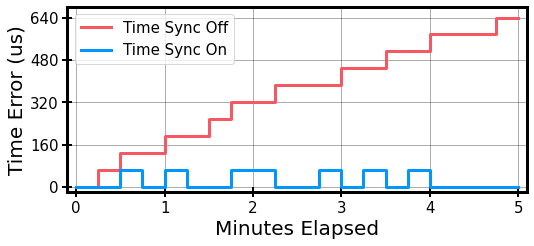
\includegraphics[width=0.36\textwidth]{CB_figures/sync.png}}%\vskip -0.12in
\subfigure{\label{fig:sync-b}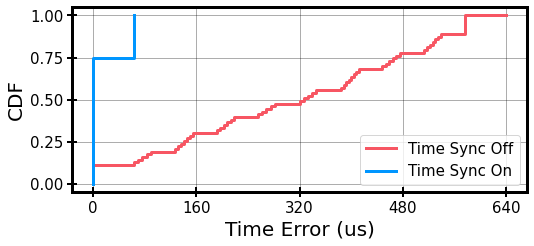
\includegraphics[width=0.36\textwidth]{CB_figures/time-sync-cdf.png}}
\vskip -0.15in
\caption{Time Synchronization Validation.  Without time synchronization (red), microphone samples drift apart and lose alignment at about 128$\mu$s/min.} %Also shows  CDF across three experiments of 5 minutes each. }
\label{fig:sync}
\vskip -0.2in
\end{figure}

{\bf Separation between microphones.} Our in-the-wild evaluation across 8 participants showed  generalization across facial features. Here, we  benchmark our method  to different head sizes where the distance between the microphones may be different. We generate 200 synthetic samples, where the distance between the microphones is randomly chosen between 10 and 25~cm. Because the target speaker is in the middle of the microphone array, the target signal will arrive at both mics simultaneously regardless of the microphone distance.  Fig.~\ref{fig:head-width} show little change in performance even with microphone distances greatly different than used during training.




\subsection{System   Evaluation}
%We evaluate various system parameters like synchronization, latency and power consumption. 
{\bf Synchronization.}  In order to evaluate this, we place both ClearBuds roughly equidistant from a speaker. A {click tone} is played every 15 seconds for 5 minutes, and recorded on both ClearBuds with time sync disabled and enabled. We calculate the sample error on each recorded click offline and convert it into time error with a sampling rate of 15.625kHz.
Fig.~\ref{fig:sync}(a) shows the synchronization  results across a five minute interval. With time sync enabled, the sample error never exceeds 1 sample at 15,625 kHz, or 64 $\mu$s. Fig.~\ref{fig:sync}(b) also shows the CDF of the timing error across  experiments of 5 minutes each conducted with other Bluetooth devices in the environment,  with and without time synchronization.  


{\bf Run-time and end-to-end latency.} Mouth-to-ear delay is defined as the time it takes from speech to exit the speaker's mouth and reach the listener's ear on the other end of the call. The International Telecommunication Union Telecommunication Standardization Sector (ITU-T) G.114 recommendation regarding mouth-to-ear delay indicates that most users are ``very satisfied'' as long as the latency does not exceed 200~ms \cite{g.114}. In our end-to-end system, we targeted a one-way latency of 100~ms prior to uplink, leaving up to 100~ms of network delay to move an IP packet from the source to the destination.

With a 180-sample PCM buffer being filled at 31.25 kHz, there is a 5.76~ms delay prior to the samples reaching BLE stack. Once these samples reach the radio hardware, there is a worst-case additional latency of 7.5~ms as defined by the minimum BLE connection interval supported by Bluetooth 5.0 \cite{bt5}. At the time of writing, the latest iOS supports a minimum BLE connection interval of 15~ms. After the samples reach the mobile phone, we wait for 67.2~ms to receive enough samples to run a forward pass of our network. Our network has a run-time of 21.4~ms on an iPhone 12 Pro (see Table~\ref{tab:latency}). The number of FLOPs is  computed over each packet of 350 samples. Together, we have a  latency of 109~ms, leaving 91 ms for  one-way network delay  (RTT=182ms).



{\bf Power analysis.} {CB-Net uses   an order of magnitude lower FLOPs per second compared to Conv-TasNet on the smartphone, significantly reducing the computational and corresponding power consumption. } We also  measure  the power consumption of the ClearBuds hardware. We measure current consumption by powering our system through its Micro-USB port with a DC power supply set to 3V, which goes through the same power path as our coin cell battery.
%We set our power supply voltage to 3V and set a maximum current output of 300mA, to reflect the internal 10 ohm resistance of a CR2032 battery.
While continuously wirelessly streaming microphone data, we measure average current consumed to be 5~mA. With the CR2032's nominal capacity of 210~mAh, this translates to approximately 42 hours of operation. Table \ref{tab:hardware-power-consumption} shows a breakdown by component of the system's power consumption. The accelerometer (BMA400) and flash (W25N01GVZEIG) are omitted as they are power gated during  streaming. 

%; mobile GPS usage reduces the battery-life by couple of hours

%\textcolor{red}{We also  ran our network on an  iPhone 12 Pro continuously after disabling all other applications except for Bluetooth and found that it took XXX hours to drain the battery on the phone starting at full charge.}


\begin{table}
	\centering
	\small
	\caption{ Neural network run time on smartphones }
	\begin{tabular}{ccccc}
		\toprule
		Device &  Conv-TasNet & CB-Conv-TasNet & \textbf{CB-Net} \\
		\noalign{\vskip 0.5mm} 
		\hline
		\noalign{\vskip 1mm} 
		iPhone 12 Pro & 155.5ms & 17.5ms & 21.4ms \\
		iPhone 11 & 165.4ms & 18.6ms & 22.7ms \\
		iPhone XS & 241.5ms & 27.2ms &  33.0ms \\
		\hline
		\noalign{\vskip 1mm} 
		FLOPs/packet & 1078M & 97M & 131M \\
% 		iPhone 12 Pro & 155.5ms & 17.5ms & 3.9ms & 21.4ms \\
% 		iPhone 11 & 165.4ms & 18.6ms & 4.1ms & 22.7ms \\
% 		iPhone XS & 241.5 & 27.2ms & 5.8ms &  33.0ms \\
		\bottomrule
	\end{tabular}
	\vskip -0.1in
	\label{tab:latency}
	%\vspace{-8mm}
	%\vskip -0.1in
\end{table}

\section{Limitations \& Future work}
% While ClearBuds presents state-of-the-art speaker separation in noisy environments, there are a few limitations to note for future work. 
The first limitation is that the user must be wearing both wireless earbuds to benefit from our binaural noise suppression network. Second, with only two microphones, there is an opportunity for background voices to remain in the uplink channel if the voice is within a few degrees of the target speaker's sagittal plane (see Fig.~\ref{fig:angle}). The underlying assumption of our network is that the mouth is in the middle of the user's ears, though as seen in Fig. \ref{fig:head-width} and our in-the-wild evaluation, some variance is permissible.

While we minimize the power consumption of the ClearBud hardware, we shift the processing and therefore power consumption to the more powerful mobile phone.  Performing network computation on the mobile phone over a cloud GPU is an enhancement in terms of user privacy and security so that sensitive voice data is not transmitted to the cloud.   While mobile chips are becoming more power efficient, an alternative design to explore is to run our neural network  on a plugged-in edge device (e.g., router),  minimizing computation while achieving similar latency.


{Future work could integrate two microphones in each earbud, so that each earbud could beamform toward the user's mouth prior to processing in the neural network. We also had to develop a custom wireless audio protocol to stream two microphones to a single phone. While this prevents this architecture from being deployed on today's commodity wireless earbuds, adoption may be imminent as Bluetooth 5.2 shows promise with the introduction of Multi-Stream Audio and Audio Broadcast \cite{le-audio-faqs}.}


{ Our network could also be deployed on other multi-microphone mobile or resource-constrained edge systems such as smart watches, augmented reality glasses, or smart speakers to allow for enhanced voice control or telephony in noisy environments. The hardware and firmware for Clearbuds could be leverage to produce wireless, synchronized microphone arrays for telephony, acoustic activity recognition or for swarm robot localization and control.} 

%But,  running the network on the GPU of the mobile phone comes at the cost of its  battery life.

\section{Conclusion}
Real-time speech enhancement has been an open research challenge for multiple decades. The recent proliferation of wireless earbuds and  neural network architectures provides an opportunity to build  systems that bridge neural networks and wireless earbuds to create new capabilities. Here, we present ClearBuds, the first deep learning based system to achieve real-time speech enhancement with binaural wireless earbuds. At its core is a new open-source wireless earbud design capable of operating as a synchronized binaural microphone array and a lightweight cascaded neural network. In-the-wild  experiments show that ClearBuds can achieve background noise suppression, background speech removal, and speaker separation using wireless earbuds. 

% Cite: https://www.twilio.com/blog/understanding-latency
% Cite: https://www.silabs.com/community/wireless/bluetooth/knowledge-base.entry.html/2015/08/06/audio_latency_withb-7BGG


% https://towardsdatascience.com/real-time-noise-suppression-using-deep-learning-38719819e051


 
 
 

% ========== Chapter 6

\chapter{[Proposed] OptoAcoustic Ring}

Starting with the smartphone, we increasingly interact with our computing devices on-the-go, a trend that shall continue as wearables including earbuds, smartwatches and smartglasses become more sophisticated and more integrated with our daily lives. Microgestures, or subtle motions of the fingertips, have been proposed as a compelling method of controlling these devices due to their low fatigue, high precision, social discreetness, and constant availability [cite].
%Thumb-to-index finger microgestures offer an ergonomic, subtle, and always-available method of providing gestural input.
Despite their subtlety, to operate the UIs associated with these devices, the fidelity of interaction afforded by microgestures should match the traditional display and touchscreen affordances on these devices including scrolling/panning in both dimensions, gestures like swipes, and buttons.

We propose OptoAcoustic Ring, a low-profile ring device that uses a miniature sparse, time-of-flight sensor or optical flow sensor and a skin-contact microphone to enable an interactive area on the tip of the index finger. These modalities to be inherently complementary with the optical sensor allowing for finger localization in $x$ and $y$ while the contact microphone can be processed to provide touchdown and swipe events.  

In OptoAcoustic Ring we aim to offer a set of unique features that surpass previous systems in terms of practicality. 
First, with OptoAcoustic Ring we aim to enable a variety of  thumb-to-index-finger microgestures. While previous ring-based systems can detect unistroke gestures such as swipes and circles, our look to make a system that  enables continuous 1D input in \textit{both} $x$ and $y$ dimensions as well as buttons.
Second, we hope to implement each of these microgesture interactions in a user-independent manner ensuring the device can be worn and used without calibration.
%In addition to the interaction being unobtrusive, the sensing methodology must  unobstrusive.
Third, we will design OptoAcoustic Ring to sit at the base of the finger similar to conventional jewellery. This positioning allows OptoAcoustic Ring's sensing stack to maintain a low profile unlike other optical-based systems where the optical sensor protrudes from the device to maintain line-of-sight  [cite] or capacitive methods which require obtrusive instrumentation of the fingertip [bleh].
Together these features can help to enable OptoAcoustic Ring to function in an in-context manner to control a pair of smartglasses.

To date, we have built a number of hardware prototypes using  miniature time-of-flight sensors. These sensors are a just several millimeters in each dimension, and provide 1-by-1 up to 8-by-8 pixels of depth data via direct ToF sensing.
After prototyping various configurations of one to four sensors with differing resolutions, we have arrived at a hardware configuration of a single ST VL53L7CX sitting at a 15-degree agree angle at the palm side of the base of the index finger. The angle is slight enough that the sensor remains relatively low-profile. We read a 90deg, 4-by-4 depth image of the shaft of the thumb from the perspective of the index finger at 30 Hz. Because of the depth image's low resolution, the sensor is inherently privacy preserving. However, this also makes it challenging to recover precisely what sensor is seeing, since there are no defining edges to distinguish. Therefore, we employ heuristics across the entire image to predict the \textit{x} and \textit{y} positions of the thumb tip on the first fingerpad of the index. First the depth data is inverted in direction and rescaled via a normal curve. This is so that we can easily threshold both far away pixels and noisy pixels together (after inversion and rescaling both tend to be close to zero) and also to provide additional resolution in the range of values associated with the finger depth. \textit{X} is calculated by a mean of the rescaled values. \textit{Y} is calculated by taking the weighted linear regression across all points. 

On the bio-acoustic sensing side, we aim to produce a classifier or heuristic that we can use to detect if the fingers are rubbing or tapping. We can use this to then accumulate gesture data from ToF during these events and trigger the appropriate interaction. The sound of the interaction itself may also contain information about the gesture. In this case we will need to design a multi-modal model structure to ingest both acoustic and ToF data streams.

We started prototyping with an IMU, however was unable to get good differentiation results using an ML classifier between typing, using the phone, rubbing hands, null, clapping, and our activity of interest -- rubbing fingertips. We think this is becuase we lack distinguishing information avialbe int he higher frequnecies, above 1 kHz. Instead, we are now using a much higher bandwidth contact microphone. We are still in the process of testing this sensor to understand whether it will give us better results but on the outset the spectrogram looks to carry much more information. We expect this classifier to be our main gating algorithm for triggering gestures even in active scenarios where the user is doing something else.

A limitation of our approach are the selected optical sensor is approximately 200--300 mW in continuous ranging mode, which is not very low power. However the sensor is designed to achieve  3.5m of ranging, so the transmit power is much greater than our required use case where the subject is 80 times closer. For the same target illuminance, the illumination power increases with the square of the distance. A customized sensor could allow for lower power without significant modification. Additionally the sensor could be turned on opportunistically when the bio-acoustic sensor sensor above a certain power threshold. Because we do not make strong use of the absolute position data returned the the ToF sensor, we will also consider optical flow sensors which can be used in extremely low power methods to detect whether the finger is approaching the sensor, moving away, moving up or down with respect to the sensor.

An additional limitation is that our prototype system thus far is a tethered  device. While we make effort to reduce the size of the sensing system itself to something that is low-profile, we are not attempting to miniaturize the signal processing electronics and will leave that to future work. 

We hope to target interactions that can be used to navigate a grid based 2D UI similar to what we see on a smartwatch or existing smartglasses. Our targeted gesture set would include  a set of no-calibration absolute buttons -- one at the fingertip, perhaps one in the middle of the fingerpad, and one near the first finger crease. We will also have a discrete unistroke gesture set containing CW and CCW cirlces and swipes up, down, left, right, and if possible the diagonals. Finally, we will target continuous x and y scrolling with automatic direction detection. This requires a very low latency determination of direction so that the scroll commences with the finger motion. Early prototyping suggests that full 2D "trackpad" is difficult to achieve without calibration across users due to differing hand geometry. At the edges of the motion, the finger is only partially in FoV of the ToF sensor and this looks very different person-to-person.

Finally, we will need conduct an evaluation that demonstrates the ring's ability to recover the targeted gesture set across people and scenarios. We will need to recruit users with a variety of hand shapes, colors and sizes. We will need to demonstrate the ring's ability to function and not trigger false gesture events even as the user is engaged in other activities, such as typing, using the phone, clapping, walking, and freeform movements.


% ========== Chapter 6

\chapter{Plan to Completion}

This final project is about 50\% completed. While the hardware is mostly complete and initial evaluations have been conducted, there is still work to be done:

% \subsubsection{May 2023:}
% Finalize \textit{x} and \textit{y} feature engineering. Finalize direction detection heuristic. IRB submitted.

% \subsubsection{June 2023:}
% Complete contact microphone processing and data pipeline. Collect microphone activity detection data and evaluate activity recognition performance. Consider progress and contribution to determine whether to submit in July 2023.

% \subsubsection{July 2023:}
% Considering progress, determine whether to run the user study and submit. If submitting, prepare example applications. If not submitted, re-assess ToF sensor selection and consider optical flow sensor. If switching sensors, finalize new hardware. Much of the same pipeline can be re-used.

% \subsubsection{August 2023:}
% Develop feature set with new sensor. Modify models as necessary. Re-train models.

% \subsubsection{September 2023:}
% Conduct user study. Submit.

% \subsubsection{October 2023:}
% Finalize dissertation.

% \subsubsection{November 2023:}
% Defend dissertation.


\vspace{2em}
\begin{tabular}{@{}lp{0.7\linewidth}@{}}
\textbf{May 2023} & Finalize \textit{x} and \textit{y} feature engineering. Finalize direction detection heuristic. IRB submitted. \\
\textbf{June 2023} & Complete contact microphone processing and data pipeline. Collect microphone activity detection data and evaluate activity recognition performance. Consider progress and contribution to determine whether to submit in July 2023. \\
\textbf{July 2023} & Considering progress, determine whether to run the user study and submit. If submitting, prepare example applications. If not submitted, re-assess ToF sensor selection and consider optical flow sensor. If switching sensors, finalize new hardware. Much of the same pipeline can be re-used. \\
\textbf{August 2023} & Develop feature set with new sensor. Modify models as necessary. Re-train models. \\
\textbf{September 2023} & Conduct user study. Submit. \\
\textbf{October 2023} & Finalize dissertation. \\
\textbf{November 2023} & Defend dissertation. \\
\end{tabular}



% ========== Chapter 7

\chapter{Conclusion}

Goals, design motivations

%\printendnotes
%
% ==========   Bibliography
%
\nocite{*}   % include everything in the uwthesis.bib file
\bibliographystyle{plain}
\bibliography{uwthesis}
%
% ==========   Appendices
%
% \appendix
% \raggedbottom\sloppy
 
% % ========== Appendix A
 
% \chapter{Where to find the files}
 


\end{document}
